%----------------------------------------------------------------
%	PACKAGES AND OTHER DOCUMENT CONFIGURATIONS
%----------------------------------------------------------------

\documentclass[12pt, english, singlespacing, parskip, headsepline]{MastersDoctoralThesis}

\usepackage[utf8]{inputenc}
\usepackage[T1]{fontenc}
\usepackage{palatino} %%% FONT

% BIBLIOGRAPHY
\usepackage[backend=bibtex,natbib=true]{biblatex}
\addbibresource{graphy.bib} % bibliography filename
\usepackage[autostyle=true]{csquotes}

\usepackage{fontspec}
\usepackage{xunicode}
\usepackage{hyperref}
\usepackage{xltxtra}
\setromanfont{FreeSerif}
\setsansfont{FreeSans}
\setmonofont{FreeMono}
\usepackage{mathtools}
\usepackage{pdfpages}
\usepackage{enumerate}
\usepackage{listings}
\usepackage{ulem}
\usepackage{float}
\usepackage{calrsfs}
\usepackage{amssymb}
\usepackage[utf8]{inputenc}
\usepackage{amsmath}
\usepackage{graphicx}
\usepackage{amssymb,amsmath}
\usepackage{hyperref}
\usepackage{paralist}
\usepackage{url}
\usepackage{xgreek}
\usepackage{epigraph}
\usepackage{color}
\usepackage{subcaption}
\usepackage{wrapfig}
\usepackage{enumitem}

%---------------------------------------------------------
%	MARGIN SETTINGS
%---------------------------------------------------------

\geometry{
	paper=a4paper, % Change to letterpaper for US letter
	inner=3cm, % Inner margin
	outer=3cm, % Outer margin (was 3.8)
	%bindingoffset=2cm, % Binding offset
	top=1.5cm, % Top margin
	bottom=1.5cm, % Bottom margin
	%showframe,% show how the type block is set on the page
}

% PARAGRAPHS (MINE == Maybe remove it)
%\setlength{\parskip}{\baselineskip}
\setlength{\parindent}{18pt}

%---------------------------------------------------------
%	THESIS INFORMATION
%---------------------------------------------------------

\thesistitle{Μελέτη και Αξιοποίηση Τεχνικών Ανάλυσης Μερικής Διαφυγής και Αντικατάστασης Βαθμωτών για Στατική Βελτιστοποίσηση στον Μεταγλωττιστή pypy}
\supervisor{Ιωάννης \textsc{Γαροφαλάκης}}
\examiner{}
\degree{Engineer's degree}
\author{Γεώργιος \textsc{Παπανικολάου}}
\subject{Computer Science \& Informatics}
\university{\href{http://www.upatras.gr/el}{Πανεπιστήμιο Πατρών}}
\department{\href{https://www.ceid.upatras.gr/}{Τμήμα Μηχανικών Η/Υ \& Πληροφορικής}}
\faculty{}

\hypersetup{pdftitle=\ttitle} % pdf's title
\hypersetup{pdfauthor=\authorname} % author

%---------------------------------------------------------
%	COLOR (CODE) SETTINGS
%---------------------------------------------------------

\definecolor{mygreen}{rgb}{0,0.6,0}
\definecolor{mygray}{rgb}{0.5,0.5,0.5}
\definecolor{mymauve}{rgb}{0.58,0,0.82}

\lstset{ %
  backgroundcolor=\color{white},
  basicstyle=\footnotesize,
  breakatwhitespace=false,
  breaklines=true,
  captionpos=b,
  commentstyle=\color{mygreen},
  deletekeywords={...},
  escapeinside={\%*}{*)},
  extendedchars=true,
  frame=single,
  keepspaces=true,
  columns=flexible, %
  keywordstyle=\color{red},
  language=Python,
  rulecolor=\color{black},
  numbers=left,
  showspaces=false,
  showstringspaces=false,
  showtabs=false,
  stringstyle=\color{mymauve},
  tabsize=2,
  title=\lstname
}

%---------------------------------------------------------
%	TITLE PAGE
%---------------------------------------------------------

\begin{document}
\frontmatter
\pagestyle{plain}

\begin{titlepage}
\begin{center}
\vspace{3 mm} %<<<<<<<<<
\begin{figure}[H]
\centering

\includegraphics[width=0.4\textwidth]{Upatras.jpg}
\end{figure}

\textsc{\Large Διπλωματική Εργασία}\\[0.5cm]

\HRule \\[0.4cm] % Horizontal line
{\LARGE \bfseries \ttitle}\\[0.4cm] 
\HRule \\[1.5cm] % Horizontal line
 
\begin{minipage}{0.4\textwidth}
\begin{flushleft} \normalsize
\emph{Author:}\\
\href{http://www.github.com/papanikge}{\authorname}
\end{flushleft}
\end{minipage}
\begin{minipage}{0.4\textwidth}
\begin{flushright} \normalsize
\emph{Supervisors:} \\
\href{http://athos.cti.gr/garofalakis/}{\supname}
\href{http://athos.cti.gr/nikolako/}{Αθανάσιος \textsc{Νικολακόπουλος}}
\end{flushright}
\end{minipage}\\[3cm]
 
{\large \today}\\[4cm]
 
\vfill
\end{center}
\end{titlepage}

\hyphenation{com-pil-er}
\hyphenation{com-pi-la-tion}


%-----------------------------------------------------------
%	QUOTATION PAGE
%-----------------------------------------------------------
\newpage\null\thispagestyle{empty}\newpage
\vspace*{0.2\textheight}

\noindent\textit{Nanos Gigantum Humeris Insidentes}\bigbreak

\hfill – Bernard of Chartres

%-----------------------------------------------------------
%	ABSTRACT PAGE
%-----------------------------------------------------------

\begin{abstract}
\addchaptertocentry{Περίληψη}

Αυτή η εργασία κατ'αρχάς συνοδεύει την απόπειρα βελτίωσης του υποσυστήματος
βελτιστοποίησης του μεταγλωττιστή PyPy μέσω της ανάλυσης διαφυγής. Αποσκοπεύει
επίπλέον στην πληροφόρηση του αναγνώστη σχετικά με την περίπλοκη "τέχνη" που
ακούει στο όνομα \textit{βελτιστοποίηση κώδικα} και τα προβλήματα που
αντιμετωπίζουν οι προγραμματιστές κατά την διαδικασία σχεδιασμού των
μεταγλωττιστών και κατά την υλοποίησή τους. Θα δώσουμε λεπτομέρειες σχετικά με
γενικά προβλήματα για ανάπτυξη δυναμικών γλωσσών καθώς επίσης και συγκεκριμένα
για την Python και το σύστημα PyPy. Έπειτα θα αναλύσουμε τις θεωρητικές
λεπτομέρειες για σχεδιασμό μεταγλωττιστών και συγκεκριμένα για στατική ανάλυση
κώδικα βάσει γραφημάτων, μερική ανάλυση διαφυγής και αντικατάσταση βαθμωτών.
Κύριος σκοπός της εργασίας αυτής είναι η σχεδίαση ένος backend module για το
σύστημα PyPy που θα υλοποιεί την μερική ανάλυση διαφυγής. Η δουλεία είναι
βασισμένη σε ένα προηγούμενο paper που αποτελεί υλοποίηση και μελέτη για την
γλώσσα Java. Το module θα αποτελέσει παράδειγμα για την θεωρία που θα αναλύσουμε
αλλά θα προσπαθίσουμε επίσης να το είσαγουμε στο όλο codebase του project έτσι
ώστε να συμβάλουμε στην βελτίωση του μεταγλωττιστή. Τέλος η εργασία θα
περιλαμβάνει φυσικά μετρήσεις και benchmarks.


\end{abstract}

%---------------------------------------------------------------
% SECOND ENGLISH ABSTRACT (VERBATIM AND INLINED !!!)
\newpage\null\thispagestyle{empty}\newpage
\checktoopen
\tttypeout{\abstractname}
\null\vfil
\thispagestyle{plain}
\addchaptertocentry{English Abstract}
\begin{center}
{\normalsize \MakeUppercase{\href{http://www.upatras.gr/en}{University of Patras}} \par}
\bigskip
{\huge\textit{Abstract} \par}
\bigskip
{\normalsize \href{https://www.ceid.upatras.gr/en/}{Computer Engineer \& informatics Department} \par}
\bigskip
{\normalsize Engineer's Degree\par}
\bigskip
{\normalsize\bfseries Study and Implementation of Partial Escape Analysis and Scalar
Replacement Methods for Static Optimization in the PyPy Compiler Framework \par}
\medskip
{\normalsize Georgios Papanikolaou \par}
\bigskip
\end{center}

This document, first and foremost, is the companion of an attempt to improve the
escape analysis optimization of the PyPy interpreter. However, it also aims to
shine light at the peculiar craft of compiler optimization and will try to
inform the reader of the nuisances and problems that the engineers face
throughout the designing process. We will elaborate on general problems based on
dynamic language design, as well as problems that we experienced specifically
with Python and with the PyPy framework. Furthermore we will expand on the
details of compiler optimization with intricate details on the static analysis
of graphs, partial escape analysis and scalar replacement. The main goal is the
design and the implementation of a backend optimization module for PyPy that
performs partial escape analysis. It is based on a previous treatise of the same
subject – an implementation for Java. It will serve as an example of the said
theory, and we will also try to fully integrate it into the whole PyPy project,
in order to improve the overall speed of the interpreter. Last, but not least,
we will accompany our implementation with benchmark and measurements.

%-----------------------------------------------------------
%	ACKNOWLEDGEMENTS
%-----------------------------------------------------------

\newpage\null\thispagestyle{empty}\newpage
\thispagestyle{plain}
\begin{center}{\huge\textit{Acknowledgements – Ευχαριστίες}\par}\end{center}
\vspace{3cm}

I'd like to thank Carl Friedrich Bolz for his valuable and eye-opening help with
the theory that this text entails and his aid with the debugging, my official
supervisors for their help, acceptance and tolerance of my quirks and last but not
least my parents for their financial and moral help. Thank you guys.

%-----------------------------------------------------------

%% TOC:
\tableofcontents

%%%%%%%%%%%%%%%%%%%%%%%%%%%%%%%%%%%%%%%%%%%%%%%%%%%%%%%%%%%%
%	THESIS CONTENT - CHAPTERS
%%%%%%%%%%%%%%%%%%%%%%%%%%%%%%%%%%%%%%%%%%%%%%%%%%%%%%%%%%%%

\mainmatter % Begin numeric arithmetic

\pagestyle{thesis}

%------------------------------------------------------------------------------

\chapter{Εισαγωγή}
\label{chapter1} % \ref{}

\section{Γενικά}

Σε αυτό το κεφάλαιο αποσκοπούμε να ενημερώσουμε τον αναγνώστη γενικά περί
δυναμικών γλωσσών προγραμματισμού και πιο συγκεκριμένα για την διαδικασία
μεταγλώττισης τέτοιων γλωσσών και τα προβλήματα που αντιμετωπίζει κανείς.
Θεωρούμε ότι ο αναγνώστης ήδη κατέχει μια σχετικά καλή ιδέα για προγραμματισμό
για τις κάποιες από τις λεπτομέρειες που διέπουν τους μεταφραστές τους.

%------------------------------------------------------------------------------

\section{Δυναμικές Γλώσσες}

Ο όρος είναι λίγο ασαφής αλλά γενικά ως δυναμική γλώσσα εννοούμε μια γλώσσα
προγραμματισμού πολύ υψηλού επιπέδου, που παρουσιάζει συμπεριφορές υψηλής
αφαιρετικότητας κατά της εκτέλεση του προγράμματος, σε αντίθεση με άλλες γλώσσες
στις οποίες αυτό λαμβάνει χώρα κατά την μετάφραση του κώδικα σε κώδικα μηχανής.
Συνήθως τα προγράμματα αυτών των γλωσσών δεν μεταφράζονται απευθείας, αλλά ένα
ειδικό πρόγραμμα – το οποίο καλείται μεταγλωττιστής (interpreter) αναλαμβάνει να
τα "τρέξει", με την όλη διαδικασία της μετατροπής (του υψηλού επιπέδου κώδικα σε
κώδικα μηχανής) να λαμβάνει χώρα κατά το runtime· δηλαδή κατά την διάρκεια που ο
χρήστης τρέχει το πρόγραμμα και όχι κατά την μεταγλώττιση όπως συμβαίνει με
άλλες γλώσσες εξίσου υψηλού επιπέδου (βλ. Rust).

Τα χαρακτηριστικά και οι υποκατηγορίες των δυναμικών γλωσσών βρίθουν και η
ολοκληρωμένη λεπτομερής απαρίθμησή τους είναι εκτός των σκοπών αυτής της
εργασίας. Το σημαντικότερο κοινό χαρακτηριστικό είναι η χρήση του μεταγλωττιστή
και το "τρέξιμο" του προγράμματος στο περιβάλλον που δημιουργεί αυτό. Η
λειτουργία δηλαδή αυτή είναι σαν μια εικονική μηχανή και αυτό μας δίνει
απευθείας την δυνατότητα για ένα ακόμα επίπεδο αφαιρετικότητας στα design
patterns του προγραμματισμού μας. Έτσι έχουμε πράγματα όπως metaprogramming και
φυσικά δυναμικούς τύπους.

Οι δυναμικοί τύποι είναι το σημαντικότερο χαρακτηριστικό από την μεριά του
χρήστη, φυσικά για την ευκολία που δίνει σε αυτόν η εκάστοτε γλώσσα. Ο χρήστης
δεν χρειάζεται να δηλώσει ρητά τον τύπο μιας μεταβλητής. Αυτος συμπεραίνεται από
την αρχικοποίηση ή τα "συμφραζόμενα" της μεταβλητής μέσα στο πρόγραμμα. Επίσης
σημαντικό είναι ότι σε μερικές από αυτές τις γλώσσες μπορεί να αλλάξει κατά την
διάρκεια της εκτέλεσης.

Άλλο ένα τέτοιο σύγχρονο χαρακτηριστικό υψηλού επιπέδου είναι το just-in-time
compilation αλλά δεν θα ασχοληθούμε καθόλου με αυτό.

Οι δυναμικές γλώσσες ήταν πάντα δημοφιλείς, αλλά στις μέρες μας οι καινούργιες
συνθήκες, η ολοένα αυξημένη υπολογιστική ισχύ, και οι μεγάλες ομάδες (με πληθώρα
αναγκών) πίσω από τον σχεδιασμό των γλωσσών, έχουν οδηγήσει σε νέες  πτυχές στον
κόσμο των γλωσσών και του προγραμματισμού. Πολύ συχνά "αναδύονται" καινούργια
χαρακτηριστικά για συγκεκριμένες ανάγκες ή κάποιο είδος  αφαίρετικότητας τα
καταστεί πιο εύκολα. Η ώθηση αυτή, που διέπει αυτά τα  communities των δυναμικών
γλωσσών, είναι μια ισορροπία μεταξύ πρακτικότητας και κομψότητας. Τα
χαρακτηριστικά των γλωσσών αυτών τείνουν να μεγαλώνουν (με  εξαίρεση την
Python), στην οποία ακόμα διατηρείται ένα μινιμαλιστικό mindset. Σχεδόν σε όλες,
αντί για κάποιο καινούργιο abstraction (το οποίο θα προερχόταν  ή θα οδηγούσε σε
κάποια καινοτομία), προτιμάται ένα μεγάλο πλήθος μικρών μικρών  βελτιωτικών
χαρακτηριστικών, καθώς στοχεύουν να είναι εύκολες στην καθημερινή  χρήση και από
τον πιο ανειδίκευτο προγραμματιστή. Θα μπορούσε κανείς να πει,  ότι αυτές οι
γλώσσες είναι περισσότερο βιβλιοθήκες (libraries) πάνω σε μια απλή  γλώσσα (core
language). Τέλος, είναι προφανές, ότι το λιγότερο σημαντικό  χαρακτηριστικό για
αυτές τις γλώσσες είναι οι επιδόσεις. Πολλές φορές γίνονται  επιλογές (κατά τον
σχεδιασμό τους) υπέρ της ευκολίας χρήσης αντί των επιδόσεων. Όμως ακόμα και σε
άλλη περίπτωση, λόγω του μεγάλου αριθμού constructions στις  γλώσσες, η στατική
ανάλυση, το inference και η βελτιστοποίηση έχουν καταστεί  εξαιρετικά δύσκολες.


\subsection{Python}

\subsubsection{Γενικά - Ιστορία}

Συγκεκριμένα η γλώσσα, με την οποία θα ασχοληθούμε και στην οποία θα
υλοποιήσουμε το module, είναι η \textit{Python}\cite{python}. Η Python είναι μια
γενικού σκοπού δυναμική, "πολύ-παραδειγματική", υψηλού επιπέδου γλώσσα η οποία
είναι εξαιρετικά δημοφιλής εδώ και πολλά χρόνια. Η φιλοσοφία της δίνει βάση στην
καλή αναγνωσιμότητα του κώδικάς της και στην ευκολία της χρήσης. Υπάρχουν
υλοποιήσεις σχεδόν σε όλες τις  πλατφόρμες\footnote{π.χ. σε C, C\#, Java κλπ, με
την πιο δημοφιλής (και το reference για τις άλλες) να είναι η λεγόμενη CPython
σε C} και πολλές διαφορετικές εκδόσεις\footnote{βλ. Stackless Python} της και
πειράματα\footnote{βλ. pypy}. Επιπλέον λόγω της δημοτικότητάς της έχει επηρεάσει
πολλές άλλες γλώσσες όλων των ειδών και έχει ουσιαστικά συμβάλει στην σημερινή
εικόνα του κόσμου των υπολογιστών.

Βασίζεται στην φιλοσοφία των πρωταρχικών ώριμων γλωσσών (όπως C, Java), δηλαδή
το κυρίως \textit{προγραμματιστικό παράδειγμά} της είναι ο "
Προστακτικός-Διαδικαστικός Προγραμματισμός" (imperative/declarative
programming) με πολλά στοιχεία – και ένα καλό σύστημα αντικειμένων
(object-oriented programming). Επίσης λέμε ότι "ξεχωρίζει" τις έννοιες
δεδομένων και κώδικα – δηλαδή ακολουθεί το παράδειγμα της C και όχι της lisp.
Έχει παρόλα αυτά και πολλές επιρροές και χαρακτηριστικά από συναρτησιακό
προγραμματισμό (functional programming).

Σε αντίθεση με άλλες παρόμοιες γλώσσες, η Python προτιμά τον μινιμαλισμό. Οι
τελικές – σχετικά αυστηρές – αποφάσεις στον σχεδιασμό της λαμβάνονται από τον
Guido van Rossum, ο οποίος έχει περιπαικτικά τον τίτλο του "Benevolent Dictator
For Life".\cite{guido}

\subsubsection{Χαρακτηριστικά - Ιδιαιτερότητες}

Από την άλλη, όπως οι περισσότερες γλώσσες, βασικό χαρακτηριστικό που τις διέπει
είναι η παντελής έλλειψη δηλώσεων (\textit{no declaration notion}). Κάθε
πρόγραμμα χτίζεται με εντολές. Υπάρχουν κάποιες εκφράσεις που μπορεί να μοιάζουν
με δηλώσεις, όπως οι "δήλωση" συνάρτησης. Στην πραγματικότητα δεν είναι, και
απλώς δημιουργείται ένα αντικείμενο (runtime object) που δρα ως συνάρτηση.
Όμοιως και στην περίπτωση των κλάσεων, και των module\footnote{βλ.
\texttt{import} statement}, τα οποία αποτελούν βασικό κομμάτι του οικοσυστήματος
της γλώσσας. Πράγματι, \textit{τα πάντα} είναι ένα runtime αντικείμενο για την
Python. Άπαξ και δημιουργηθεί ένα αντικείμενο, μια αναφορά (reference) σε αυτό,
θα αποθηκευτεί στην τοπική λίστα ονομάτων (\textit{namespace}), η οποία στην
Python λέγεται \textit{module}. Αυτή είναι και η "μονάδα" του προγράμματος στην
Python. Το κατώτερο module στην ιεραρχία λέγεται φυσικά main module και είναι η
αντίστοιχη main συνάρτηση του κάθε προγράμματος.

Άλλα χαρακτηριστικά της γλώσσας περιλαμβάνουν εξαιρετικά καλό σύστημα γεννητόρων
(\textit{generators}) και επαναληπτών (\textit{iterators}) που διευκολύνουν σε
μεγάλο βαθμό κάποιες συγκεκριμένες περιπτώσεις, σύστημα metaprogramming
βασισμένο σε μετακλάσεις, σύστημα σχολίων χτισμένο μέσα στη γλώσσα (docstrings),
κ.α.

Ακολουθεί ένα μικρό παράδειγμα για μια πρώτη γεύση με την γλώσσα. Είναι κομμάτι
της build-in βιβλιοθήκης και υλοποιεί έναν μετρητή με την μορφή iterator.
Σημαντική είναι η χρήση whitespace για το identation. Αυτό οδηγεί σε κώδικα με
ακόμα μεγαλύτερη αναγνωσιμότητα.
\lstinputlisting[language=Python]{example.py}

%------------------------------------------------------------------------------

\section{Μεταγλώττιση Δυναμικών Γλωσσών}

Ο λεγόμενος μεταγλωττιστής (interpreter) είναι ο αντίστοιχος του μεταφραστής
(compiler) στις "στατικές" γλώσσες. Αντί να μεταφράζει εξ ολοκλήρου το
πρόγραμμα σε κώδικα μηχανής (και να εκτελεί όλες τις διαδικασίες για τις οποίες
είναι προγραμματισμένος) κατά την διάρκεια του compile-time (την ώρα που τρέχει
ο compiler για να "παράγει" το πρόγραμμα), το κάνει όταν αυτό χρειαστεί - και
αν χρειαστεί - κατά την διάρκεια του runtime. Όπως είδαμε στην προηγούμενη
ενότητα, δεν υπάρχει μια σταθερή δομή δηλώσεων (η οποία να μπορεί να αναλυθεί),
οπότε η μεταγλώττιση και ειδικά η βελτιστοποίηση είναι πολύ δύσκολες. Θεωρητικά
η γλώσσα θα μπορούσε να δημιουργήσει μια κλάση με εκατοντάδες τελείως
διαφορετικούς τρόπους βάσει αποτελεσμάτων από NP-complete υπολογισμούς και
εξωτερικούς παράγοντες.\cite{rigo2005}

\subsection{pypy}

\subsubsection{Τι είναι το pypy}

Το framework που θα χρησιμοποιήσουμε λέγεται pypy\cite{pypy}. Το pypy ξεκίνησε
το 2007 ως μια απόπειρα για έναν interpreter της Python γραμμένο στην ίδια την
γλώσσα\footnote{βλ. bootstrapping}. Από τότε έχει εξελιχθεί σε ένα ολοκληρωμένο
\textit{framework} με πολλές μοντέρνες δυνατότητες όπως \textit{JIT
compilation}. Αποτελείται από 2 μεγάλα subprojects:

\begin{itemize}

\item \textbf{RPython framework}

Το πρώτο είναι ένα compiler framework. Είναι γραμμένο σε κανονική Python, και
ουσιαστικά είναι μια βάση – ένα πρόγραμμα το οποίο μπορεί να παράγει compilers.
Μπορεί να "διαβάσει" μια ειδική περιορισμένη έκδοση της Python (που λέγεται
RPython). Οι διαφορές που έχει είναι ότι στερείται κάποιων κατασκευών υψηλής
αφαιρετικότητας. Έχει παρόλα αυτά πολλά από τα γνωστά χαρακτηριστικά της Python.

Σε αυτό το framework έχουν γραφτεί πλέον μεταφραστές και σε άλλες γλώσσες πέραν
μόνο της αρχικής Python, που "περιλαμβάνεται" στο project. Το πιο γνωστό
παράδειγμα είναι το Topaz\cite{topaz}.


\item \textbf{pypy}

Το δεύτερο πρότζεκτ είναι το PyPy. Ένας compiler της Python γραμμένος βάσει του
προηγούμενου framework, σε RPython. Έχει πλέον ξεπεράσει σε ταχύτητα και
αποδοτικότητα τον CPython, τον reference compiler της γλώσσας. Οι λόγοι που δεν
ανακηρύσσεται αυτός reference compiler είναι "διοικητικοί"\footnote{βλ. Guido
van Rossum}. Βέβαια υπάρχουν και μερικά προβλήματα με παλιό κώδικα (legacy code)
και library support. Οι λόγοι μάλλον που ο compiler δεν είναι drop-in
replacement βέβαια, είναι λόγοι εμπιστοσύνης.

\end{itemize}

Φυσικά όπως όλα τα μεγάλα project έχει modular δομή κώδικα για πιο εύκολη
διαχείριση του τεράστιου πλέον όγκου του. Εμείς θα υλοποιήσουμε ένα τέτοιο
module στο υποσύστημα του backend optimization.

\subsubsection{Ανάλυση προγραμμάτων}

Το pypy, όπως και όλοι οι μεταγλωττιστές δυναμικών γλωσσών, αναλύει το κάθε
πρόγραμμα "ζωντανά" (live program analysis), δηλαδή στην μνήμη και όχι ως
"νεκρά"\footnote{στατικά} αρχεία. Αυτό σημαίνει ότι το πρόγραμμα φορτώνεται
(ίσως και ολόκληρο) αρχικά στην μνήμη και προχωρά η διαδικασία της
μεταγλώττισης. Όταν φτάσει σε ένα αρκετά καλό σημείο, θα μειωθεί η
"δυναμικότητά" του και θα αναλυθούν τα αντικείμενα που έχουν προκύψει στην
μνήμη. Ουστιαστικά η RPython είναι το υποσύνολο της Python που περιλαμβάνει μόνο
όσα χαρακτηριστικά υποστηρίζονται από αυτό το σύστημα ανάλυσης.

Στην περίπτωση που η ανάλυση γινόταν βάσει των στατικών αρχείων, τότε ουσιαστικά
θα ήταν σαν να "ακυρώναμε" την έννοια της δυναμικότητας της γλώσσας. Από την
άλλη, και η ανάλυση μιας \textit{σταθερής} εικόνας του προγράμματος στην μνήμη,
θα ήταν το ίδιο. Για αυτό και το σύστημα του pypy είναι εξαιρετικά δυναμικό.
Μπορεί να χειριστεί ακόμα και τελείως δυναμικά κομμάτια κώδικα εφόσον η είσοδος
της ροής σε αυτά είναι οριοθετημένη (bounded)\cite{rigo2005}. Είναι σημαντικό να
ξανά-αναφέρουμε ότι και το ίδιο το pypy είναι γραμμένο σε RPython, και αυτό
σημαίνει ότι και το ίδιο υφίσταται την ίδια δυναμική ανάλυση και απολαμβάνει τα
ίδια πλεονεκτήματα αυτής.

%------------------------------------------------------------------------------

%------------------------------------------------------------------------------

\chapter{Βελτιστοποίηση δυναμικού κώδικα}
\label{chapter2}

\section{Γενικά}

Η βελτιστοποίηση είναι η διαδικασία κατά την οποία ένα κομμάτι κώδικα
τροποποιείται έτσι ώστε να καταστεί πιο αποτελεσματικό - είτε από άποψη χώρου
είτε από άποψη χρόνου - χωρίς να αλλάξουν τα αποτελέσματα που δίνει ή τα side-
effects που προκαλεί. Ο χρήστης δεν θα πρέπει να αντιληφθεί την αλλαγή και απλά
να δει το πρόγραμμα του να τρέχει πιο γρήγορα και/ή να απαιτεί μικρότερη μνήμη.
Η βελτιστοποίηση κώδικα είναι το κεντρικό θέμα αυτής της εργασίας. Πάνω σε αυτό
το θέμα γίνεται σήμερα το μεγαλύτερο κομμάτι ακαδημαϊκής έρευνας από τα
πανεπιστήμια του κόσμου, καθώς τα υπόλοιπα κομμάτια ενός
μεταφραστή/μεταγλωττιστή θεωρούνται τετριμμένα. Η θεωρία των parsers και των
semitics analyzers για παράδειγμα έχει φτάσει σε ένα τυπικό σημείο κορεσμού, και
η αντίληψη που έχουμε για αυτά είναι σχεδόν ολοκληρωμένη. Από την άλλη η
βελτιστοποίηση κώδικα, παρά το γεγονός ότι μελετάται από τις απαρχές της εποχής
των ηλεκτρονικών υπολογιστών, είναι ακόμα σε πρώιμα στάδια.  Είναι δεδομένο ότι
οι compilers για τις "ώριμες" γλώσσες θα παράγουν σωστό κώδικα αλλά θα κριθούν
σε σχέση με τις άλλες για το πόσο καλό βελτιστοποιημένο κώδικα παράγουν.

Δηλαδή ο κάθε οργανισμός/πανεπιστήμιο/μεταγλωττιστής εκτελεί την βελτιστοποίηση
διαφορετικά. Αυτό γιατί τα περισσότερα προβλήματα βελτιστοποίησης είναι NP-
complete οπότε η πλειοψηφία των αλγόριθμων θα πρέπει να βασιστεί σε ευρετικά και
σε προσεγγίσεις. Είναι πολλές φορές δυνατόν ο ένας αλγόριθμος να παράγει σωστό
και γρήγορο κώδικα σε μια περίπτωση προβλήματος ενώ σε μια παρόμοια, όχι απλά να
μην υπάρχει βελτίωση, αλλά να υπάρχει και απότομη αύξηση χρόνου και/ή μνήμης.
Παρόλα αυτά οι περισσότεροι αλγόριθμοι τείνουν να δουλεύουν καλά για την
πλειοψηφία των προβλημάτων.

Φυσικά η καλύτερη - και έξυπνη - βελτιστοποίηση θα έρθει από την μεριά του
προγραμματιστή. Κανένας αλγόριθμος δεν είναι τόσο εξύπνος ακόμα ώστε να
αντικαταστήσει τον άνθρωπο π.χ. στην επιλογή του κατάλληλου αλγορίθμου για
ταξινόμηση. Με άλλα λόγια, όσων αφορά την ανάλυση πολυπλοκότητας σε big-O (τον
καλύτερο "κριτή" αλγορίθμων που έχουμε), οι αλγόριθμοι βελτιστοποίησης μπορούν
να κάνουν αλλαγές μόνο σε τάξη μεγέθους σταθεράς. Βέβαια αν ο αλγόριθμος είναι
ιδανικός από την πλευρά του "έξυπνου" χρήστη, τότε τέτοιες μικρές βελτιώσεις
μπορούν να κάνουν την διαφορά.

Από την άλλη ο προγραμματιστής θα πρέπει ιδανικά να περιορίζεται στις έξυπνες
επιλογές αλγορίθμου κλπ. και να μην επιχειρεί να βελτιώσει το πρόγραμμα πρόωρα·
κατά την πρώτη δηλαδή φάση της σχεδίασης και υλοποίησης, γιατί όποια τυχόν
βελτιστοποίηση από μέρους του μεταφραστή θα γίνει βάσει ιδιοματικής σύνταξης της
γλώσσας. Με άλλα λόγια, από ένα απλό loop αρχικοποίσης θα παραχθεί πολύ πιο
ποιοτικός κώδικας μηχανής εκ μέρους του μεταφραστή, σε σχέση με κάποιο απόκρυφα
δύσκολο τρόπο αρχικοποίησης, που ο προγραμματιστής επέλεξε επειδή θεώρησε ότι θα
είναι πιο γρήγορος. Στα λόγια του Donald Knuth: \textit{"Premature optimization
is the root of all evil in programming"}.\cite{knuth}

Η βελτιστοποίηση κώδικα δε θα πρέπει φυσικά σε καμία περίπτωση να πειράζει την
ορθότητα του προγράμματος. Θα πρέπει το παραγόμενο βελτιστοποιημένο πρόγραμμα να
αποδίδει τα ίδια αποτελέσματα στον τελικό χρήστη και να παράγει τις ίδιες
"παρενέργειες" (side-effects) σε όλες τις περιπτώσεις και για όλες τις εισόδους.
Σαφώς το πρόγραμμα θα πρέπει να είναι σωστό εκ μέρους του προγραμματιστή για να
μπορεί ο μεταφραστής να εγγυηθεί το παραπάνω.

Σημαντικός είναι ο καθορισμός του πότε είναι δυνατός και πότε απαιτείται η
βελτιστοποίηση. Φυσικά τον τελευταίο λόγο και σε αυτή την περίπτωση τον έχει ο
προγραμματιστής. Όλοι οι μοντέρνοι μεταφραστές έχουν την επιλογή πλήρους
απενεργοποίησης των διαδικασιών βελτιστοποιήσης ενώ πολλοί προσφέρουν και
δυνατότητες επιλογής συγκεκριμένων διαδικασιών (π.χ. μόνο αντικατάσταση
βαθμωτών).

Αξίζει να αναφέρουμε ότι η βελτιστοποίσης βασίζεται σε πολύ μεγάλο βαθμό στην
αρχιτεκτονική του κάθε υπολογιστή και το αποτέλεσμα μπορεί να είναι δραστικά
διαφορετικό όταν μεταφράσουμε για κάποια άλλη αρχιτεκτονική. Οι ώριμοι
μεταφραστές είναι ικανοί να μεταφράσουν για όλες τις σύγχρονες αρχιτεκτονικές.

Χονδρικά η διαδικασία μεταγλώττισης έχει ως εξής: λεξική ανάλυση (lexical
analysis), συντακτική ανάλυση (syntactic analysis), σημαντική ανάλυση
(semantics) όπου αντιστοιχίζονται τα τυχόν token με "ιδιότητες" της γλώσσας
(μέχρι εδώ αντιλαμβάνεται όλα τα συντακτικά λάθη), και έπειτα παραγωγή
intermediate κώδικα. Σε αυτό το σημείο ο κώδικας αυτός θα υποστεί ανάλυση (βλ.
παρακάτω) και θα βελτιωθεί.

%------------------------------------------------------------------------------

\section{Τεχνικές Βελτιστοποίσης}

Οι περισσότερες τεχνικές βελτιστοποίησης βασίζονται σε ανάλυση του
\textit{"control flow"} (ροή) του προγράμματος κατά το runtime (Control flow
analysis) Μέχρι και πριν από το σημείο της ανάλυσης αυτής ο μεταφραστής έχει
μόνο τυπικές πληροφορίες για το τι κάνει το πρόγραμμα που μεταφράζει. Εδώ
βρίσκει περισσότερες "σημαντικές" πληροφορίες για την φύση του προγράμματος με
το να αναλύει την ροή του (δηλαδή τα forks λόγω if, τα loops κ.α.). Φυσικά ποτέ
δεν έχει πλήρη επίγνωση.

Η ανάλυση αυτή γίνεται με το να κατασκευάζεται το \textit{γράφημα ροής} (control
flow graph), το οποίο καταγράφει όλη την ροή δηλαδή όλα τα πιθανά "μονοπάτια"
που είναι δυνατόν να ακολουθήσει το πρόγραμμα. Το βασικό στοιχείο είναι η
\textit{συνάρτηση}. Δημιουργείται ένα γράφημα δηλαδή για την κάθε συνάρτηση με
ένα σημείο εισόδου (entry point), στην αρχή φυσικά της συνάρτησης και ένα ή
περισσότερα σημεία εξόδου ανάλογα με τις ανάγκες. Για την παραγωγή του κάθε
γραφήματος ο κώδικας χωρίζεται σε κομμάτια (\textit{basic blocks}), στα οποία η
ροή του προγράμματος ξεκινάει μόνο από ένα σημείο στην αρχή και τελειώνει σε ένα
και μοναδικό σημείο στο τέλος. Τα τυχόν παρακλάδια (branches ή forks) του
προγράμματος οργανώνονται βάσει τον blocks αυτών. Αυτό σημαίνει ότι δεν μπορούν
να υπάρξουν branches στη μέση των blocks, οπότε όλες οι δηλώσεις και οι εντολές
(\textit{statements}) θα πρέπει να τρέξουν διαδοχικά. Τα branches όπως είπαμε
βρίσκονται έξω από τα blocks και οδηγούν στα επόμενα σύμφωνα με την ροή του
προγράμματός μας. Από το σημείο του γραφήματος, μόνο το πρώτο statement είναι
"ορατό" και αν η ροή πάει στο block, θα πρέπει αυτό να τρέξει ολόκληρο.

Ένα block μπορεί να ξεκινάει είτε με το entry point ενός branch είτε να είναι το
target ενός branch, και να τελειώνει είτε με μια οδηγία άλματος (jump statement)
είτε με οδηγία συνθήκης (conditional statement· δηλαδή if) είτε τέλος με οδηγία
"επιστροφής" (return statement), η οποία τερματίζει ολόκληρο το graph της
εκάστοτε συνάρτησης.

Οι μέθοδοι βελτιστοποίσης χωρίζονται σε τοπικές (local) και καθολικές (global).
Οι πρώτες δουλεύουν αποκλειστικά αλλάζοντας statements κ.α. μέσα στα blocks και
οι δεύτερες δουλεύουν στις σχέσεις μεταξύ των blocks. Φυσικά πολύ πιο απλές στον
σχεδιασμό και στην υλοποίηση είναι οι πρώτες. Παρακάτω δίνονται κάποια
παραδείγματα. (Πολλές από τις τοπικές που θα συζητήσουμε πρώτα έχουν αντίστοιχες
καθολίκες που βασίζονται στην ίδια αρχή.) Επίσης όπως θα δούμε  υπάρχουν οι
λεγόμενες βελτιστοποιήσεις μηχανής.


\subsection{Τοπικές Μέθοδοι Βελτιστοποίησης}

\begin{itemize} \item Αναδίπλωση Σταθερών

Με τον όρο "Αναδίπλωση Σταθερών" (\textit{Constant folding}) αναφερόμαστε στον
εντοπισμό των τελεστέων κάποιων δηλώσεων/διαδικασιών/οδηγιών που μπορούν να
αποτελέσουν ή ήδη αποτελούν σταθερές. Στην πιο απλή μορφή της θα αντικαταστήσει
αριθμιτικές πράξεις, π.χ.: Ένα statement όπως: $ a = 4 * 2 + 3 $ θα μετατραπεί
σε $ a = 11 $, αποφεύγοντας έτσι τις πράξεις αύτες κατά το runtime. Η απόδειξη
ότι αυτή η αντικατάσταση μπορεί να γίνει διατηρώντας την ορθότητα είναι
προφανής, αφού η πράξη αυτή απλώς πρέπει να εκτελεστεί μια φορά. Άπαξ και την
εκτελέσει ο μεταφραστής, η ορθότητα διατηρείται.

\item Αναδίπλωση Επαναλήψεων

Σε πολλές περιπτώσεις – ειδικά αν ο μεταγλωττιστής αναγνωρίσει ότι πρόκειται για
επανάληψη με συγκεκριμένο σκοπό π.χ. αρχικοποίηση πίνακα – η επανάληψη μπορεί να
εξαλειφθεί. Στην θέση της θα εισαχθεί ίσως κάποιο ειδικό construction του
compiler ή της γλώσσας για αρχικοποίηση σε $O(1)$ (ή έστω κάτι πιο γρήγορο από
το αρχικό).

\item Αναδιάδοση Σταθερών

Σε περίπτωση που ένα statement που έχει μορφή σταθεράς (είτε όπως προηγουμένως 
μια σειρά από πράξεις είτε απλώς ένας αριθμός είτε τέλος μια συμβολοσειρά) 
ανατεθεί σε μια μεταβλητή, τότε ο μεταφραστής μπορεί να την αντικαταστήσει με 
την ίδια την σταθερά. Αυτό μπορεί να συμβεί μόνο στην περίπτωση που ενδιάμεσα 
στις χρήσεις της μεταβλητής δεν υπάρχει άλλη ανάθεση (δηλαδή αλλαγή των 
περιεχομένων της μεταβλητής). Μπορεί αρχικά να φαίνεται ότι η βελτίωση θα είναι 
μικρή αφού σώνουμε έναν μικρό αριθμό προσπελάσεων μνήμης αλλά σε κάποιες 
αρχιτεκτονικές (π.χ. RISC) υπάρχουν τεράστια αποτελέσματα και η μέθοδος αυτή 
είναι εξαιρετικά αποτελεσματική καθώς μειώνεται και ο αριθμός των καταχωρητών (
registers) που χρησιμοποιούνται στην τελική έκδοση του προγράμματος σε κώδικα 
μηχανής. Αυτό συμβαίνει γιατί στην περίπτωση της MISC το σύστημα 
διευθυνσιοδότησης δουλεύει με πρόσθεση ένος register και ενός σταθερού offset.

\item Αναδιάδοση

Ομοίως με παραπάνω μπορεί να γίνει κάτι παρόμοιο στην περίπτωση απλώς
μεταβλητών.

\item Αλγεβρική Απλοποίηση

Ο μεταφραστής μπορεί να χρησιμοποιήσει συγκεκριμένους αλγεβρικούς συνδιασμούς (
τους οποίους γνωρίζει \textit{a-priori}) και ξέρει ότι λειτουργούν και τρέχουν 
πιο γρήγορα από άλλους. Επίσης είναι δυνατόν να χρησιμοποιηθούν αλγεβρικές 
ιδιότητες για να απλοποιηθούν οι παραστάσεις και να χρειάζονται λιγότερες 
πράξεις, λ.χ:
\[
(x+y)^2 = x^2 + 2xy + y^2
\]
Προφανώς το αριστερό μέλος θέλει πολύ λιγότερες πράξεις από το δεξί.
Τέλος πολλές πράξεις μπορούν να αφαιρεθούν αν κριθούν μη-απαραίτητες. Λαμπρό 
παράδειγμα η πρόσθεση με το μηδέν κλπ.

\item Ενίσχυση Δύναμης Τελεστή

Κατά την εφαρμογή της μεθόδου "Ενίσχυσης Δύναμης Τελεστή" ο μεταφραστής
αποπειράται να αντικαταστήσει συγκεκριμένους τελεστές με άλλους λιγότερο
"ακριβούς". Φυσικά αυτό έχει να κάνει με την αρχιτεκτονική. Λ.χ σε κάποια μπορεί
η έκφραση $ x * 2 $ να είναι πιο ακριβή από την $ 2 * x $.

\item Διαγραφή "Νεκρού" Κώδικα

Στην περίπτωση που ο μεταφραστής αντιληφθεί ότι κάποια σημεία του γραφήματος
ροής δεν μπορούν να προσπελαστούν σε καμιά περίπτωση και με καμία είσοδο, τότε
το απροσπέλαστο αυτό block καλείται \textit{νεκρός κώδικας} και μπορεί να
διαγραφεί με ασφάλεια.

\item Εξάλειψη Εκφράσεων Κοινών Αποτελεσμάτων

Όταν ο μεταφραστής εντοπίσει δύο εκφράσεις που παράγουν το ίδιο αποτέλεσμα τότε 
μπορεί με ασφάλεια να αφαιρέσει την μια και να εισάγει ένα reference προς την 
άλλη.

\end{itemize}

\subsection{Καθολικές Μέθοδοι Βελτιστοποίησης}

Μέθοδοι που αλλάζουν statements και συνδέσεις (links) μεταξύ των blocks.

\begin{itemize}

\item Μετακίνηση Κώδικα (Code Motion)

Σε κάποιες περιπτώσεις ο μεταφραστής εντοπίζει κομμάτια κώδικα μέσα σε διάφορα
και/ή ξεχωριστά block, που είτε επαναλαμβάνονται είτε παράγουν το ίδιο
αποτέλεσμα. Τότε αυτά μπορούν να μετακινηθούν σε ένα σημείο και να συμβούν μια
φορά. Σημαντικότερο παράδειγμα, κώδικας μέσα σε loop που απαιτείται να τρέξει
μόνο μια φορά και όχι σε κάθε επανάληψη (iteration). [Λέγεται επίσης και code
hoisting.]

\end{itemize}

\subsection{Μέθοδοι Βελτιστοποίησης Μηχανής}

\begin{itemize}

\item Δέσμευση Καταχωρητών

Ίσως η πιο σημαντική μέθοδος βελτιστοποίησης είναι η σωστή δέσμευση των
καταχωρητών (registers) του επεξεργαστή. Οι καταχωρητές είναι η πιο γρήγορη
μορφή μνήμης αφού βρίσκονται πολύ κοντά στον επεξεργαστή. Για αυτό όμως είναι
και λίγοι και σπανίζουν. Οι πιο αποτελεσματικές μέθοδοι πρέπει να προσδιορίσουν
ποιές μεταβλητές και πότε θα βρίσκονται στους καταχωρητές για να
ελαχιστοποιήσουν τα memory accesses, τα conflicts και τα races. Δηλαδή να
ελαχιστοποιήσουν την κίνηση δεδομένων από και προς τον επεξεργαστή. Ένας πολύ
αποτελεσματικός αλγόριθμος είναι ο λεγόμενος "χρωματισμός" (register  coloring).
Εκτός από τους καταχωρητές ο εκάστοτε αλγόριθμος θα πρέπει να  οργανώσει φυσικά
και όλη την ιεραρχία μνήμης, λαμβάνοντας υπόψιν του και τα  κρυφά επίπεδα μνήμης
της κάθε αρχιτεκτονικής (cache).

\item Χρονολόγηση Εντολών (Instruction Scheduling)

Άλλη μία σημαντική μέθοδος. Ο μεταφραστής καλείται να ανακαλύψει την 
ιδανικότερη σειρά με την οποία θα οργανωθούν οι εντολές στον χρόνο, έχοντας 
υπόψιν του τις ιδιορρυθμίες και τα ειδικά χαρακτηριστικά του κάθε επεξεργαστή 
και αρχιτεκτονικής. Οι λεπτομέρειες περιλαμβάνουν: ικανότητες pipelining, 
πλήθος διαθέσιμων εντολών (RISC/MISC), την χρήση big ή small endian κ.α.

\item Βελτιστοποιήσεις "Κλειδαρότρυπας" (Peephole)

Εδώ περιλαμβάνονται μέθοδοι που σχετίζονται με την εκάστοτε μηχανή. Σε κάθε 
επανάληψη εξετάζονται μερικές από τις επόμενες εντολές (εξού και το όνομα \
textit{κλειδαρότρυπα}) και βελτιώνονται αντίστοιχα. Παράδειγμα: η αποφυγή 
φόρτωσης δεδομένων όταν η προηγούμενη εντολή φορτώνει τα δεδομένα αυτόματα.

\end{itemize}

Στο επόμενο κεφάλαιο αναλύεται αρχικά η διακασία μεταγλώττισης του pypy (για
λόγους κατανόησης), και έπειτα πιο λεπτομερώς η μέθοδος που θα
χρησιμοποιήσουμε στην υλοποίηση του pypy module.

%------------------------------------------------------------------------------

%------------------------------------------------------------------------------

\chapter{Διαδικασία Μεταγλώττισης στο RPython}
\label{chapter3a} 

Το κεφάλαιο αυτό θα αναλύσει ότι χρειάζεται να ξέρει ο αναγνώστης για να
κατανοήσει το κεφάλαιο της υλοποίησης. Θα περιγράψουμε εκτενέστερα την
διαδικασία που ακολουθείται στο σύστημα RPython για την μεταγλώττιση (π.χ. του
PyPy), έτσι ώστε να ξέρει ο αναγνώστης σε ποιο ``χρονικό" σημείο θα λάβει χώρα
το εγχείρημά μας. Στο επόμενο κεφάλαιο θα παραθέσουμε με λεπτομέρεια την
θεωρία της μεθόδου που θα υλοποιήσουμε.

\section{Επισκόπηση}

Ο σκοπός του συστήματος και του \textit{toolchain} του RPython είναι να
μεταφράσει προγράμματα (κυρίως μεταφραστές) γραμμένα σε RPython με
αποτελεσματικότητα ανεξάρτητα με το ποια πλατφόρμα είναι το target του. Το
default target είναι το \textit{C backend} (παραγωγός κώδικα C) και σε αυτό θα
αναφερόμαστε όταν δίνουμε παραδείγματα.

Το σύστημα στην πραγματικότητα δεν βλέπει ποτέ κανονικό κώδικα Python ή
δέντρα, αλλά ξεκινά με \textit{αντικείμενα κώδικα} (code objects) βασισμένα
στις συναρτήσεις που έχουν δοθεί ως είσοδος και τα μετατρέπει με
\textit{abstract interpretation}\cite{CousotCousot77}\cite{debray1995abstract}
σε γραφήματα ροής. Η βασική δηλαδή δομή δεδομένων (unit), πάνω στην οποία
δουλεύει το σύστημα επομένως, είναι τα γραφήματα ροής (σε SSA\cite{ssa} form)
βασισμένα σε function code objects. Ένα γράφημα για κάθε συνάρτηση. Αυτά τα
γραφήματα είναι απλώς ένας ακόμα τρόπος αναπαράστασης του προγράματος, αλλά
πιο κατάλληλος για ``αφαιρετικές" εργασίες μεταγλώττισης και βελτιστοποίσης
(π.χ. εξαγωγή τύπων\footnote{βλ. type inference}).

Η διαδικασία είναι οργανωμένη σε στάδια (βλ. Σχήμα \ref{figure-1}).

\begin{enumerate}

\item \textbf{Import \& Flow Analysis}: Εδώ ο αρχικός κώδικας φορτώνεται στην
μνήμη και υφίσταται τις βασικές διαδικασίες συντακικής ανάλυσης. Μετατρέπεται
αρχικά σε tokens, έπειτα σε μια ενδιάμεση μορφή (Python bytecode) – όπως σε
όλους τους μεταγλωττιστές – και τέλος στα διαγράμματα ροής του PyPy. Από αυτό
το στάδιο και έπειτα φυσικά βρίσκεται μόνο μέσα στην τοπική μνήμη, σε μια 
αρκετά ``στατική" μορφή για τα δεδομένα του RPython.

\item \textbf{Annotator subsystem}: Εδώ ενεργοποιούνται οι περισσότερο
αφαιρετικές μέθοδοι ερμηνείας του κώδικα. Μια καθολική ανάλυση, που θα 
ξεκινήσει από το σημείο εισόδου του κάθε διαγράματος (entry point), θα ``εξάγει"
γενικές πληροφορίες για τον κώδικα και θα συμπεράνει τους τύπους που μπορεί η 
κάθε μεταβλητή να φιλοξενήσει κατά το runtime βάσει φυσικά των συμφραζομένων.
Μετά από αυτό το βήμα, έχουμε annotated flow graphs.

\item \textbf{RTyper}: Αυτό το σύστημα χρησιμοποιεί τους
\textit{υποσημειώμένους} είδικούς προσωρινούς τύπους που έχει προσθέσει ο
annotator για να μετατρέψει τα statements και τις εντολές στα γραφήματα σε
εντολές χαμηλότερου επιπέδου. Είναι ουσιαστικά μια γέφυρα μεταξύ των γραφημάτων
και των παραγωγών κώδικα.

\item \textbf{Optimizations}: Η βελτιστοποίηση στο PyPy γίνεται εδώ. Το project
περιλαμβάνει – και εφαρμόζει –  μια πληθώρα βελτιστοποιήσεων, όπως αυτά που
αναφέραμε στο κεφάλαιο \ref{chapter2}. Επίσης το δικό μας module θα λάβει χώρα
εδώ.

\item \textbf{Προετοιμασία Γραφημάτων}: Εδώ γίνονται οι τελικές ενέργειες πριν
την παραγωγή κώδικα. Τα γραφήματα εδώ λ.χ. υφίσταντο ανάλυση για τον υπολογισμό
ονομάτων μεταβλητών (για λόγους όπως debugging) κ.α. Σημαντικότερες όμως είναι
οι εξής ενέργειες:

\begin{itemize}

\item \textbf{Exception transformer}: Ο ``μετατροπέας εξαιρέσεων" ενεργοποιείται
σε αυτό το σημείο και θα εισάγει τον απαραίτητο κώδικα για τη διαχείριση των
εξαιρέσεων που τυχαίνει να υπάρχουν.

\item \textbf{Garbage Collection Transformer}: Εδώ παίρνει σειρά το ειδικό
εργαλείο διαχείρισης ``σκουπιδιών μνήμης". Αυτό εκτελεί όποιες ενέργειες
χρειάζονται για την σωστή διαχείριση μνήμης. Αφού η Python είναι πλήρως 
δυναμική γλώσσα και δεν απαιτεί από τον προγραμματιστή να διαχειρίζεται την 
μνήμη που χρειάζεται μόνος του, είναι απαραίτητη η ύπαρξη ενός υποσυστήματος
διαχείρισης σκουπιδιών μνήμης.

\end{itemize}

\item \textbf{Code Generation}: Εδώ τα ήδη μαρκαρισμένα, σημειωμένα,
βελτιστοποιημένα γραφήματα θα μετατραπούν σε κώδικα μηχανής. Εδώ υπάρχουν 
πολλοί ``γεννήτορες" κώδικα ανάλογα με τις ανάγκες. Ο βασικότερος και ο πιο 
σημαντικός είναι ο παραγωγός κώδικα C. Αρχικά, τα γραφήματα θα μετατραπούν σε 
άλλα αντίστοιχα, ανάλογα με τον γεννήτορα και έπειτα αυτά θα μετατραπούν σε
κώδικα ανάλογα με την επιλογή (π.χ σε κώδικα C)

\item Τέλος ο κώδικας αυτός θα οδηγηθεί στον μεταφραστή της εκάστοτε επιλογής
(π.χ. \texttt{gcc}) για να παραχθεί το εκτελέσιμο αρχείο.

\end{enumerate}

\begin{figure}[h]
\centering
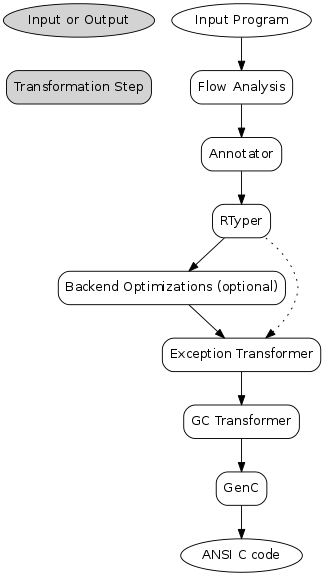
\includegraphics[width=0.5\textwidth]{diagram.png}
\caption{diagram of RPython translation process}
\label{figure-1}
\end{figure}

\section{Γραφήματα Ροής}

\subsection{Τρόπος δημιουργίας}

Ο σκοπός του κατασκευαστή γραφημάτων (υλοποιημένος στο module
\texttt{rpython.flowspace}) είναι να μετατρέψει τα αντικείμενα συναρτήσεων σε
γραφήματα. Κανονικά οι μεταγλωττιστές παίρνουν μια συνάρτηση και την
μετατρέπουν σε ενδιάμεσο bytecode κώδικα σε κάποια εικονική μηχανή (VM) και
έπειτα την τρέχουν. Στο RPython όμως χρησιμοποιείται ένα \textit{abstract
interpretation} το οποίο λειτουργώντας αφαιρετικά μετατρέπει τον ενδιάμεσο
κώδικα στα βασικα \texttt{Block}, τα οποία περιέχουν όλες τις εντολές οι
οποίες επιδρούν πάνω σε αντικείμενα Python. Το αποτέλεσμα της κάθε εντολής
αποθηκεύεται προσωρινά σε μια μεταβλητή η οποία μπορεί να χρησιμοποιηθεί στις
επόμενες. Για ένα παράδειγμα βλ. Σχήμα \ref{figure-2} το οποίο είναι ένα
γράφημα μιας απλής συνάρτησης με ένα if branch. Φαίνεται η γενική εικόνα των
γραφημάτων, το branch καθώς ο τρόπος που επαναχρησιμοποιούνται οι προσωρινές
μεταβλητές αποτελεσμάτων ανάλογα με τις ανάγκες.

\begin{figure}[h]
\centering
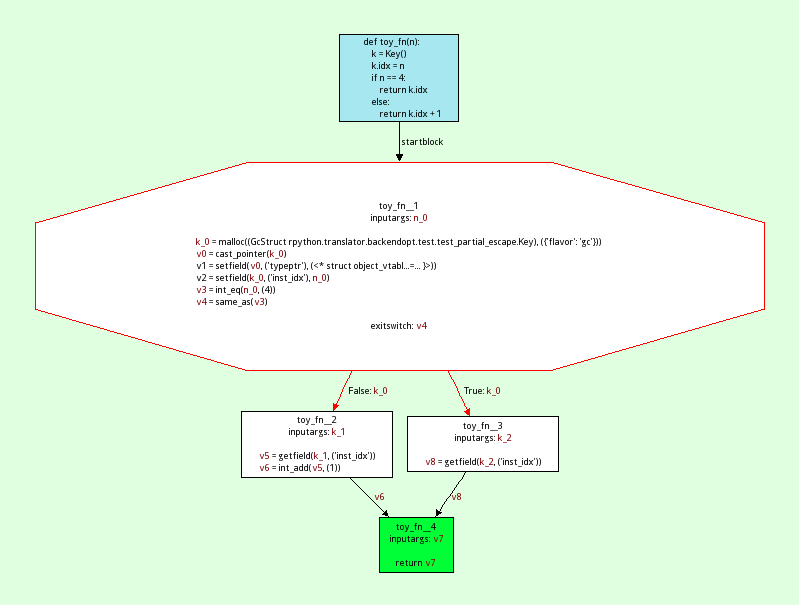
\includegraphics[width=\textwidth]{simple-func-bef.png}
\caption{simple function flow diagram}
\label{figure-2}
\end{figure}

Ο κατασκευαστής ``κλείνει" ένα \texttt{Block} και πάει στο επόμενο σε 2 
περιπτώσεις:

\begin{enumerate}

\item Περίπτωση κλήσης \texttt{is\_true()}. Όταν συμβαίνει αυτό, ο \textit{
abstract interpreter} δεν ξέρει φυσικά αν η συνθήκη θα είναι \textit{True} ή
\textit{False} - αφού η γλώσσα μας είναι δυναμική – οπότε θα πρέπει να τις 
ακολουθήσει και τις 2, δημιουργώντας αντίστοιχα άλλες ροές (δηλαδή
\texttt{Blocks}) για την κάθεμια.

\item Περίπτωση εμφάνισης \textit{joinpoint}. Αυτή η περίπτωση λαμβάνει χώρα
όταν η επόμενη εντολή, που πρόκειται να καταγράψουμε στο τρέχον \texttt{Block},
έχει ήδη καταγραφεί ή καταγράφεται τώρα από άλλο \texttt{Block}. Αυτό σημαίνει
ότι ο μεταγλωττιστής έχει κλείσει κάποιον βρόγχο και πρόκειται να μεταγλωττίσει
κώδικα τον οποίο έχει ήδη ``δει". Τότε ο μεταγλωττιστής σταματά, και
δημιουργείται ένα \texttt{Link} απο το τρέχον \texttt{Block} στο προηγούμενο,
έτσι ώστε να κλείσει ο βρόγχος και στο διάγραμμα και να υπάρχει πιστή
αναπαράσταση του κώδικα.

\end{enumerate}

\subsection{Το μοντέλο}

Η βασική συνάρτηση που δημιουργεί τις δομές δεδομένων που απαρτίζουν το μοντέλο
είναι η \texttt{build\_flow()}. Η μονάδα (unit) ροής είναι το αντικείμενο
\texttt{FunctionGraph} το οποίο μαζί με τα υπόλοιπα (που συνήθως περιέχονται σε
αυτό) ορίζονται στο αρχείο \texttt{rpython/flowspace/model.py}. Τα περιγράφουμε
παρακάτω:

\begin{itemize}

\item \texttt{FunctionGraph} Το διάγραμμα ροής μια συνάρτησης. Είναι η βασική
δομή δεδομένων του μεταγλωττιστή. Περιέχει αναφορές και μια λίστα απο
\texttt{Blocks}, τα οποία συνδέονται με \texttt{Links}. Βασικά κομμάτια του
είναι:

\begin{enumerate}
\item \textbf{startblock:} Το πρώτο block του γραφήματος. Είναι το σημείο
εισόδου για την ροή του προγράμματος όταν αυτή φτάσει σε αυτή την συνάρτηση. Οι
παράμετροι εισόδου θα δοθούν σε αυτό το block. Αυτό το block θα δείχνει όπως
και όλα τα άλλα σε επόμενα ανάλογα με την ροή.
\item \textbf{returnblock:} Το μοναδικό block στο κάθε γράφημα που μπορεί να
εκτελέσει μια ``επιστροφή" της συνάρτησης στην ροή του ανώτερου επίπεδου
(function return). Είναι πάντα άδειο και δεν περιέχει ούτε την εντολής
επιστροφής – αυτή υπονοείται. Τα links δείχνουν εδώ όταν και μόνο όταν θέλουν
να τερματίσουν την συνάρτηση. Η μοναδική παράμετρος είναι η τιμή επιστροφής.
\item \textbf{exceptblock:} Αυτό και το παραπάνω είναι τα μόνα blocks που
μπορούν να τερματίσουν την ροή. Είναι το μοναδικό block που μπορεί να
``πυροδοτήσει" μια εξαίρεση. Δέχεται 2 τιμές· η πρώτη είναι η κλάση της εξαίρεσης
και η δεύτερη η τιμής της. Η μόνη περίπτωση να υπάρχει link προς αυτό το block
είναι η ρητή πυροδότηση εξαίρεσης από το πρόγραμμα.
\end{enumerate}

\item \texttt{Block} Το πιο σημαντικό κομμάτι ενός γραφήματος. Ένα γράφημα
ουσιαστικά είναι μια λίστα από blocks. Ένα block περιέχει μια λίστα από
\texttt{SpaceOperation}s, δηλαδή μια λίστα από εντολές. Λεπτομερειακά
αποτελείται από:

\begin{enumerate}
\item \textbf{inputargs:} Είναι μια λίστα με όλες τις μεταβλητές (με καινούργια
ονόματα) που μπορούν να εισέλθουν στο block από οποιοδήποτε προηγούμενο. Η
αντιστοίχηση των παλιών ονομάτων που υπάρχουν στα links με τα καινούργια 
γίνεται ένα προς ένα (π.χ. η πρώτη στα link με την πρώτη στη λίστα).
\item \textbf{operations:} Η λίστα με τις εντολές που θα τρέξουν όταν η ροή
καταλήξει σε αυτό το block. Θα τρέξουν όλες σειριακά χωρίς εξαιρέσεις. Οι
εντολές υποδεικνύονται από \texttt{SpaceOperation}s (βλ. πιο κάτω).
\item \textbf{exits:} Λίστα με πιθανά \textit{άλματα} (jumps). Φυσικά περιέχει
links. Σε ``συνεργασία" με το επόμενο μέλος καθορίζει που θα προχωρήσει η ροή 
του προγράμματος. Φυσικά περιέχει ένα ή περισσότερα links.
\item \textbf{exitswitch:} Τα περιεχόμενα αυτού του μέλους ποικίλλουν:

\begin{enumerate}
\item Δεν υπάρχει \textit{jump} και περιέχει \texttt{None}. Το \textit{exits}
περιέχει ένα link.
\item Άλμα υπό συνθήκη. Σε αυτή την περίπτωση το \textit{exitswitch} είναι μια
από τις μεταβλητές του block. Σε συνεργασία με ένα αντίστοιχο
\textit{exitcase} στα \texttt{Link}s, διευθετεί τις περιπτώσεις των branches.
Η ροή θα ακολουθήσει το \texttt{Link}, του οποίου το \textit{exitcase},
ταιριάζει με το \textit{exitswitch} του \texttt{Block}. Αν δεν υπάρχει 
ταίριασμα τότε έχουμε runtime error.
\item Εξαίρεση. Το \textit{exitswitch} περιέχει
\texttt{Constant(last\_exception)}. Το πρώτο \texttt{Link} του \textit{exits}
περιέχει \texttt{None} στο \textit{exitcase} του για την περίπτωση που δεν
υπάρχει εξαίρεση. Τα υπόλοιπα links δείχνουν στα διάφορα classes των εξαιρέσεων
και ακολουθούνται αντίστοιχα. Φυσικά με αυτόν τον τρόπο ``προστατεύτεται" μόνο η
τελευταία εντολή.
\item Επιστροφή. Περίπτωση \textit{Returnblock}. Το \textit{exitswitch}
και το \textit{operations} είναι άδεια και το \textit{exits} είναι ρυθμισμένο 
σε \texttt{None}.
\end{enumerate}

\end{enumerate}

\item \texttt{Link} Αποτελεί την σύνδεση μεταξύ των Blocks. Περιέχει:

\begin{enumerate}
\item \textbf{prevblock:} Το προηγούμενο \texttt{Block} από το οποίο δείχνει 
αυτό το \texttt{Link}.
\item \textbf{target:} Το \texttt{Block} στο οποίο δείχνει. Μπορεί να είναι 
μόνο ένα. Αν το \texttt{Block} πρέπει να δείξει σε περισσότερα, τότε πρέπει να 
υπάρχουν πολλά \texttt{Link}s.
\item \textbf{args:} Λίστα με \texttt{Variable}s και \texttt{Constant}s. Βλ. 
παραπάνω.
\item \textbf{exitcase:} Βλ. παραπάνω.
\item \textbf{last\_exception:} Εδώ θα τοποθετηθεί (στο runtime) η κλάση 
εξαίρεσης σε τέτοια περίπτωση, αν το \texttt{Link} δείχνει σε \texttt{Block} 
εξαιρέσεων.
\item \textbf{last\_exc\_value:} Ομοίως εδώ θα τοποθετηθεί η τιμή.
\end{enumerate}

\item \texttt{SpaceOperation} Υποδεικνύει μια ``εντολή". Είτε καταγεγραμμένη 
είτε δημιουργημένη από τον ίδιο τον μεταφραστή. Σε αυτό το σημείο οι εντολές 
είναι σχετικά περιορισμένες (λ.χ. δεν μπορούν να πυροδοτήσουν μια εξαίρεση).
Αυτό σημαίνει ότι ο μεταφραστής μπορεί να υποθέσει ότι είναι ασφαλείς και να
εκτελέσει ενεργειες (όπως ανάγνωση μνήμης) που σε άλλες περιπτώσεις θα
απαιτούσαν π.χ. locking. Υπάρχουν 2 πιθανές εξαιρέσεις σε αυτό το σενάριο.

\begin{itemize}
\item η περίπτωση κλήσης άλλης συνάρτησης (βλ. \texttt{simple\_call()})
\item η τελευταία εντολή σε ένα \texttt{Block} χειρισμού εξαιρέσεων μπορεί να
μην είναι ασφαλής.
\end{itemize}

Περιέχει:

\begin{enumerate}

\item \textbf{opname:} Το όνομα της εντολής. Η λίστα με τις εντόλες βρίσκεται 
στο αρχείο \texttt{rpython.flowspace.operation}.
\item \textbf{args:} Τα ορίσματα της εντολής. Μπορεί να είναι \texttt{Constant}
ή \texttt{Variable} αλλά να περιέχεται στο Block.
\item \textbf{result:} καινούργια μεταβλητή στην οποία θα αποθηκευτεί το 
αποτέλεσμα.
\end{enumerate}

\item \texttt{Variable} Αποτελεί ένα placeholder και θα αποκτήσει τιμή κατά το
runtime. Μπορεί προφανώς να είναι όρισμα σε κάποια εντολή. Περιέχονται κάποια 
μέλη με σκοπούς debugging.

\begin{enumerate}
\item \textbf{name:} Εγγυημένα μοναδικό όνομα. Δεν ταιριάζει φυσικά με το 
όνομα που έχει η μεταβλητή στον κώδικα του χρήστη.
\end{enumerate}

\item \texttt{Constant} Αποτελεί την αναπαράσταση μιας σταθεράς. Όπως και 
παραπάνω μπορεί να είναι όρισμα σε κάποια εντολή, ή να βρίσκεται στην λίστα 
κάποιου Link για την αρχικοποίηση των μεταβλητών του επόμενου Block.

\begin{enumerate}
\item \textbf{value:}
\item \textbf{key:} hashed\footnote{βλ. hash function} αντικείμενο που 
αντιπροσωπεύει την τιμή του \textit{value}, για λόγους ασφάλειας κ.α.
\end{enumerate}

\end{itemize}

\section{Πέρασμα Υποσημειώσεων – Annotation Pass}

Αυτό το υποσύστημα ``υποσημειώνει" τα γραφήματα με ειδικές πληροφορίες
(υπογραφές) έτσι ώστε τα επόμενα υποσυστήματα να γνωρίζουν τους εκάστοτε τύπους
των μεταβλητών και των αντικειμένων. Μπορούμε να πούμε ότι είναι ένα είδος
\textit{type inference}. Μία από αυτές τις υπογραφές για τις μεταβλητές, που θα
υποσημειωθούν, θα περιγράφει όλους τις πιθανούς τύπους που θα είναι δυνατόν να
περιέχει η μεταβλητή αυτή κατά την διάρκεια του runtime. Η ανάλυση/πέρασμα
γίνεται ανά συνάρτηση-γράφημα. Το αποτέλεσμα είναι ένα μεγάλο dictionary που
``δείχνει" από μεταβλητές σε τέτοιες υπογραφές.

Η υπογραφή είναι ένα ``στιγμιότυπο" (\textit{instance}) μιας υποκλάσης ενός
\texttt{SomeObject} αντικειμένου. Κάθε υποκλάση αντιπροσωπεύει και μια άλλη
οικογένεια αντικειμένων. Η κλάση βάσης, όπως είπαμε, είναι η
\texttt{SomeObject}, η οποία αντιπροσωπεύει ένα αντικείμενο Python. Υποκλάσεις
της είναι – μεταξύ άλλων – οι: \texttt{SomeInteger()} (με την επιλογή
\texttt{nonneg=True} ανάλογα άν χρειάζονται αρνητικοί αριθμοί),
\texttt{SomeString()}, \texttt{SomeChar()} και \texttt{SomeTuple()}, οι οποίοι
αντιπροσωπεύουν τα προφανή αντικείμενα. Να σημειώσουμε εδώ ότι όλα τα παραπάνω 
αντικείμενα υπογραφών είναι αμετάβλητα, δηλαδή δεν αλλάζουν \textit{in-place}. 
Αυτό σημαίνει ότι εάν ο Annotator αποφασίσει να αλλάξει την υπογραφή, θα 
πρέπει να δημιουργήσει ένα καινούργιο αντικείμενο.

Υπάρχουν αντικείμενα βέβαια τα οποία είναι μεταβλητά, καθώς και αυτά που
αντιπροσωπεύουν χρήζουν προσοχής και ειδικής μεταχείρησης. Σε αυτά, οι 
πληροφορίες μεταβάλλονται καθ όλη την διάρκεια του annotation pass.
Περιλαμβάνουν το \texttt{SomeList()} και το \texttt{SomeDict()}.

Οι πιο εξειδικευμένες περιπτώσεις έχουν να κάνουν με κλάσεις ορισμένες από τον
χρήστη (\textit{user-defined classes}). Το σύστημα τις διαχειρίζεται με το
\texttt{SomeInstance}. Για κάθε τέτοια κλάση διατηρούμε ένα \textit{ClassDef},
που ουσιαστικά περιέχει τα ορίσματα και τα στοιχεία (attibutes) της κλάσης αυτής
σε επίπεδο ορίσματος (class level attibutes) και στιγμιότυπου (instance level
attibutes). Τα τελευταία ``ανακαλύπτονται" προοδευτικά καθώς ο μεταγλωττιστής
προχωρεί κατά μήκος του κώδικα. Για παράδειγμα, το παρακάτω θα μεταβάλει το
\textit{ClassDef} του στιγμιότυπου με το attribute.

\begin{verbatim}
inst.attr = value
\end{verbatim}

Η διαφορές μεταξύ των επιπέδων class και των instance είναι λίγες και λεπτές.
Γενικά τα attibutes των class-level χρησιμοποιούνται ως αρχικοποιητές για τα
αντίστοιχα των instance-level\footnote{Το ίδιο ισχύει και για (μεταβλητές που
περιέχουν) συναρτήσεις.}. Για κάθε attribute σημειώνονται οι θέσεις που
λαμβάνουν χώρα αναγνώσεις και έπειτα, κατά την ανάλυση, αν υπάρχει γενικοποίηση
του attribute για κάποιο λόγο, ο μεταγλωττιστής επιστρέφει σε αυτά τα σημεία και
τα μεταβάλει ανάλογα, κάνοντάς τα \textit{valid} ξανά.

\section{RTyper}

Ο RTyper είναι μια γέφυρα μεταξύ του Annotator και των παραγωγών κώδικα. Είναι
απαραίτητος γιατί ο Annotator υποσημειώνει τον κώδικα με \textit{υπογραφές}
τύπων είτε δημιουργημένους από τον χρήση\footnote{user-defined classes} είτε
πολύ κοντά στο υψηλό επίπεδο της RPython. Οπότε – για να μπορούμε να παράγουμε
κώδικα – απαιτείται η υποσημείωση των γραφημάτων για το επίπεδο της γλώσσας
στόχου, δηλαδή χαμηλού επιπέδου με δείκτες και arrays. Ο RTyper αναλαμβάνει να
αποφανθεί για τον τύπο και να αντικαταστήσει τις εντολές υψηλού επιπέδου με
άλλες αντίστοιχες χαμηλότερου επιπέδου στα γραφήματα. Προφανώς η αντιστοιχία
δεν είναι 1 προς 1, και μερικές φορές απαιτούνται πολύ περισσότερες εντολές στο
χαμηλό επίπεδο για να μιμηθούμε τις αντίστοιχες του υψηλού. Επιπλέον οι
διαθέσιμες εντολές και οι τύποι είναι σαφώς περιορισμένοι. Τελος, πρέπει να
σημειωθεί ότι αυτό το βήμα θα μπορούσε να μην γίνει, αλλά οι σχεδιαστές έχουν
επιλέξει να είναι ένα αυτόνομο module του συστήματος έτσι ώστε να κάνει την
δουλεία του παραγωγού κώδικα πιο εύκολη και πιο αποδοτική. Μετά το πέρασμα του
RTyper η παραγωγή κώδικα είναι σχετικά τετριμμένη.

%%%%%%%%%%%%%%%%%%%%%%%%%%%%%%%%%%%%%%%%%%%%%%%%%%%%

\section{Προετοιμασία}

\subsection{Διαχείριση Μνήμης}

Αφού η Python είναι δυναμική ενώ οι περισσότερες από τις γλώσσες παραγωγών
(compiled target languages) δεν είναι· θα πρέπει το σύστημα να κάνει κάποιες
επιλογές για την διαχείριση της μνήμης. Αυτές οι επιλογές είναι εξαιρετικά
σημαντικές για την τελική ταχύτητα των προγραμμάτων καθώς γενικά ο κώδικας
Python τείνει να δεσμεύει μνήμη με πολύ γρήγορους ρυθμούς. Το σύστημα είναι
ευέλικτο και υπάρχουν πολλές επιλογές. Δεν θα μπούμε σε επιπλέον πληροφορίες
γιατί είναι έξω από τα όρια σκοπού της εργασίας αυτής, αλλά πληροφοριακά
υπάρχουν:

\begin{itemize}
\item reference counting (απαρχαιωμένο – δεν χρησιμοποιείται πλέον στο σύστημα)
\item ένας συντηρητικός BDW (B\``ohm-Demers-Weiser) συλλέκτης\cite{bdw}
\item πλέον χρησιμοποιούνται άλλοι custom συλλέκτες (βλ. \cite{gc}).
\end{itemize}

\subsection{Διαχείριση Εξαιρέσεων}

Ο κώδικας RPython υποστηρίζει πλήρως συντακτικό εξαιρέσεων ακριβώς όπως και η
κανονική Python. Όπως και πριν βέβαια οι γλώσσες παραγωγών δεν "γνωρίζουν`` την
έννοια των εξαιρέσεων οπότε ο απαραίτητος κώδικας διαχείρισης θα πρέπει να
προστεθεί. Το σύστημα δουλεύει όπως το κανονικό σύστημα της Python στον
μεταγλωττιστή CPython: οι εξαιρέσεις υποδεικνύονται με ειδικές τιμές επιστροφής
(return values) και η τρέχουσα εξαίρεση αποθηκεύεται σε μια καθολική (global)
δομή δεδομένων, ορατή από όλα τα πεδία δράσης (scope) του προγράμματος.


\chapter{Θεωρία Μερικής Ανάλυσης Διαφυγής}
\label{chapter3b} 

\section{Εισαγωγικά}

Αρχικά να σημειώσουμε, ότι η Θεωρία που παραθέτουμε εδώ είναι βασισμένη κυρίως
στο paper των W{\"u}rthinger et al\cite{stadler2014partial} αλλά και σε επιπλέον
έρευνα και εμπειρία που αποκτήσαμε κατά την υλοποίηση του module. Η μέθοδος,
λοιπόν, που θα προσπαθίσουμε να υλοποιήσουμε στο module μας λέγεται
\textit{Μερική Ανάλυση Διαφυγής} (\textit{Partial Escape Analysis}) και είναι
μια γενίκευση της κανονικής ``Απλής" Ανάλυσης Διαφυγής. Σκοπός μας είναι προφανώς
η βελτιστοποίηση των προγραμμάτων και για να το πετύχουμε αυτό στοχεύουμε στο να
μειώσουμε τον αριθμό των μεταβλητών που χρησιμοποιεί ο χρήστης, και τον αριθμό
των προσβάσεων (\textit{accesses}) που κάνει στην μνήμη για αυτές.

Η πιο προφανής βελτιστοποίηση με βάση αυτή την ανάλυση είναι η πλήρης εξάλειψη
των δεικτών που δεν διαφεύγουν ή η αντικατάστασή τους με βαθμωτούς μέσα στο
δυναμικό τους πεδίο. Επίσης δυνατή είναι η αντικατάσταση καταχωρήσεων μνήμης
(malloc) στον σωρό (heap) με απλές κατωχηρώσεις στη στοίβα (stack) πράγμα που
κάνει το πρόγραμμα πολύ πιο γρήγορο, και στην περίπτωση γλώσσας με σύστημα
``συλλογής απορριμμάτων" αυτό οδηγεί στο τρέξιμο του συλλέκτη λιγότερες φορές.
Τέλος μπορούμε να έχουμε κάποια οφέλη στα συστήματα συγχρονισμού. Αν ο δείκτης
βρεθεί να μπορεί να προσπελαστεί μόνο από ένα νήμα, τότε μπορούμε να 
αφαιρέσουμε τις δομές συγχρονισμού. Εμείς θα ασχοληθούμε μόνο με αντικατάσταση 
βαθμωτών.

Να αναφέρουμε εδώ ότι μέχρι την στιγμή που γράφονται αυτές οι γραμμές, η
στρατηγική που ακολουθεί το paper για τα loops δεν έχει υλοποιηθεί. Για την
ακρίβεια δεν έχει υλοποιηθεί καμία στρατηγική για τα loops, και απλά αγνoούμε
την ``ιδιότητα" που έχουν να επιστρέφουν την ροή της εκτέλεσης προς τα πίσω.
Εχουμε λάβει υπόψιν μας την μη γραμμική ροή σε περίπτωση ύπαρξης \textit{jump
back} στο γράφημα – aka: \textit{loop} αλλά δεν έχουμε τρόπο ανάλυσης των
εσωτερικών μεταβλητών και αντικειμένων. Όταν εντοπιστεί \textit{loop}, τότε
\textit{επανατοποθετούνται} όλα τα εικονικά αντικέιμενα. Θα δούμε τι σημαίνουν
οι παραπάνω παράξενοι ίσως όροι παρακάτω. Κανονική υλοποίηση του \textit{loop
handling} συμπεριλαμβάνεται στις μελλοντικές εργασίες. Η υλοποίηση δεν έγινε
γιατί κρίναμε ``βαρύ" και ``ακριβό"\footnote{αν όχι λανθασμένο} το
\textit{approach} – την στρατηγική που παραθέτεται: Αυτό που πρότεινε το paper
ήταν ένα είδος \textit{testing} του \textit{escapability} των εσωτερικών
αντικειμένων που χρησιμοποιούνται στο loop, και η ``ανάκληση" όλων των ενεργειών
(\textit{reverse}) σε περίπτωση που στο τέλος κριθεί μη αποδοτική ή λανθασμένης
λογικής.

Μια ανάλυση της πολυπλοκότητάς της δίνεται εδώ\cite{complexity} και επιπλέον
παραθέτουμε εμείς κάποιες λεπτομέρειες σε επόμενη παράγραφο.

%------------------------------------------------------------------------------

\section{Η Απλή Ανάλυση}

Για να πετύχουμε τα παραπάνω αρκεί να ``αναλύσουμε" τις μεταβλητές μια-μια και να
καθορίσουμε όλα τα μέρη όπου μια μεταβλητή απαιτείται να υπάρχει καθώς επίσης
και το αν η διάρκεια ζωής της μπορεί να αποδειχθεί να περιορίζεται μόνο στην
τρέχουσα διαδικασία και/ή νήμα\footnote{\textit{thread}}, δηλαδή το
\textit{scope}. Με τον όρο μεταβλητή εδώ εννοούμε ένας δείκτης σε μια θέση
μνήμης. Χρησιμοποιούμε τους όρους ``μεταβλητή" και ``δέικτης" εναλλακτικά.

Με άλλα λόγια, η \textit{Ανάλυση Διαφυγής} είναι μια μέθοδος για τον καθορισμό
του \textit{δυναμικού πεδίου} των δεικτών ενός προγράμματος. Την περιοχή δηλαδή,
στην οποία οι δείκτες αυτοί είναι ενεργοί και έγκυροι ή αλλιώς την περιοχή που
μπορεί το πρόγραμμα να έχει ``πρόσβαση" σε αυτούς. Πιο συγκεκριμένα η
\textit{Ανάλυση Διαφυγής} ελέγχει εάν ένα (δεσμευμένο από το σύστημα)
αντικείμενο \textit{διαφεύγει} από αυτό το scope.

Ένας δείκτης που δημιουργείται από κάποια συνάρτηση – δηλαδή ένα
\textit{reference} σε ένα αντικείμενο (της Python) – μπορεί να \textit{διαφύγει}
σε κάποια άλλη. Τότε το δυναμικό του πεδίο μεγαλώνει. Ένας δείκτης λέμε ότι έχει
\textit{διαφύγει} όταν αυτός είναι διαθέσιμος (ή αλλιώς ορατός) και από άλλα
scopes στο πρόγραμμα, οπότε \textbf{απαιτείται} να υπάρχει αυτός καθ'αυτός. Ο
σημαντικότερος τρόπος για διαφυγή είναι η επιστροφή του αντικειμένου ως return
value μιας συνάρτησης. Θα δούμε αναλυτικά και άλλους τρόπους στο επόμενο
κεφάλαιο απλά να σημειώσουμε ότι υπάρχουν και άλλοι πιο περίπλοκοι τρόποι
διαφυγής όπως στην περίπτωση functional γλωσσών και tail-call optimization, όμως
δε θα ασχοληθούμε με αυτές σε αυτή την εργασία.

Ως ιστορική σημείωση να πούμε ότι παλαιότερα οι μέθοδοι αναλύσης διαφυγής
χρησιμοποιούσαν αλγόριθμους που ονομάζονται ``Equi-Escape
Sets"\cite{kotzmann2005escape} για να αποφανθούν εάν τα αντικείμενα διαφεύγουν
του τρέχοντος scope. Δημιουργούσαν σύνολα (sets) από αντικείμενα που ανήκουν
στην ίδια κατηγορία διαφυγής, έπειτα με το να αναλύουν τις μεθόδους και τις
συναρτήσεις, μπορούσαν να μαρκάρουν τα διάφορα αντικείμενα και σύνολα (π.χ. αν
το αντικείμενο από το ένα σύνολο αναθέτονταν σε ένα άλλο σύνολο) και να τα
συγχωνεύσουν.\cite{stadler2014partial}

Τα αποτελέσματα που θα επιστρέψουμε θα χρησιμοποιηθούν για να τροποποιηθεί ο
κώδικας με βέλτιστο τρόπο. Παρακάτω θα παραθέσουμε ένα παράδειγμα για τον τρόπο
με τον οποίο ο βελτιστοποιητής μας θα μετατρέψει ένα κομμάτι κώδικα. Να
υπογραμμίσουμε εδώ ότι το παράδειγμα είναι από το paper, τροποποιημένο όμως με
τέτοιο τρόπο έτσι ώστε να είναι σχεδιασμένο φυσικά για Python και να αναδεικνύει
τις δυνατότητες και λεπτομέρειες της γλώσσας.

\begin{lstlisting}[language=Python]
class Key(object):
    def __init__(self, idx, ref):
        self.idx = idx
        self.ref = ref
    def equals(self, other):
        return (self.idx == other.idx && self.ref == other.ref)

def createValue(...):
    ...
        
cacheKey = None
cacheValue = None

def getValue(idx, ref):
    key = Key(idx, ref)
    if key.equals(cachekey):
        return cacheValue
    else:
        return createValue(...)
\end{lstlisting}

Το παραπάνω κομμάτι (μετά από ανάλυση διαφυγής και inlining – που εφαρμόζεται
από το PyPy) θα γίνει κάπως έτσι:

\begin{lstlisting}[language=Python]
...
def getValue(idx, ref):
    idx1 = idx
    ref1 = ref
    tmp = cacheKey
    if (idx1 == tmp.idx && ref1 == tmp.ref):
        return cacheValue
    else:
        return createValue(...);
...

\end{lstlisting}

Αυτό που θα αλλάξει εδώ είναι η συνάρτηση \texttt{getValue()} κατά το
compilation της. Όταν ο μεταγλωττιστής φτάσει σε αυτή, θα καταλήξει στο
συμπέρασμα ότι κανένα reference στο δεσμευμένο αντικείμενο \texttt{Key} δεν
διαφεύγει από το τρέχων compilation scope της συνάρτησης. Αυτό σημαίνει ότι
κανένα reference δεν θα υπάρχει αφού τερματίσει και επιστρέψει η συνάρτηση και
ότι κανένα άλλο αντικείμενο ή κατασκευή ή συνάρτηση δεν θα ``θέλει" να αναφερθεί
σε αυτό. Οπότε, μπορούμε να τροποποιήσουμε τον κώδικα με τους παρακάτω τρόπους:

\begin{itemize}

\item Η δέσμευση μνήμης του αντικειμένου στον σωρό (\textit{garbage collected
heap}) μπορεί να αντικατασταθεί με μια απλή δέσμευση στην στοίβα
(\textit{stack}) της συνάρτησης ή σε κάποια άλλη περιοχή ή ζώνη\footnote{Ζώνες
ονομάζονται περιοχές του σωρού (heap) που έχουν ήδη αρχικοποιηθεί και έχουν
περιορισμένη διάρκεια ζωής με σκοπό αυτό ακριβώς το είδος χρήσης.} η οποία δεν
υπόκειται συλλογή απορριμάτων. Αυτό σημαίνει ότι μια κανονική δέσμευση (με την
εντολή \textit{malloc}), που θα έχει μεγάλη διάρκεια ζωής και θα είναι ακριβή
και στην αρχικοποίηση και στον καθαρισμό της, μπορεί να μεταβληθεί σε μια απλή
προσωρινή μεταβλητή στην συνάρτηση που μετά το πέρας του runtime της, θα
ελευθερωθεί. Αυτό μας εξοικονομεί και χρόνο (σε δύο περιπτώσεις –
\textit{allocation} και \textit{freeing}) και μνήμη.

\item \textit{Αντικατάσταση Βαθμωτών} Εκτός από το παραπάνω μπορούμε
να προχωρήσουμε σε αντικατάσταση με βαθμωτούς. Αυτό θα εξαλείψει τελείως την
δέσμευση, με το να αντικαταστήσει τα fields του αντικειμένου με τοπικές
μεταβλητές.

\end{itemize}

Βλέπουμε ότι η δέσμευση του αντικειμένου \texttt{Key} αντικαταστήθηκε με τις
τοπικές μεταβλητές \texttt{idx1} και \texttt{ref1}. Αν και αυτό είναι
εξιδανικευμένο παράδειγμα, μπορούμε να περιμένουμε πολλές τέτοιες βελτιώσεις
ακόμα και σε \textit{real-world} κομμάτια κώδικα και βιβλιοθήκες, όπως θα δούμε
στο τελευταίο κεφάλαιο.

Επίσης σημαντική αλλαγή είναι το inlining που πραγματοποιήθηκε στον κώδικα, και
αυτό ήταν ζωτικό στο να μπορέσει η ανάλυσή μας να ``εξάγει" το σωστό αποτέλεσμα
για τις μεταβλητές. Σε αντίθετη περίπτωση η ``μονή" χρήση του αντικειμένου (του
\texttt{Key}) θα είχε ουσιαστικά κρυφτεί πίσω από μια κλήση στην μέθοδο του
αντικειμένου.

Σημειώνουμε ότι  το παραπάνω είναι κανονικός κώδικας Python – ελλιπής βέβαια και
δεν μπορεί να τρέξει – για παιδαγωγικούς σκοπούς. Για παράδειγμα δεν παραθέτουμε
τον ορισμό της συνάρτηση \texttt{createValue()} που προφανώς είναι η ``ακριβή"
συνάρτηση που δημιουργεί το αντικείμενο που θέλουμε να αποφύγουμε (βλ. γραμμές
8-9 και 19). Όσων αφορά το δεύτερο βελτιστοποιημένο κομμάτι, δεν παραθέτουμε
καθόλου την κλάση \texttt{Key()} και δεν δίνουμε το τι περιέχουν οι καθολικές
μεταβλητές (βλ. γραμμή 5). Ο αναγνώστης αρκεί να ξέρει ότι προσπαθούμε να
αποφύγουμε την δέσμευση και χρήση μνήμης. Να υπογραμμίσουμε επίσης ότι, στην
πραγματικότητα ο βελτιστοποιητής μας δεν αλλάζει – ούτε παράγει – κώδικα Python,
αλλά middleware κώδικα, και δουλεύει πάνω σε διαγράμματα ροής όπως θα δούμε στα
επόμενα κεφάλαια.

Τέλος να πούμε ότι η απλή ανάλυση διαφυγής είναι ήδη υλοποιημένη στο PyPy στο
αρχείο \texttt{escape.py}, και χρησιμοποιείται κανονικά και αποδοτικά στο
compiling του ίδιου του μεταγλωττιστή καθώς και άλλων προγραμμάτων. Στοχεύουμε
σε τέτοιου intergration του module μας στο σύστημα.

%------------------------------------------------------------------------------

\section{Η Μερική Ανάλυση}

Η ``Μερική Ανάλυση Διαφυγής" δουλεύει ομοίως με παραπάνω, αλλά είναι πιο ισχυρή
με την έννοια ότι λαμβάνει υπόψιν της και τα διάφορα παρακλάδια (branches) της
ροής εκτέλεσης κατά την ανάλυση. Με άλλα λόγια η κανονική Ανάλυση Διαφυγής
χειρίζεται μια περίπτωση \texttt{if} ``στατικά" – ουσιαστικά την αγνοεί, ενώ η
αντίστοιχη μερική ακολουθεί και τις 2 πιθανές ροές. Το γεγονός αυτό όμως
καθιστά την σχεδίαση της υλοποίησης πιο δύσκολη.

Σε πολλές περιπτώσεις το γεγονός ότι η απλή ανάλυση αγνοεί τα \textit{if splits}
και απλά παίρνει καθολικές αποφάσεις, οδηγεί στην ανικανότητα να ανιχνευτεί η
δυνατότητα αφαίρεσης κάποιων αντικειμένων. Για αυτό τον λόγο η μερική ανάλυση, η
οποία μπαίνει στο κάθε branch και το αναλύει ξεχωριστά, θεωρείται ισχυρότερη.
Διατρέχει τον κώδικα με τον ίδιο τρόπο όπως η απλή ανάλυση αλλά διατηρεί
``καταστάσεις" (states) για κάθε branch που έχει γίνει στην ροή και όταν τα
branches συγκλίνουν ξανά, μπορεί να αποφασίσει αν το αντικείμενο διαφεύγει
ανάλογα με το τι συνέβη στο κάθε ένα από αυτά. Οι αποφάσεις αυτές λαμβάνουν χώρα
και για κάθε state ξεχωριστά αλλά το ένα επηρεάζει το άλλο αφού φυσικά ο
μεταγλωττιστής δεν μπορεί να ξέρει ποιο από τα branches θα ακολουθηθεί
πραγματικά.

Όλα τα επόμενα κεφάλαια απο τώρα και στο εξής αναφέρονται στην μερίκη ανάλυση
διαφυγής. Στο επόμενο υποκεφάλαιο, αφού πρώτα συζητήσουμε για την πολυπλοκότητα
της μεθόδου, Θα συνεχίσουμε με κάποιες λεπτομέρειες για τον τρόπο που δουλεύει η
μερική ανάλυση προκειμένου να εγκλιματιστεί ο αναγνώστης και έπειτα θα δώσουμε
ένα εκτενές παράδειγμα με όλες τις λεπτομέριες που θα μπορούν τότε να
κατανοηθούν καλύτερα.

\section{Πολυπλοκότητες}

Στο paper που βασιζόμαστε\cite{stadler2014partial} δεν γίνεται καμία αναφορά
στην πολυπλοκότητα της μεθόδου είτε της απλής είτε της μερικής ανάλυσης
διαφυγής. Εμείς θα αποπειραθούμε να δώσουμε μια πρόβλεψη αν και θα
παραλείψουμε τυχών αποδείξεις καθώς είναι εκτός του scope της εργασίας. Στην
καλύτερη περίπτωση (\textit{best case scenario} – BCS) η πολυπλοκότητα
προφανώς περιορίζεται στον αριθμό των operations δήλαδή $O(operations)$, αφού
δεν γίνονται καθόλου αλλαγές και οι εντολές απλά ``αγγίζονται" όλες μια φορά.
Παράδειγμα ένα πάρα πολύ απλό πρόγραμμα χωρίς \textit{if} που επιστρέφει μια
σταθερά και όχι ένα αντικείμενο. Από την άλλη στην χειρότερη περίπτωση
(\textit{worst case scenario} – WCS) η πολυπλοκότητά μας ανεβαίνει στο
επίπεδο:
\[
O(operations \times blocks)
\]
αφού θα πρέπει όλες οι εντολές να αφαιρεθούν και να ξανατοποθετηθούν στα επόμενα
\texttt{Block}s. Ως παράδειγμα να αναφέρουμε την περίπτωση όπου έχουμε μια
εντολή \texttt{malloc} και αμέσως μετά ένα \textit{split} με χιλιάδες branched-
off \textit{Block}s. Σε αυτή την περίπτωση η \texttt{malloc} θα πρέπει να
επανατοποθετηθεί (ή να τεσταριστεί αν πρέπει να επανατοποθετηθεί) τόσες φορές
όσες και τα \textit{Block}s. Βέβαια η πολυπλοκότητα μένει σαφώς στην ίδια τάξη
μεγέθους οπότε η μέση περίπτωση (\textit{average case scenario} – ACS) είναι
ίδια.

Τα παραπάνω ισχύουν για την στρατηγική που ακολουθούμε εμείς. Η στρατηγική του
paper είναι ίδια με την διαφορά του χαρακτηριστικού της υλοποίησής τους για τα
loops. Εμείς, όπως είπαμε παραπάνω, ουσιαστικά αγνοούμε τα loops. Στο paper οι
συγγραφείς προτείνουν μια μέθοδο ``testing" και ``reversing" σε περίπτωση λάθους.
Αυτό όμως είναι εξαιρετικά μη αποδοτικό καθώς σίγουρα θα υπάρχει η περίπτωση
επανατοποθέτησης και μετά ανάγκη αναίρεσης οπότε στην χειρότερη περίπτωση (WCS)
η πολυπλοκότητα ανεβαίνει τάξη μεγέθους και γίνεται τετραγωνική (quadratic
factor).

%------------------------------------------------------------------------------

\section{Τρόπος λειτουργείας – Λεπτομέρειες} % make subsubsections?

\subsection{Γενικά}

Η βελτιστοποίηση αυτή θα κρίνει ποιες μεταβλητές είναι απαραίτητο να υπάρχουν
αυτές καθ' αυτές (ίσως γιατί βασίζεται κάποιος εξωτερικός παράγωντας σε αυτές)
και θα αποπειραθεί να αφαιρέσει τις υπόλοιπες. Η αφαίρεση αυτή θα πρέπει φυσικά
να είναι έξυπνη καθώς η λειτουργία και η ορθότητα του προγράμματος θα πρέπει
προφανώς να διατηρηθούν.

Οι 2 κυριότεροι λόγοι για να απαιτείται η ύπαρξη της μεταβλητής είναι:
\begin{enumerate}
\item η χρήση της ως τιμή επιστροφής από την συνάρτηση (\textit{return})
\item η αλλαγή του scope της (\textit{globalization})
\end{enumerate} 

\subsection{Τρόπος ανάλυσης \& δομές δεδομένων}

Γενικά η μέθοδος, που περιγράφεται στο paper που ακολουθούμε
\cite{stadler2014partial} και θα υλοποιήσουμε εμείς, σκανάρει το πρόγραμμα και
``παρακολουθεί" τις μεταβλητές και τις κατασκευές του προγραμματιστή. Ξεκινά
σειριακά ακολουθόντας την ροή της εκτέλεσης στο κάθε γράφημα – αφού είναι graph-
based – από ένα ειδικό Block που είναι το πρώτο (\textit{startblock}). Η σειρά
που θα ακολουθήσει στα \texttt{Block}s είναι φυσικά η σειρά της ροής πηγαίνοντας
από πατέρα σε παιδί/παιδιά, ανοίγοντας καταλλήλως ανάλογα με τα \textit{splits}
και τα \textit{merges}. To \textit{merging} γίνεται στα ειδικά \texttt{Block}s
που λέγονται \textit{mergeblocks} όπως θα δούμε παρακάτω. Η ανάλυση αυτή σταματά
όταν φτάσουμε σε κάτι που αποκαλείται \textit{control sink}. Αυτό είναι συνήθως
κάποιο \texttt{Return Block} αλλά μπορεί να έιναι και \texttt{Throw Block} – το
τελευταίο συμπεριφέρεται με τον ίδιο τρόπο με ένα \texttt{Return Block} και
εσωτερικά είναι ομοίως υλοποιημένο.

Καθώς γίνεται αυτό το παραπάνω πέρασμα μια φορά από κάθε \texttt{Block},
διατηρούμε κάποιες πληροφορίες για τις μεταβλητές ανάλογα με την εντολή
(operation) που θα συναντήσει ο μεταγλωττιστής στο εκάστοτε \texttt{Block}. Εδώ
να πούμε ότι οι εντολές είναι αυστηρά σειριακές μέσα σε κάθε \texttt{Block} από
την φύση των γραφημάτων. Αυτός είναι και ο τρόπος που τις συναντά λοιπόν ο
μεταγλωττιστής, χωρίς εμείς να χρειαστεί να κάνουμε κάτι συγκεκριμένο όπως στην
περίπτωση της σειράς επεξεργασίας των \texttt{Block}s. Όλα γίνονται αυτόματα από
το σύστημα των γραφημάτων του PyPy.

Η βασική δομή που χρησιμοποιούμε είναι τα ``εικονικά αντικείμενα"
(\textit{VirtualObjects}). H χρήση τους έγκειται στη αναπαράσταση των πιθανών
μεταβλητών που μπορεί να είναι ``υποψήφιες" για αφαίρεση (αντικατάσταση με
βαθμωτούς).

Ο μεταγλωττιστής, για κάθε καινούργια μεταβλητή που συναντά, δημιουργεί και
διατηρεί ένα τέτοιο εικονικό αντικείμενο, και διαγράφει την ακριβή (σε χρόνο και
σε μνήμη) δέσμευση με την εντολή \texttt{malloc} που υπήρχε προηγουμένως. Αυτό
γίνεται στην αρχή, κατευθείαν με το που θα εντοπιστεί η καινούργια μεταβλητή,
για 2 λόγους:

\begin{itemize}

\item Εαν δεν έχει εντοπιστεί κάποιος λόγος για να υπάρχει η μεταβλητή αυτή
καθ' αυτή στον σωρό (\textit{heap}) τότε την αφαιρούμε – οπότε ουσιαστικά την
τοποθετούμε στην στοίβα της τρέχουσας συνάρτησης.

\item Δεν υπάρχει λόγος επιστροφής του focus της επεξεργασίας του μεταγλωττιστή
πίσω στο \texttt{Block} που πρωτοεμφανίζεται η μεταβλητή μετά την απόφαση για
την αναγκαιότητα ύπαρξής της. Σε αυτή την περίπτωση η επεξεργασία θα έπρεπε να
επισκευτεί όλα τα \texttt{Block}s πολλές φορές και η πολυπλοκότητα χρόνου αλλά
και η πολυπλοκότητα του codebase θα ανέβαινε επικίνδυνα. Οπότε αντί να
διατηρούμε \textit{metadata} και να κάνουμε την αλλαγή μια φορά, παρακολουθούμε
τις ενέργειες της εντολής και κάνουμε αντίστοιχα \textit{mirror} στο εικονικό
αντικείμενο (βλ. παρακάτω).

\end{itemize}

Έπειτα, όπως είπαμε παραπάνω, σε κάθε ``χρήση"\footnote{βλ. ανάγνωση(read) ή
εγγραφή(write) σε αυτή} της μεταβλητής και σε κάθε άλλη εντολή που μπορεί να την
επηρεάσει, το αντίστοιχο εικονικό αυτό αντικείμενο μεταβάλλεται. Όταν ο
μεταγλωττιστής αντιληφθεί ότι βρίσκεται σε κάποια από τις περιπτώσεις που η
μεταβλητή πρέπει να υπάρχει (βλ. παραπάνω) τότε διαγράφει το εικονικό
αντικείμενο και αντιστρέφει οποιαδήποτε ενέργεια είχε κάνει.

Τα εικονικά αυτά αντικείμενα περιέχουν όλες τις πληροφορίες που χρειάζεται ο
μεταγλωττιστής για να μιμηθεί τις αντιστοιχες μεταβλητές. Πρώτα απ'όλα περιέχουν
όλα τα object attributes τους, καθώς τα πάντα στην Python είναι αντικείμενα.
Έπειτα μπορούν να περιέχουν πληροφορίες locking και syncing για τις περιπτώσεις
κατανεμημένου κώδικα. Τέλος περιέχουν πληροφορίες για την θέση που βρίσκονταν
καθώς και για τον τρόπο που πρέπει να λάβει χώρα η δέσμευση μνήμης τους (βλ.
τρόπους casting ή λ.χ. αν θα γίνει ή όχι χρήση του garbage collector).

Ο αναλυτής μας όμως δεν διατηρεί μόνο τέτοια αντικείμενα αλλά επιπλέον και δομές
δεδομένων προκειμένου να τα αποθηκεύει. Αυτό είναι ένα \textit{dictionary} που
δείχνει από ids μεταβλητών σε εικονικά αντικείμενα. Διατηρεί επίσης και ένα
σύστημα για να δημιουργεί aliases για τα αντικείμενα αυτά ανάλογα με τις
μετονομασίες και τα castings που γίνονται στον κώδικα. Λόγω της υψηλής
δυναμικότητας της γλώσσας τα casting βρίθουν και δυσκολεύουν το έργο της
σχεδίασης. Αυτή η δομή στο paper περιγράφεται ως ένα άλλο \textit{dictionary}
που δείχνει στο id του πρώτου \textit{dictionary}. Εμείς θεωρήσαμε αυτό
υπερβολικό και αφού μπορούμε να εκμεταλλευτούμε τις δυνατότητες της Python,
μπορούμε να έχουμε δύο - ή προφανώς περισσότερα - keys (aka ids) που δείχνουν
στο ίδιο εικονικό αντικείμενο οπότε ουσιαστικά έχουμε σύστημα aliases. Το
σύστημα, για την διαχείριση της πληροφορίας που ακολουθούμε, μπορεί να
περιγραφεί από το σχήμα \ref{figure-6}.

\begin{figure}[h]
\centering
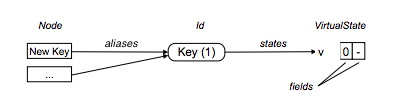
\includegraphics[width=0.9\textwidth]{DS-schema.png}
\caption{Schema of Basic Data Structures. \cite{stadler2014partial}}
\label{figure-6}
\end{figure}

Αυτά τα αντικείμενα \textit{dictionaries} λέγονται \textit{state} γιατί
διατηρούν την κατάσταση των μεταβλητών για το εκάστοτε \texttt{Block}s που
βρίσκεται τώρα ο μεταγλωττιστής. Κάθε φορά που η επεξεργασία μετακινείται στο
επόμενο \texttt{Block} τότε δημιουργείται ένα αντίγραφο του \textit{state}.
Επιπλέον λεπτομέρειες για ποιό λόγο και πως συμβαίνει αυτό στο Κεφάλαιο 4.
Λοιπόν η πληροφορία για την κατάσταση των τρέχουσων μεταβλητών βρίσκεται σε αυτή
την δομή με μορφή αντικειμένων και όπως θα δούμε όταν υπάρχει ένα τέτοιο
αντικείμενο για μια μεταβλητή (συνδεόμενο φυσικά με αυτή με aliases και ids στο
\textit{state}) τότε το αντικείμενο είναι πάντα εικονικό. Αν δεν είναι εικονικό
το \texttt{VirtualObject} διαγράφεται από το \textit{state}, σε αντίθεση με την
μέθοδο που ακολουθείται στο paper. Εκεί προτείνεται η ύπαρξη δύο είδών εικονικών
αντικειμένων – ένα για την περίπτωση εικονικότητας (\texttt{VirtualState}) και
ένα για την περίπτωση αναγκαιότητάς του (\texttt{EscapedState}). Οι διαφορές
ήταν μικρές και κρίναμε ότι δεν ήταν αναγκαίο να υπάρχει κατάσταση και
αντικείμενο πληροφοριών για ένα αντικείμενο που υπάρχει στην μνήμη έτσι και
αλλίως αυτό καθ' αυτό.

Όπως βλέπουμε στο \ref{figure-6}, το πρώτο λευκό κουτάκι είναι το ``node". Δηλαδή
μια αφαιρετική έννοια που περιλαμβάνει κυρίως ονόματα και references σε
μεταβλητές που υπήρχαν στην αρχική έκδοση του κώδικα. Αυτά ``δείχνουν" στο id, το
οποίο είναι ουσιαστικά το όνομα που έχουμε δώσει στην μεταβλητή\footnote{ή
μεταβλητές} αυτή εσωτερικά – για δική μας χρήση μέσα στο σύστημά μας. Αυτό
δείχνει φυσικά στο εικονικό αντικείμενο που είναι μοναδικό για κάθε μεταβλητή
ανεξάρτητα από το πόσα ονόματα (aliases) έχει. Στην πραγματικότητα
χρησιμοποιούμε ένα \textit{defaultdict} της Python για να δείχνουμε κατευθείαν
απο τα nodes στα αντίστοιχα εικονικά αντικείμενα. Αυτό που φαίνεται στην εικόνα
είναι το θεωρητικό μοντέλο μας.

Να πούμε επίσης ότι στο paper εξηγείται πλήρως – και υπάρχει στο μοντέλο του – ο
τρόπος για το \textit{handling} όλων αυτών των διαδικασιών με δυνατότητες
κλειδώματος (locking) για παράλληλη επεξεργασία (βλ. \textit{multithreading}).
Εμείς δεν το συμπεριλαμβάνουμε αυτό, καθώς:

\begin{enumerate}

\item Δεν είναι αναγκαίο γιατί ασχολούμαστε με μεταγλωττιστές, ο εσωτερικός
κώδικας των οποίων δεν είναι συνήθως \textit{multi-threaded}.

\item Ακόμαι και αν χρειαστεί η δυνατότητα, η Python δεν το υποστηρίζει καλά
λόγω του καθολικού κλειδώματος που έχει (Global Interpreter Lock).

\end{enumerate}

%%%%%%%%%%%%%%%%%%%%%%%%%%%%%%%%%%%%%%%%%%%%%%%%%%%%%%%%%%%%%%%%%%%%%%

\subsection{Πότε αλλάζουν τα states}

Οι περιπτώσεις που επειρεάζονται τα state αντικείμενα – σύμφωνα πάντα με την
ιδανική κατάσταση του paper\cite{standler2014partial} και την υλοποίησή τους σε
Java (η οποία είναι ένας βελτιστοποιητής στον μεταγλωττιστή της που λέγεται
\textit{Graal}) – ή αλλιώς αυτά που χρήζουν προσοχής είναι:

\begin{itemize}

\item Κόμβοι (δηλαδή \texttt{Block}s) που περιέχουν εντολές δέσμευσης μνήμης
στον σωρό (malloc). Θα δημιουργήσουν εικονικά αντικείμενα.

\item Εντολές που κάποιο από τα argument τους περιέχουν keys σε υπάρχοντα
εικονικά αντικείμενα ή aliases σε αυτα. Οι εντολές τότε πρέπει να επεξεργαστούν
και είτε να μεταβληθούν είτε να αφαιρεθούν από τον κώδικα ολοκληρωτικά.

\item \texttt{Block}s που είναι ειδικά όπως \textit{mergeblock}
\textit{Returnblock} και \textit{LoopBegin}.

\end{itemize}

%%%%%%%%%%%%%%%%%%%%%%%%%%%%%%%%%%%%%%%%%%%%%%%%%%%%%%%%%%%%%%%%%%%%%%

\subsection{Πώς αλλάζουν τα states}

Θεωρητικά, σύμφωνα πάντα με το paper, αυτές οι αλλαγές στα states είναι οι
παρακάτω (τα γράμματα στις παρακάτω περιγραφές αντιστοιχούν στις εικόνες
\ref{figure-21} έως \ref{figure-24}):

\begin{enumerate}[label=\alph*]

\item Για κάθε δέσμευση, δημιουργούνται καινούργια εικονικά αντικείμενα \\
(\texttt{VirtualObject} – VOs) και τα αντίστοιχα entries στα mapping
dictionaries.

\begin{figure}[h]
\centering
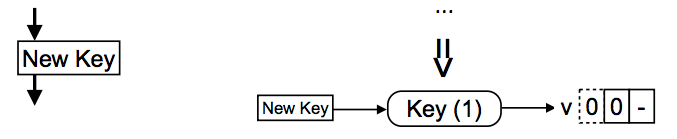
\includegraphics[width=0.5\textwidth]{virtual-alloc.png}
\caption{(ά) Actions upon allocation of a VO. \cite{stadler2014partial}}
\label{figure-21}
\end{figure}

\item Για κάθε ``ανάθεση" (εντολή \texttt{setfield}) αντικειμένου που δεν είναι
σε κάποιο dictionary (states ή aliases – στην δική μας υλοποίηση: μόνο states)
σε πεδίο εικονικού αντικειμένου μεταβάλλεται η αντίστοιχη θέση μνήμης στο
attribute του εικονικού αντικειμένου ώστε αυτό να ``ξέρει" περί της ανάθεσης. Το
γεγονός ότι το πρώτο αντικείμενο δεν ανήκε σε κάποιο dictionary μας δείχνει ότι
δεν είναι και αυτό εικονικό αντικείμενο, καθώς αν ήταν θα υπήρχε το alias του
στο dictionary. Αρα η παραπάνω περίπτωση είναι η περίπτωση ανάθεσης πραγματικού
– υπάρχοντος – αντικειμένου σε εικονικό.

\begin{figure}[h]
\centering
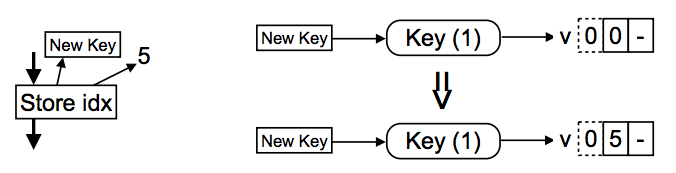
\includegraphics[width=0.5\textwidth]{virtual-ext-store.png}
\caption{(β') Actions upon simple external object storing inside a VO. \cite{stadler2014partial}}
\label{figure-22}
\end{figure}

\item Από την άλλη υπάρχει και η περίπτωση ανάθεσης εικονικού αντικειμένου σε
επίσης εικονικό αντικείμενου. Εδώ, θα αποθηκευτεί-ανατεθεί ένα
\textit{reference} του id του αντικειμένου που θα αποθηκευτεί, μέσα στο
αντικείμενο που αποθηκεύεται.

\begin{figure}[h]
\centering
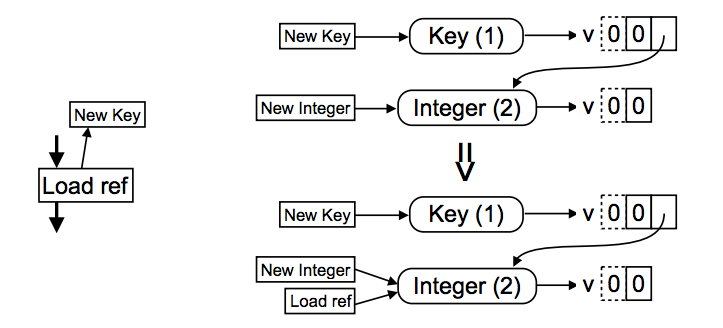
\includegraphics[width=0.5\textwidth]{virtual-virtual-load.png}
\caption{(γ') Actions upon assignment/loading of a VO inside another VO. \cite{stadler2014partial}}
\label{figure-23}
\end{figure}

\item Το παράνω φυσικά αναφέραται στην περίπτωση που θέλουμε να αποθηκέυσουμε
(store) το αντικείμενο. Στην αντίθετη, δηλαδή όταν θέλουμε να το ανακτήσουμε
μέσα από ένα άλλο που είναι επίσης εικονικό (με την εντολή \texttt{getfield}),
τότε η ανάγνωση αυτή θα οδηγήσει σε ανάθεση ενός καινούργιου alias έτσι ώστε ο
καινούργιος κώδικας, με τον οποίο θα αντικατασταθεί ο παλιός, να ξέρει που
υπάρχουν τώρα τα δεδομένα που χρειάζεται για την στιγμή που θα χρειαστεί να
γίνει το πραγματικό Load στο runtime.

\begin{figure}[h]
\centering
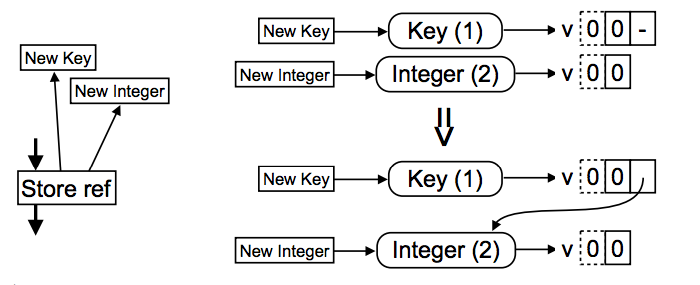
\includegraphics[width=0.5\textwidth]{virtual-virtual-store.png}
\caption{(δ') Actions upon storing a VO inside another VO. \cite{stadler2014partial}}
\label{figure-24}
\end{figure}

\end{enumerate}

Όλα αυτές οι εντολές θα αφαιρεθούν από τον κώδικα αφού, μόλις είπαμε οι
ενέργειες που λαμβάνει ο μεταγλωττιστής όταν τις συναντά αρκούν για να τις
κάνουν λειτουργικές και για τα side effects τους. Πολλές άλλες εντολές μπορούν
επίσης να αφαιρεθούν βάσει στις πληροφορίες που έχουμε στο states. Tests
ισότητας μεταξύ αντικειμένων επιστρέφουν πάντα \textit{false} αν ένα και μόνο
ένα από τα αντικείμενα που λάμβάνει το test είναι εικονικό. Εάν είναι και τα δύο
εικονικά, τότε θα παραχθεί \textit{true} αν φυσικά αναφέρονται στο ίδιο id, και
\textit{false} σε άλλη περίπτωση. (Αυτό το τσεκάρισμα, αργότερα στην υλοποίηση,
θα γίνεται κυρίως σε merge nodes όταν έχουμε αποφανθεί ότι το αντικείμενο θα
πρέπει να επανατοποθετηθεί στον κώδικα και θα θέλουμε να δοκιμάσουμε αν τα
αντικείμενα είναι ένα ή δυο.) Tests τύπων μπορούν να εκτελεστούν και σε αυτό το
σημείο (compile time). Αν κάποια εντολή που δεν είναι ειδική για αυτές τις
ενέργειες και δεν αναφέρεται εδώ απαιτεί ένα reference σε αντικείμενο το οποίο
είναι εικονικό τότε φυσικά αυτό θα πρέπει να επανατοποθετηθεί.

%%%%%%%%%%%%%%%%%%%%%%%%%%%%%%%%%%%%%%%%%%%%%%%%%%%%%%%%%%%%%%%%%%%%%%%%%%

\subsection{Ειδικές κατηγορίες: Merge}

Όταν πολλά branches της ροής θα συναντηθούν σε ένα \textit{mergenode}, πρέπει να
παράγουμε ένα state από όσα και τα branches. Αρχικά ο ``επεξεργαστής" της
συγχώνευσης θα δημιουργήσει μια \textit{τομή} από όλα τα δεδομένα των
αντικειμένων state από όλα τα branches. Αυτό σημαίνει ότι τα εικονικά
αντικείμενα που θα επιβιώσουν την συγχώνευση είναι αυτά που είναι κοινά σε όλα
τα branches της ροής και έχουν τουλάχιστον έναν κοινό alias.

Οι περιπτώσεις που μπορούν να συμβούν ανάλογα με την κατάσταση των αντικειμένων
είναι οι εξής (σχεδιαγράμματα στις εικόνες \ref{figure-41} και \ref{figure-42}):

\begin{itemize}

\item Αν το αντικείμενο έχει διαφύγει σε όλες τις προηγούμενες καταστάσεις (τις
οποίες θέλουμε να συγχωνεύσουμε) τότε φυσικά το αντικείμενο θα διαφεύγει και στο
καινούργιο state.

\item Αν κάποια από τα αντικείμενα είναι εικονικά και άλλα διαφεύγουν, τότε
πρέπει να επανατοποθετηθούν και όσα αντικείμενα είναι εικονικά στα αντίστοιχα
states τους.

\item Η πιο ειδική περίπτωση είναι όλα τα αντικείμενα να είναι εικονικά. Τότε
στο καινούργιο αντικείμενο όλες οι τιμές από όλα τα states πρέπει να
συγχωνευτούν. Για κάθε field, ο μεταγλωττιστής θα κοιτάξει και θα συγκρίνει τις
εκδόσεις από όλα τα states και:

\begin{figure}[h]
\centering
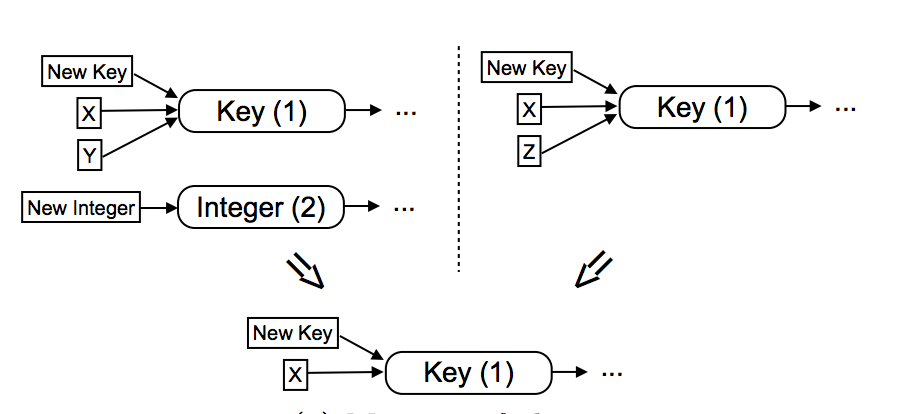
\includegraphics[width=0.5\textwidth]{merging-aliases.png}
\caption{Merging of aliases. \cite{stadler2014partial}}
\label{figure-41}
\end{figure}

\begin{figure}[h]
\centering
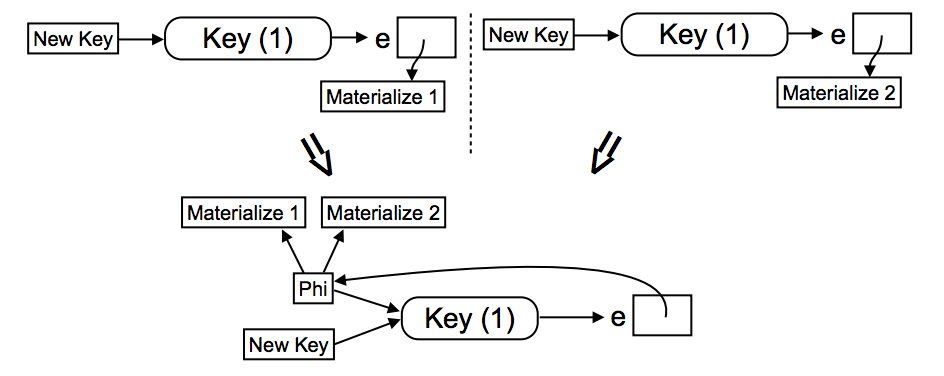
\includegraphics[width=0.5\textwidth]{merging-escaped.png}
\caption{Merging of escaped objects. \cite{stadler2014partial}}
\label{figure-42}
\end{figure}

\begin{itemize}

\item αν όλα τα πεδία είναι πανομοιότυπα και συμφωνούν, τότε το καινούργιο
αντικείμενο στο συγχωνευμένο state μπορεί επίσης να είναι εικονικό. Ο
μεταγλωττιστής θα δημιουργήσει εδώ ένα καινούργιο \texttt{VirtualObject} και θα
αντιγράψει τα fields. Τα references θα δείχνουν στα ίδια ids κτλ.

\item αν κάποιο από τα πεδία διαφέρει το αντικείμενο πρέπει να επανατοποθετηθεί,
όπως επίσης και τα αντικείμενα για τα οποία περιέχει αναφορές.

\end{itemize}
\end{itemize}

Φυσικά αυτή η διαδικασία μπορεί να οδηγήσει στην επανατοποθέτηση αντικειμένων
που σημαίνει ότι προηγούμενες υποθέσεις που έχουν γίνει για τον κώδικα δεν είναι
πλέον αληθείς άρα θα πρέπει να γίνει επεξεργασία ξανά. Οπότε επαναλαμβάνουμε το
παραπάνω μέχρι να μην υπάρχουν αλλαγές.

%%%%%%%%%%%%%%%%%%%%%%%%%%%%%%%%%%%%%%%%%%%%%%%%%%%%%%%%%%%%%%%%%%%%%%%%%%

\subsection{Ειδικές κατηγορίες: Loops}

Οι βρόγχοι (loops) είναι μια πολύ ειδική περίπτωση. Όλοι οι κόμβοι
(\texttt{Block}s) που συμμετέχουν σε έναν βρόγχο πρεπεί και θα εξεταστούν με
σεριακό τρόπο ακολουθώντας την σειρά ροής, όμως αυτό ενέχει πρόβλημα με τις
``ακμές επιστροφής" (back edges) του βρόγχου. Φυσικά η κανονική ροή εδώ μπορεί να
επισκεφτεί κόμβους παραπάνω από μια φορά – αυτό είναι και το νόημα των loops –
αλλά εμείς δεν μπορούμε να το έχουμε αυτό κατα το compile time.

Η θεωρία που ακολουθείται στο paper, έχει φυσικά το παραπάνω χαρακτηριστικό αλλά
κρίναμε ότι είναι τουλάχιστον μη αποδοτική και δεν την υλοποιήσαμε στο δικό μας
σύστημα. Συνοπτικά να πούμε ότι ξεκινάει ``μαντεύοντας" ένα state αντικείμενο (το
καλούν speculative) βάσει του κόμβου πατέρα του αρχικού κόμβου του βρόγχου και
από εκεί συνεχίζουν ακολουθώντας την ροή, σταματώντας μόνο στα back edges και
στα exits του loop. Το τελικό προϊόν είναι σωστό και η επεξεργασία συνεχίζεται
μόνο αν το αρχικο speculative state ήταν τελικά σωστό. Αν διαφέρουν, η
διαδικασία θα ξαναγίνει και το καινούργιο state θα χρησιμοποιηθεί ως speculative
state αυτή την φορά.

%%%%%%%%%%%%%%%%%%%%%%%%%%%%%%%%%%%%%%%%%%%%%%%%%%%%%%%%%%%%%%%%%%%%%%%%%%

\subsection{Πυροδότηση \& σύνδεση με άλλους βελτιστοποιητές}

Στην θέση της μεταβλητής ή αντικειμένου που αφαιρέθηκε φυσικά θα πρέπει να
υπάρξει κάτι το οποίο ``διατηρεί" την λογική του προγράμματος ως έχει. Αυτό
μπορεί να συμβεί με διάφορους τρόπους. Συνήθως επιτυγχάνεται με αντικατάσταση
βαθμωτών στην θέση της μεταβλητής. Δηλαδή το σημείο στο οποίο ``ζητούνταν"
κάποιου είδους πληροφορία τοποθετείται ένας βαθμωτός, δηλαδή μια απλή ``φθηνή"
μεταβλητή, που απλά υπάρχει στην στοίβα (\textit{function stack}) της συνάρτησης
και όχι στον σωρό (\textit{heap}). Σε αυτόν τον βαθμωτό ο μεταγλωττιστής
τοποθετεί την απαραίτητη πληροφορία που χρειάζεται το πρόγραμμα εκείνη την
στιγμή και κανονικά θα την εξήγαγε από το αντικείμενο που αφαιρέσαμε. Φυσικά την
πληροφορία αυτή ο μεταγλωττιστής την εξάγει επίσης από το αντικείμενο αλλά κατά
την ανάλυσή μας (στο \textit{compile-time}) και όχι στο \textit{runtime}. Ο
μεταγλωττιστής αποθηκεύει προσωρινά τις πληροφορίες που χρειάζεται για τυχόν
υπολογισμούς με τα αντικείμενα (για χρήση στο επόμενο σημείο που θα απαιτηθεί
βαθμωτός) στα εικονικά αντικείμενα που αναφέρουμε παραπάνω. Αν το αντικείμενο
πρέπει να επανατοποθετηθεί όλοι αυτοί οι βαθμωτοί θα αφαιρεθούν και οι ενέργειες
θα αναιρεθούν. Τέλος να πούμε ότι φυσικά πολλές από αυτές τις πράξεις θα
μεταφερθούν (\textit{carried on}) μέσω των εικονικών αντικειμένων και των
``προσωρινών" πράξεων και τα αποτελέσματά τους απλά θα τοποθετηθούν εκεί που
χρειάζονται ``πραγματικά" – δηλαδή έξω από το scope της συνάρτησης που αναλύουμε.
Μπορεί κανείς να πει ότι αυτό είναι ένα είδος \textit{constant folding}.

Όλοι οι σύγχρονοι μεταγλωττιστές – συμπεριλαμβανομένου του PyPy – δουλεύουν με
κάποιου είδους εικονική μηχανή που αναλαμβάνει να τρέξει τον κώδικα και αυτές οι
μηχανές, εκτός απο πολλά πλεονεκτήματα ασφαλείας και ευκολίας προγραμματισμού,
έχουν φυσικά πολλούς τρόπυς βελτιστοποίησης του κώδικα, όπως έχουμε πει. Σε αυτά
περιλαμβάνεται και \textit{alias analysis} που εντοπίζει τα επιπλέον ονόματα των
μεταβλητών και σίγουρα μειώνει τον φόρτο εργασίας στην μνήμη. Επίσης
συμπεριλαμβάνεται πάντα ένας inliner (βλ. παραπάνω παράδειγμα). Η βελτιστοποίηση
με την μέθοδο μερικής διαφυγής λοιπόν είναι πολύ πιο αποδοτική από αυτά μόνη της
αλλά σίγουρα ακόμα περισσότερο όταν συνδυάζεται με επιπλέον βελτιστοποιήσεις και
τροποποιητές του κώδικα όπως το inlining.

Το \textit{inling} είναι η μεταφορά κομματιών κώδικα σε άλλα σημεία έτσι ώστε να
αποφευχθεί κάποια κλήση συνάρτησης. Ο μεταγλωττιστής φυσικά προβαίνει σε αυτό
όταν αποφανθεί ότι η κλήση αυτή καθ' αυτή – δηλαδή η δημιουργεία stack και ότι
άλλο περιλαμβάνει αυτό – είναι ακριβή και δεν αξίζει. Οπότε αντί για κλήση σε
συνάρτηση θα μεταφέρει τον κώδικα της συνάρτησης στο σημείο που βρίσκεται η ροή
την εκάστοτε στιγμή. Φυσικά πολλές φορές ο μεταγλωττιστής δεν θα το κάνει –
υπάρχει λόγος που πολλές φορές ο προγραμματιστής αποφασίζει να χρησιμοποιήσει
συναρτήσεις\footnote{εκτός από την ευκολότερη διαχείρηση του κώδικα} όταν π.χ. η
κλήση θα συμβεί πολλές φορές. Εαν προβούμε σε inlining σε αυτή την περίπτωση το
μέγεθος του κώδικα θα αυξηθεί δραματικά. Είναι προφανές ότι αυτού του είδους η
ενέργεια βοηθά το δικό μας έργο σε τεράστιο βαθμό. Οι μεταβλητές που
αποφασίζουμε ότι μπορούν να αφαιρεθούν είναι πολύ περισσότερες μετά το πέρασμα
του inliner, καθώς οποιαδήποτε μεταβλητή μπορεί να μεταφερθεί στην συνάρτηση
έχει μεταφερθεί. Ο inliner υλοποιείται στο αρχείο \texttt{inliner.py}.

Για επιπλέον πρακτικές λεπτομέρειες για το πως υλοποιήσαμε την παραπάνω θεωρία
και φυσικά ότι προβλήματα πραγματικού περιβάλλοντος συναντήσαμε κατά το
εγχείρημα αυτό βλ. επόμενο κεφάλαιο.

%------------------------------------------------------------------------------

\section{Παράδειγμα}

Εδώ παραθέσουμε ένα εκτενές παράδειγμα, αυτή τη φορά φυσικά για τις διαφορές και
λεπτομέρειες της μερικής ανάλυσης με περισσότερη \textit{real-world} λεπτομέρεια
από το αντίστοιχο της απλής ανάλυσης, ακολουθώντας φυσικά το παράδειγμα του
paper\cite{stadler2014partial} εξιδανικευμένο για την Python. Αυτή την φορά ο
αρχικός κώδικας είναι μετά το inlining για να αναδείξουμε καλύτερα τα
αποτελέσματα της ανάλυσης διαφυγής.

\begin{lstlisting}[language=Python]
...
def getValue(idx, ref):
    key = Key()
    key.idx = idx
    key.ref = ref
    tmp1 = cacheKey # getting from a global
    tmp2 = (key.idx == tmp1.idx && key.ref == tmp1.ref)
    if tmp2:
        return cacheValue
    else:
        cacheKey = key # assigning to a global
        cacheValue = createValue(...)
        return cacheValue
...
\end{lstlisting}

Ξανά δεν δίνουμε τις καθολικές (global) μεταβλητές (βλ. γραμμή 5) και πολλές
λεπτομέρειες που θα επιβάρυναν τον κώδικα χωρίς να προσφέρουν επιπλέον
πληροφορία. Αναδεικνύουμε παρακάτω πως θα ήταν σε κώδικα Python η
βελτιστοποιημένη έκδοση του παραπάνω κώδικα. Επαναλαμβάνουμε ότι αυτή η
λειτουργία γίνεται σε γραφήματα ροής.

\begin{lstlisting}[language=Python]
...
def getValue(idx, ref):
    tmp = cacheKey
    if (key.idx == tmp.idx && key.ref == tmp.ref):
        return cacheValue
    else:
        key = Key()
        key.idx = idx
        key.ref = ref
        cacheKey = key
        cacheValue = createValue(...)
        return cacheValue
...
\end{lstlisting}

Βλέπουμε τον τρόπο που ο βελτιστοποιητής άλλαξε τον κώδικάς μας.

\begin{itemize}

\item Στην γραμμή 3 η δέσμευση (η δημιουργία ουσιαστικά του αντικειμένου) έχει
αφαιρεθεί. Δημιουργείται εικονικό αντικείμενο.\footnote{Για περισσότερες
λεπτομέρειες για τα εικονικά αντικείμενα βλ. προηγούμενο κεφάλαιο}

\item Οι αναθέσεις στις γραμμές 4 και 5 έχουν επίσης αφαιρεθεί. Γίνεται
``ανάκλαση" των αποτελεσμάτων τους και των side-effect τους στα εικονικά
αντικείμενα.

\item Οι απόπειρες πρόσβασης σε περιοχές δεσμευμένης μνήμης στην γραμμή 7 έχουν
αντικατασταθεί με απλές προσβάσεις σε τοπικές περιοχές.

\item Στην περίπτωση του \texttt{if} στην γραμμή 8, δημιουργείται ένα επιπλέον
αντίγραφο της δομής δεδομένων που διαχειρίζεται τα εικονικά αντικείμενα
(\textit{state} – βλ. παρακάτω).

\item Στην γραμμή 9 το αντικείμενο είναι ακόμα εικονικό. Λόγω της εντολής
\texttt{return} η διαδικασία ανάλυσης αυτού του branch (του if) τερματίζει εδώ.

\item Η ανάλυση για το δεύτερο branch όμως συνεχίζεται στο \textit{else case}
εδώ. Στην στιγμή της γραμμή 11 το αντικείμενο είναι ακόμα εικονικό όμως λόγω της
ανάθεσης σε καθολική μεταβλητή θα ``διαφύγει". Για να μπορεί να γίνει αυτό όμως,
το αντικείμενο θα πρέπει να υπάρχει αυτό καθ' αυτό, οπότε θα πρέπει να
τοποθετηθεί στον κώδικα η δέσμευση της μνήμης, η αρχικοποίησή της, η ανάθεση των
field σύμφωνα με το εικονικό αντικείμενο (και ότι άλλο υπεισέρχεται στην
δημιουργία ενός αντικειμένου). Ονομάζουμε αυτή την διαδικασία
\textit{materialization} (βλ. επόμενο κεφάλαιο).

\item Οι γραμμές 12 και 13 δεν επηρεάζουν πλέον την κατάσταση του κώδικα – αφού
έχουμε ήδη αποφανθεί ότι το αντικείμενο πρέπει να υπάρχει.

\end{itemize}

Γενικά, όπως βλέπουμε, η δέσμευση και όλες οι ακριβές ενέργειες έχουν
τοποθετηθεί ακριβώς εκεί που απαιτούνται και όχι οπουδήποτε αλλού – δηλαδή στο
\textit{else case} του \textit{if branch}. Αυτό προφανώς δεν οδηγεί σε μικρότερο
αριθμό εντολών \texttt{malloc} (ούτε άλλων ακριβών εντολών) αλλά μειώνει τον
δυναμικό αριθμό των δεσμεύσεων μνήμης αφού αυτοί θα συμβούν πιο σπάνια δεδομένου
ότι βρίσκονται σε ένα από τα \textit{cases} και όχι στην κυρίως ροή του κώδικα.
Με άλλα λόγια μειώνουν το μέσο κόστος της συνάρτησης, βασιζόμενοι στην μικρότερη
συχνότητα με την οποία τρέχουν τα \textit{branches}. Όπως θα δούμε στο κεφάλαιο
των μετρήσεων (Κεφ. 5.) αυτό συμβαίνει συχνά.

%------------------------------------------------------------------------------

\chapter{Υλοποίηση}
\label{chapter4}

\section{Γενικά}

Σε αυτό το κεφάλαιο θα αναλύσουμε τις λεπτομέρειες περί της υλοποίησης και τις
δυσκολίες που προέκυψαν σε αυτή. Η βάση μας είναι ένα προηγούμενο paper των
Standler, W{\"u}rthinger et al\cite{stadler2014partial} που μελετά, περιγράφει
και υλοποιεί την μέθοδο για την γλώσσα Java. Ακολουθήσαμε σε γενικές γραμμές –
και ειδικότερα στην αρχή – τις περιγραφές που δίνουν για την υλοποίηση και
δομήσαμε την υλοποίησή μας όμοιως. Βέβαια όσο προχωρούσαμε τόσο αποκλίναμε από
αυτή την περίπτωση, καθώς εμείς είχαμε να κάνουμε με μια δυναμική γλώσσα σε
αντίθεση με την στατική Java. Επιπλέον πολλές λεπτομέρειες έλειπαν από την
εργασία.

Ο κυρίως κώδικας (δηλαδή το αρχείο \texttt{partial\_escape.py}) δίνεται στο
παράρτημα Α'. Οι γραμμές κώδικα που εμφανίζονται στο παρακάτω κείμενο
αναφέρονται σε αυτόν.

Όπως έχουμε ήδη αναφέρει ο κώδικας του project του PyPy χωρίζεται σε
subsystems, και modules. Το module που υλοποιούμε υπόκειται στο σύστημα
RPython, στο subsystem του translator, στην ομάδα των backend
βελτιστοποιήσεων. Βρίσκεται επομένως στο ακόλουθο μονοπάτι:
\path{pypy/rpython/translator/backendopt/partial_escape.py}. Ο κώδικας
βρίσκεται σε ένα fork\cite{fork} του επίσημου \textit{repository} του
PyPy\cite{repo} στη σελίδα bitbucket\footnote{\url{http://bitbucket.com}}. Η
υλοποίηση έγινε με την βοήθεια του εργαλείου διαχείρησης εκδόσεων κώδικα (SCM)
mercurial\cite{mercurial} το οποίο χρησιμοποιείται και εσωτερικά από το
project. Φυσικά γίνονται προσπάθειες προκειμένου το module μας να
συμπεριληφθεί στο επίσημο repo του PyPy.


\subsection*{Test-driven development}

Στην υλοποίηση χρησιμοποιήθηκε η μέθοδος ανάπτυξης λογισμικού βασισμένη σε
tests (\textit{test-driven development}\cite{tdd}). Είναι μια σχετικά
καινούργια μέθοδος ανάπτυξης που χρησιμοποιεί test κώδικα για να ελέγξει την
ορθότητα του κανονικού κώδικα των προγραμμάτων. Η μέθοδος αναπτύχθηκε φυσικά
λόγω της μεγάλης πολυπλοκότητας που έχουν τα διάφορα προγράμματα και συστήματα
την σήμερον ημέρα. Ο προγραμματιστής αφού κατανοήσει περίπου πως πρέπει να
δομήσει το πρόγραμμα του ξεκινά με την συγγραφή του test κώδικα. Αρχικά για
τις απλές (και ίσως τετριμένες) περιπτώσεις και σταδιακά αυξάνει την
πολυπλοκότητα των tests και φυσικά του κώδικα αντιστοίχως. Αφού γράψει ένα ή
περισσότερα tests, συγγράφει το πρόγραμμά του προσπαθώντας να κάνει τα tests
να "τρέξουν" επιτυχώς. Η διαδικασία συνεχίζεται φυσικά μέχρι να ολοκληρωθεί η
διαδικασία ανάπτυξής ή να φτάσει ο προγραμματιστής στην επιθυμητή
πολυπλοκότητα. Με αυτόν τον τρόπο – αν προφανώς όλα τα tests είναι επιτυχή – ο
προγραμματιστής είναι σίγουρος ότι οι καινούργιες αλλαγες που επέφερε στο
project δεν επηρέασαν την ορθότητα του προγράμματος σε κάποιο προηγούμενο
στάδιο.

Το PyPy χρησιμοποιεί αυτή την μέθοδο, οπότε και η υλοποίησή μας την ακολουθεί.
Ο test κώδικας του module που υλοποιήθηκε βρίσκεται στο ακόλουθο μονοπάτι:
\path{pypy/rpython/translator/backendopt/test/test_partial_escape.py}. Δεν
συμπεριλαμβάνεται στην εργασία αυτή για λόγους λακωνικότητας.

%------------------------------------------------------------------------------

\section{Δομή του κώδικα}

\subsection{Βασική Συνάρτηση}

Ο κώδικας είναι σε ένα αρχείο. Χωρίζεται φυσικά σε συναρτήσεις. Η κυρίως
συνάρτηση είναι η \texttt{partial\_escape()}. Αυτή αποτελεί το κυρίως module που
θα τρέξει για κάθε γράφημα με σκοπό την βελτιστοποίηση. Το σύστημα θα καλεί την
συνάρτηση αυτή δίνοντας της ένα γράφημα την φορά σε ένα loop. Τα διαθέσιμα
γραφήματα θα είναι όλες οι συναρτήσεις του μεταγλωττιστή. Το γράφημα
μεταβάλλεται \textit{in-place} και το return value είναι ένας μετρητής των
\texttt{getfield} εντολών που αφαιρέθηκαν. Πρακτικά η μείωση των εντολών
\texttt{getfield} στο γράφημα είναι ο κύριος στόχος της συνάρτησης καθώς το
module μας θα τρέξει μετά το ήδη υπάρχον module για ανάλυση διαφυγής (non-
partial escape analysis) στο PyPy. Παρόλα αυτά δεν είναι μόνο αυτή η αλλαγή που
επιφέρεται από το module. Σίγουρα αφαιρούνται πολλές εντολές \texttt{malloc} –
οι οποίες είναι εξαιρετικά ακριβές. Επιπλέον πολλές ακριβές εντολές
μετακινούνται σε κάποιο μονοπάτι της ροής εκτέλεσης το οποίο εκτελείται σπάνια ή
λιγότερες φορές, οπότε εν δυνάμει είναι σαν να αφαιρούνται.


\subsection{worklist}

Με τον όρο \textit{Worklist} καλούμε την δομή δεδομένων που χρησιμοποιούμε για
να μας βοηθά στην επιλογή του επόμενου \texttt{Block} προς επεξεργασία.
Επιλέξαμε ένα deque\cite{deque} (από τα εσωτερικά structures της Python από το
module \texttt{collections}). Γενικά, στον κώδικα, χρησιμοποιούμε πολύ συχνά
constructions της Python προς διευκόλυνσή μας. Ένα deque ή dequeue
(\textit{double ended queue}) είναι μια ουρά (queue) που έχει δυνατότητα
εισαγωγής και εξαγωγής και από τις δύο άκρες. Η επιλογή του επόμενου
\texttt{Block} εξαρτάται από πολλούς παράγοντες – η μεγαλύτερη πολυπλοκότητα
απαντάται στην περίπτωση των loops, καθώς κάθε \texttt{Block} πρέπει να
επεξεργαστεί προφανώς μόνο μια φορά και στην σωστή σειρά. Μια τέτοια δομή
δεδομένων ήταν η ιδανική για τον σκοπό μας. Η επεξεργασία του \textit{worklist}
γίνεται στο τέλος κάθε iteration επεξεργασίας κάποιου \texttt{Block} (στις
γραμμές $371-381$ του κώδικα.)

\subsection{Αφαίρεση μεταβλητών και αντικατάσταση με βαθμωτούς}

Όταν ο μεταγλωττιστής εντοπίσει μια καινούργια μεταβλητή τότε την αφαιρεί από
τον κώδικα, δημιουργεί ένα εικονικό αντικείμενο (βλ. παρακάτω) και την
"παρακολουθεί". Δηλαδή ανιχνεύει τις ενέργειες που γίνονται με αυτή, καταγράφει
τις εντολές που τρέχουν και τις αντικαθιστά αναλόγως, έτσι ώστε η λογική, η
εκτέλεση, και η ορθότητα του προγράμματος να παραμένει ίδια παρόλο που
αφαιρέσαμε μια ολόκληρη μεταβλητή. Για παράδειγμα το παρακάτω κομμάτι κώδικα:

\begin{lstlisting}[language=Python, deletendkeywords={id}]
k = Key()
k.id = 1
\end{lstlisting}

θα μεταφραστεί σε:

\begin{lstlisting}[language=Python, deletendkeywords={id}, keywords={malloc}]
k1 = malloc(...)
setfield(k1, id, 1)
\end{lstlisting}

Εκτός από την αφαίρεση της εντολής \texttt{malloc} εδώ, θα αφαιρεθεί επίσης και
η εντολή \texttt{setfield}, καθώς έχει να κάνει με το αντικείμενο που
αφαιρείται. Εκτός από την αφαίρεση, η κάθε εντολή έχει φυσικά και συνέπειες για
τα εικονικά αντικείμενα. Για παράδειγμα η \texttt{setfield} προκαλεί το
\textit{set} σε ένα από τα fields του εικονικού αντικειμένου σύμφωνα με τα
ορίσματά της. Στο παραπάνω παράδειγμα θα δημιουργηθεί ένα field "id" στο
εικονικό αντικείμενο. Επίσης (εκτός από την \texttt{malloc} και την
\texttt{setfield}) υπάρχουν και άλλες εντολές που είτε μεταβάλλονται είτε
μεταβάλλουν τα εικονικά αντικείμενα. Η σημαντικότερη από αυτές είναι η εντολή
\texttt{getfield}. Αυτή η εντολή είναι το σημείο που θα γίνει η πραγματική
αντικατάσταση βαθμωτού, καθώς εκεί είναι απαραίτητη η τιμή. Το \texttt{getfield}
κάνει το access σε κάποιο field μιας μεταβλητής. Εάν εμείς αφαιρέσουμε την
μεταβλητή θα πρέπει να αντικαταστήσουμε την τιμή εδώ με κάποιον αντίστοιχο
βαθμωτό ή με κάποιον υπολογισμό, σύμφωνα πάντα με τα συμφραζόμενα. Η
"πιστοποίηση" για το αν οι εντολές επηρεάζουν τα εικονικά αντικείμενα γίνεται
πολύ απλά με έναν έλεγχο για το αν το αντικείμενο υπάρχει μέσα στο
\textit{state}. Αν δεν υπάρχει τότε η εντολή έχει να κάνει με κάποιο αντικείμενο
που δεν μπορούμε να πειράξουμε είτε με κάποιο που έχει ήδη επανατοποθετηθεί (βλ.
επόμενη παράγραφο).

\subsection{materialization}

Με τον όρο \textit{materialization} καλούμε την "επανατοποθέτηση" του
αντικειμένου στον κώδικα. Αυτό περιλαμβάνει την επανατοποθέτηση των εντολών για
την δέσμευση της μνήμης και οποιασδήποτε αρχικοποίησης ή τυχών casting ή
aliasing πρέπει να εφαρμοστεί στο αντικείμενο, καθώς και την "ακύρωση"
οποιονδήποτε άλλων ενεργειών έχουμε ήδη εκτελέσει. Οι κυρίως λόγοι που μπορεί να
προκαλέσουν κάποιο αντικείμενο να κάνει materialization είναι η επιστροφή του ως
return value ή το globaliazation του, δηλαδή η αλλαγή scope του (η ανάθεσή του,
με άλλα λόγια, σε κάποια global μεταβλητή). Οι ενέργειες που πρέπει να γίνουν
φυσικά διαφέρουν ανάλογα με το αντικείμενο και ανάλογα με το πόσες εντολές (π.χ.
\texttt{setfield}) έχουν εκτελεστεί σε αυτό. Οι εντολές για την αρχικοποίησή του
(\texttt{malloc} και \texttt{cast}) θα τοποθετηθούν είτε στο προηγούμενο Block
είτε στο τρέχον. Στο τρέχον θα τοποθετηθούν αν ο μεταγλωττιστής ανακαλύψει την
ανάγκη για materialization πάνω στην κανονική επεξεργασία των εντολών ενώ στο
προηγούμενο αν την ανακαλύψει οπουδήποτε αλλού (π.χ. κατά την επεξεργασία των
link arguments).

Η πιο περίπλοκη περίπτωση είναι αυτή που το αντικείμενο περιέχει ένα reference
σε άλλο εικονικό αντικείμενο. Αν ένα εικονικό αντικείμενο πρέπει να υλοποιηθεί
ξανά (materialization) τότε πρέπει να συμβεί το ίδιο και για όλα τα εικονικά που
περιέχει. Αυτό το διαχειριζόμαστε με recursion στην συνάρτηση του
materialization, οπότε ακολουθούνται οι ίδιες ενέργειες.

Υπάρχει επίσης μια bypass δυαδική μεταβλητή η οποία μπορεί να εξαναγκάσει το
materialization (\texttt{must\_be\_materialized}).


\subsection{aliasing}

Η Python είναι δυναμική οπότε τα εσωτερικά castings των μεταβλητών και τα
διαφορετικά ονόματά τους (\textit{aliases}) βρίθουν. Το σύστημά μας έπρεπε να
διαχειρίζεται τα castings και να ακολουθεί το σύστημα με τα aliasings που
περιγράφεται από το paper έτσι ώστε να καλύψει τις περιπτώσεις όλων των
ονομάτων για τις ίδιες μεταβλητές – Η Python πολλές φορές χρησιμοποιεί
διαφορετικά ονόματα για την ίδια μεταβλητή προκειμένου να χρησιμοποιήσει
λιγότερη μνήμη. Το paper κηρύττει την χρήση ενός δεύτερου dictionary που θα
"δείχνει" στο \textit{id} που με την σειρά του θα "δείχνει" στο εικονικό
αντικείμενο. Εμείς – αφού έχουμε στην διάθεσή μας τις κατασκευές και ευκολίες
που προσφέρει η Python – χρησιμοποιούμε επιπλέον keys (στο ίδιο dictionary)
που απλά "δείχνουν" στο ίδιο εικονικό αντικείμενο. Με αυτόν τον τρόπο
διατηρούμε κάθε όνομα που υπάρχει για την μεταβλητή και μπορούμε να
"ανιχνεύουμε" για αυτά τον κώδικα κατά την μεταγλώττιση. Εκτός από αυτό,
διατηρούμε και ένα \textit{set} από τα ίδια κλειδιά/ονόματα μέσα σε κάθε
εικονικό αντικείμενο έτσι ώστε να ξέρουμε εύκολα τα κλειδιά όταν πρέπει να
επανατοποθετήσουμε το αντικείμενο στον κώδικα (βλ. materialization), αφού
προφανώς πρέπει να "υπακούει" και πάλι σε όλα τα ονόματα που είχε. Το
\textit{set} αυτό αρχικοποιείται, φυσικά, στην \texttt{\_\_init\_\_()}
συνάρτηση του \texttt{VirtualObject}.

\subsection{Άλλες συναρτήσεις και κλάσεις}

\subsubsection{VirtualObject}

Η κυρίως κλάση του module. Αντιπροσωπεύει ένα εικονικό αντικείμενο και περιέχει
ότι χρειάζεται. Είναι σχετικά απλή καθώς οι περισσότερες διαδικασίες διαχείρησης
λαμβάνουν χώρα στις συναρτήσεις. Περιέχει μόνο μια μέθοδο λ.χ. η οποία είναι η
\texttt{indencical\_malloc\_args()} και αυτό που κάνει είναι απλά να ελέγχει αν το
εκάστοτε στιγμιότυπο στο οποίο τρέχει (\textit{self}) και ένα όρισμά της, έχουν
ίδια ορίσματα στην εντολή δέσμευσης μνήμης. Η εντολή δέσμευσης μνήμης για το
κάθε αντικείμενο αποθηκεύεται μέσα στο αντίστοιχο εικονικό αντικείμενο πριν το
πρώτο αφαιρεθεί από τον κώδικα. Έκτος από αυτό, κάθε τέτοιο εικονικό αντικείμενο
αποθηκεύει ένα dictionary με όλα τα πεδία (\textit{fields}) – που μπορεί να
περιείχε το αρχικό αντικείμενο, τον τύπο του cast για το malloc του
αντικειμένου και ένα σετ με όλα τα aliases (βλ. [που?]) για το αντικείμενο.

\subsubsection{get\_current\_state()}

Απλή, βοηθητική συνάρτηση η οποία δέχεται ως όρισμα μια λίστα η οποία περιέχει
dual tuples - ζευγάρια δηλαδή, από \texttt{Link}s και \textit{states}. Αποτελεί
μια wrapper συνάρτηση που κάνει μικρότερης σημασίας τετριμμένες εργασίες. Στις
περισσότερες φορές το μέγεθος της λίστας είναι 1 (σειριακή περίπτωση) και
επιστρέφεται αμέσως το \textit{state}. Σε άλλες καλείται η συνάρτηση
\texttt{merge()} Δέχεται επίσης την bypass μεταβλητή
\texttt{must\_be\_materialized} και την περνάει στις επόμενες συναρτήσεις όπου
χρειάζεται.

\subsubsection{can\_remove()}

Απλή, βοηθητική συνάρτηση η οποία χρησιμοποιείται για να κρίνει εάν το δοθέν
αντικείμενο μπορεί να αφαιρεθεί με ασφάλεια. Οι έλεγχοι που κάνει είναι
δευτερεύοντες, καθώς το αν το αντικείμενο μπορεί να αφαιρεθεί ή όχι είναι το όλο
νόημα της βελτιστοιποίησης αυτής. Περιλαμβάνουν τελικούς ελέγχους για το αν το
αντικείμενο λ.χ. έχει destructors\footnote{Εξαιρέσαμε τα αντικείμενα με
destructors από την ανάλυση γιατί αυξάνονταν η πολυπλοκότητα χωρίς πολύ κέρδος
στον χρόνο και στην μνήμη.} ή αν είναι υπόκειται σε garbage collection.

\subsubsection{remove\_virtual\_inputargs()}

Επίσης απλή, βοηθητική συνάρτηση που εκτελεί ένα είδους "syncing" μεταξύ δύο
λιστών. Κάνει ένα iteration στα αντικείμενα του \textit{state} και διαγράφει την
αντίστοιχη μεταβλητή στα \texttt{inputargs} των \texttt{Block}s και των
\texttt{Link}s για οποιαδήποτε από αυτά υπάρχει. Αυτές είναι πλέον άχρηστες
καθώς χρησιμοποιούνταν πριν για να αναφερθούν σε αυτό, ενώ τώρα το αντικείμενο
δεν υπάρχει αφού είναι εικονικό.

\subsubsection{materialize\_object()}

Μια από τις τρεις δευτέροντες βασικές συναρτήσεις του module. Αναλαμβάνει το
materialization του αντικειμένου για το οποίο θα καλεστεί. Δέχεται ως όρισμα το
"κλειδί" του αντικειμένου αυτού στο \textit{state}, το ίδιο το \textit{state}
και την λίστα με τις εντολές (operations). Στην λίστα αυτή θα προστεθούν οι
εντολές που απαιτούνται. Αυτή μεταβάλλεται \textit{in- place} και
χρησιμοποιείται από την καλούσα συνάρτηση για να αντικαταστήσει τις εντολές του
\texttt{Block}.

Λειτουργεί επίσης ως "κριτής" για την συνάρτηση που την κάλεσε, καθώς
επιστρέφει \texttt{True} ή \texttt{False} ανάλογα με το αν η λειτουργία της ήταν
επιτυχής.

\subsubsection{merge()}

Αυτή η συνάρτηση αναλαμβάνει να συγχωνεύσει δύο ή περισσότερα \textit{states} σε
ένα ανάλογα με τα εικονικά αντικείμενα και φυσικά το context από τα
\texttt{Block}s και τα \texttt{Link}s. Δέχεται (και αυτή) την λίστα με τα
δυαδικά tuples από \textit{states} και \texttt{Link}s. Καλείται μόνο από την
συνάρτηση \texttt{get\_current\_state()} εάν χρειάζεται, δηλαδή σε περιπτώσεις
if και loop. Η μεταβλητή \texttt{must\_be\_materialized} κυρίως επηρεάζει την
λειτουργία αυτής της συνάρτησης.

Για περισσότερες λεπτομέρειες βλ. παράγραφος Merge.

\subsubsection{copy\_state()}

Η τελευταία από τις τρεις δευτέροντες βασικές συναρτήσεις του module. Η
λειτουργία της είναι η αντιγραφή του \textit{state} για το επόμενο
\texttt{Block}. Φυσικά θα εκτελέσει και οποιεσδήποτε άλλες ενέργειες
απαιτούνται. Δέχεται προφανώς μια αντικείμενο \textit{state}, και επιπλέον ένα
\texttt{Link}\footnote{κυρίως απαιτούνται τα arguments και το target
\texttt{Block}}, και την ειδική μεταβλητή \texttt{must\_be\_materialized}.
Επιστρέφει ένα καινούργιο αντικείμενο \textit{state} φτιαγμένο για το καινούργιο
\texttt{Block}. Μπορεί με την πρώτη ματιά η υλοποίησή αυτής της συνάρτησης να
φαίνεται τετριμμένη, όμως έκρυβε δυσκολίες. Κατ' αρχάς η αντιγραφή ενός τέτοιο
dictionary είναι αυτή καθ' αυτή δύσκολη καθώς τα εικονικά αντικείμενα θα έχουν
διαφορετικά ονόματα στο επόμενο \texttt{Block} – δηλαδή άλλες μεταβλητές που θα
δείχνουν σε αυτά, οπότε πρέπει να αντιστοιχηθούν σωστά. Αυτό συμβαίνει γιατί το
σύστημα των γραφημάτων στο PyPy είναι προγραμματισμένο να χρησιμοποιεί
καινούργιες μεταβλητές σε κάθε καινούργιο \texttt{Block} για λόγους ανεξαρτησίας
των \texttt{Block}s. Η αντιστοιχία γίνεται ένα προς ένα μεταξύ των λιστών ενός
\texttt{Block} και ενός \texttt{Link}. Λ.χ. το πρώτο μέλος της λίστας από τα
arguments του \texttt{Block} θα μπει στην μεταβλητή που υπάρχει επίσης στο πρώτο
μέλος της λίστας του \texttt{Link}. Φυσικά αυτές οι λίστες θα πρέπει επίσης να
είναι "συγχρονισμένες" με το ποια αντικείμενα είναι εικονικά και αυτές οι
αλλαγές λαμβάνουν χώρα εδώ. Όταν ένα αντικείμενο υπάρχει στο \textit{state} τότε
οποιαδήποτε μεταβλητή αναφέρεται σε αυτό στα arguments θα πρέπει να σβηστεί. Ο
κύριως σχεδιασμός της έγινε κατά την φάση υλοποίησης Split (βλ. παρακάτω).

%-----------------------------------------------------------------------------

\section{Γραφήματα}

Η όλη διαδικασία ουσιαστικά αλλάζει το γράφημα που δέχεται ως είσοδο. Αν η
συνάρτησή μας δεχτεί ως όρισμα το γράφημα \ref{figure-2} τότε θα επιστρέψει το
βελτιστοποιημένο ως προς τα \texttt{mallocs} γράφημα που φαίνεται παρακάτω στο
\ref{figure-3}.

\begin{figure}[h]
\centering
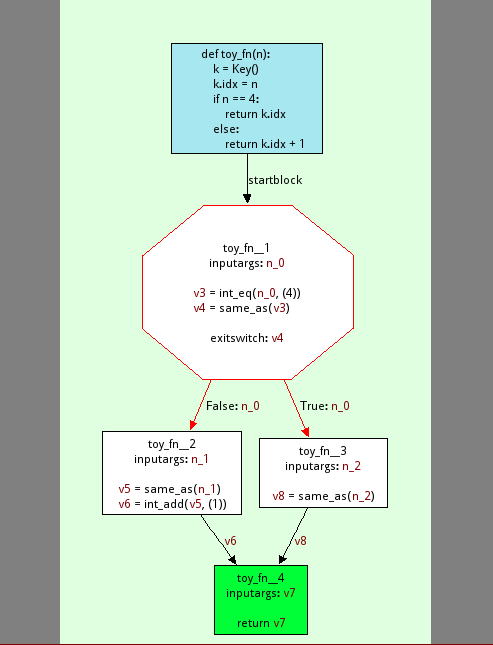
\includegraphics[width=0.6\textwidth]{simple-func-after.png}
\caption{Simple function flow diagram after the optimization took place.}
\label{figure-3}
\end{figure}

\subsection{Πως μεταβάλλουμε τα γραφήματα}

Τα γραφήματα εσωτερικά ορίζονται στο \path{pypy/rpython/flowspace/model.py} και
σχεδιάζονται από το εξωτερικό module pygame. Μπορούμε μέσω μιας μεταβλητής graph
να βρούμε σειριακά όλα τα \texttt{Block} και \texttt{Link}s και μετά στο μέλος
\texttt{operations} του \texttt{Block} υπάρχει η λίστα με τις εντολές.
Μεταβάλλοντάς την μπορούμε να μεταβάλουμε το \texttt{Block} οπότε και το
γράφημα. Φυσικά τα παραπάνω είναι υπεραπλουστευμένα, αλλά δίνουν μια καλή
εικόνα. Για σωστή διαχείριση απαιτούνται επιπλέον πληροφορίες αλλά το σύστημα
του framework του PyPy παρέχει ότι μπορεί να χρειαστεί ο προγραμματιστής. Το
\texttt{Block} λ.χ. περιέχει επίσης λίστες με τα \textit{exits} του, λίστα με τα
ορίσματα που δέχεται\footnote{Το κάθε \texttt{Block} δέχεται – όπως και οι
συναρτήσεις – ορίσματα και "επιστρέφει" μεταβλητές στα επόμενα μέσω των
\texttt{Link}s}, βοηθητικές συναρτήσεις (π.χ. \texttt{is\_final\_block()}), τη
μεταβλητή exitswitch που χρησιμοποιείται για τα branches (ifs), και τέλος
πληροφορίες για την διαχείριση του από το σύστημα του μεταγλωττιστή και από το
σύστημα που τα "ζωγραφίζει" στην οθόνη. Τα \texttt{Link}s περιέχουν τα
αντίστοιχα arguments και την μεταβλητή \texttt{target} που "δείχνει" στο επόμενο
\texttt{Block}. Επιπλέον περιέχουν τις ειδικές μεταβλητές
\texttt{last\_exception} και \texttt{last\_exc\_value} που χρησιμοποιεί το
μοντέλο για την διαχείριση των εξαιρέσεων και φυσικά όπως και τα
\texttt{Block}s, εσωτερικές πληροφορίες. Από τα περιεχόμενα των graph μεταβλητών
αυτά που πρέπει να τονίσουμε είναι τα \texttt{exceptblock} \texttt{returnblock}
\texttt{startblock}. Τέλος περιέχει τους iterators που χρησιμοποιούμε για να
αποκτήσουμε τα \texttt{Block}s.

Να αναφέρουμε επίσης ότι το framework περιλαμβάνει πολλές χρήσιμες συναρτήσεις
και κατασκευάσματα που βοηθούν σε μεγάλο βαθμό το έργο του προγραμματιστή. Ακόμα
και σε τόσο χαμηλό επίπεδο προγραμματισμού οι βοηθητικές αυτές συναρτήσεις είναι
πάντα καλοδεχούμενες και βοηθούν στην ταχύτατη ανάπτυξη. Μερικές από αυτές
παραθέτονται παρακάτω. Τις περισσότερες φορές το όνομα τους αρκεί για την
κατανόηση. Σε αντίθετη περίπτωση τις εξηγούμε συνοπτικά.

\begin{itemize}

\item \texttt{mkentrymap()} Δέχεται ένα γράφημα και επιστρέφει ένα λεξικό
(\textit{dictionary}). Τα κλειδιά (keys) είναι τα \texttt{Block}s και τα values
είναι λίστες με όλα τα \texttt{Links} που δείχνουν στο εκάστοτε \texttt{Block}
του κλειδιού

\item \texttt{find\_backedges()} Όμοιως δέχεται ένα γράφημα και επιστρέφει μια
λίστα Python με όλες τις ακμές επιστροφής (\textit{backedges}) του γραφήματος.
Ένα back edge σε ένα γράφημα είναι μια ακμή η οποία δείχνει σε έναν προηγούμενο
κόμβο ο οποίος έχει ήδη καταγραφεί από τις κανονικές ακμές του
δέντρου/γραφήματος.

\item \texttt{find\_loop\_blocks()}

\end{itemize}

Μετά το πέρας της δικιά μας βελτιστοποίησης τρέχουμε επίσης κάποιες συναρτήσεις
"καθαρισμού" των \texttt{Block}s έτσι ώστε να αφαιρέσουν τυχόν απομεινάρια
εντολών ή εντολές που πλέον δεν απαιτούνται. Για παράδειγμα πολλές φορές μένουν
στον κώδικα εντολές \texttt{same\_as} (μετονομάσιας μεταβλητών) για μεταβλητές
που αφαιρέσαμε κατά την βελτιστοποίηση. Αυτές είναι:

\begin{itemize}

\item \texttt{remove\_same\_as()} Αφαιρεί τα \texttt{same\_as}

\item \texttt{transform\_dead\_op\_vars()} Αφαιρεί μεταβλητές που ορίζονται αλλά
δεν χρησιμοποιούνται.

\end{itemize}

%------------------------------------------------------------------------------

\section{Φάσεις σχεδιασμού}

Εδώ θα αναλύσουμε τον τρόπο σκεψης που ακολουθήσαμε για τον σχεδιασμό του module
αυτού. Ξεκινήσαμε προφανώς από την απλούστερη περίπτωση και ακολουθώντας φυσικά
τον προγραμματισμό με βάση τα tests. Ανεβαίνουμε σε πολυπλοκότητα άπαξ και τα
tests είναι επιτυχή, προσθέτοντας κάθε φορά και ένα κομμάτι.

\subsection{Σειριακά}

Αρχικά ξεκινάμε με την περίπτωση που ολόκληρο το σώμα του κώδικα βρίσκεται σε
ένα μόνο \texttt{Block} και δεν υπάρχει καμία πολυπλοκότητα στην ροή του
γραφήματος όπως loops ή if branches. Εδώ στοχεύουμε στο να κατασκευάσουμε την
αρχική μορφή και βασική λειτουργία του module μας. Όσο έχει να κάνει δηλαδή με
την λειτουργία στην "παρακολούθηση" των μεταβλητών μέσα στα \texttt{Block}s.
Αφού τα \texttt{Block}s είναι το κυρίως κομμάτι των γραφημάτων, η ανάλυση μέσα
σε αυτά είναι από τα πιο σημαντικά κομμάτια του εγχειρήματός μας. Παρακάτω (στην
εικόνα \ref{figure-4}) δίνουμε πως εμφανίζεται ένα τέτοιο απλό γράφημα. Τα tests
περιλάμβαναν περιπτώσεις που κάποιο αντικείμενο έπρεπε να "διαφύγει" – οπότε
ουσιαστικά το γράφημα παρέμενε απαράλλακτο, και περιπτώσεις που δεν έπρεπε οπότε
αφαιρούνταν.

\begin{figure}[h]
\centering
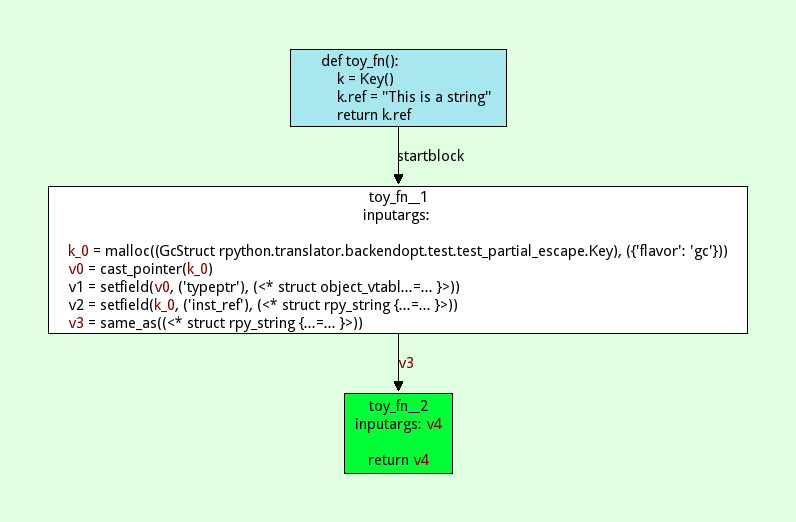
\includegraphics[width=0.8\textwidth]{simplest-func.png}
\caption{simplest diagram}
\label{figure-4}
\end{figure}

Σε αυτού του είδους τα γραφήματα δημιουργείται μόνο ένα \textit{state}. Το
\textit{state} είναι η δομή δεδομένων την οποία χρησιμοποιούμε για να
αποθηκεύουμε την κατάσταση των μεταβλητών (όπως λέει και το όνομα) σε κάθε
\texttt{Block}. Περιέχει δηλαδή τα εικονικά αντικείμενα που αναπαριστούν
μεταβλητές. Εάν μια μεταβλητή αναπαριστάται στο \textit{state} αυτό σημαίνει ότι
μέχρι τώρα δεν διαφεύγει και έχει αφαιρεθεί από τον κώδικα. Ένα το σύστημα
αντιληφθεί ότι διαφεύγει τότε την επανατοποθετεί στον κώδικα  (όπως αυτό
χρειάζεται βλ. malloc και casts) και την αφαιρεί από το \textit{state}.

Αφού βελτιστοποιήσουμε τις εντολές μέσα στο μοναδικό \texttt{Block}, συνεχίζουμε
με τις επιπλέον περιπτώσεις. Να σημειώσουμε ότι πιο πριν ξεκινήσαμε χωρίς να
πειράξουμε το \texttt{Block} καθόλου έτσι ώστε να δούμε αν το σύστημα αλλάζει
λόγω side-effects. Φυσικά δεν υπήρχαν.

\subsection{Split}

\begin{wrapfigure}{H}{6.5cm}
\caption{State split}
\label{wrapped-figure}
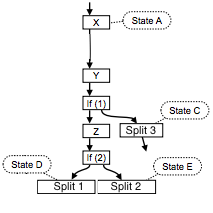
\includegraphics[width=6.5cm]{split-state.png}
\end{wrapfigure} 

Εδώ, στις συναρτήσεις (στις οποίες χρησιμοποιούνταν ως tests) είχαμε προσθέσει ένα
\textit{if}. Αυτό σημαίνει ότι η ροή θα μπορεί να ακολουθήσει δύο μονοπάτια
οπότε θα υπάρχουν παραπάνω από τρία \texttt{Block}s. Εμείς εδώ θα πρέπει να
προβλέψουμε το τι συμβαίνει σε όλα τα παρακλάδια της ροής εκτέλεσης.
Δημιουργούμε για αυτόν τον λόγο ένα \textit{state} για κάθε \texttt{Block}. Αν
έχουμε ένα \textit{split}, τότε το \textit{state} του αρχικού \texttt{Block} θα
αντιγραφεί στα άλλα \texttt{Block}s, και προφανώς το καθένα από αυτά θα
ακολουθήσει άλλη πορεία ζωής όταν γίνει η ανάλυση των επόμενων \texttt{Block}.
(Βλ. σχήμα \ref{wrapped-figure} δίπλα.)

Φυσικά αν υπάρχει \textit{split} από κάποιο \texttt{Block} με \textit{if}, τότε
θα υπάρχει και \textit{merge} σε κάποιο \texttt{Block} καθώς το
\textit{returnblock} κάθε γραφήματος είναι μοναδικό. Βέβαια όταν αυτό λαμβάνει
χώρα στο \textit{returnblock} δεν μας ενδιαφέρει καθώς το return γίνεται
αυτόματα και δεν πρέπει να αλλάξουμε κάτι, οπότε την διαχείριση των
\textit{merges} την έχουμε στο επόμενο επίπεδο δυσκολίας.

\subsection{Merge}

Σε αυτό το επίπεδο πολυπλοκότητας, δημιουργήσαμε tests και χειριστήκαμε τις
περιπτώσεις όπου τα \textit{merges} απαντώνται σε άλλα \texttt{Blocks} πλην
του \textit{returnblock}. Έπρεπε να διαχειριστούμε την ένωση δύο
\textit{state} μεταβλητών σε ένα. Εδώ ήταν το δυσκολότερο κομμάτι της
υλοποίησης καθώς οι λεπτομέρειες βρίθουν. Έπρεπε να ελέγξουμε και να
συγκρίνουμε τα δύο \textit{states}. Σε περίπτωση που ένα αντικείμενο υπήρχε
και στα δύο, τότε φυσικά έπρεπε να αντιγραφεί στο καινούργιο συγχωνευμένο και
να μεταφερθούν όλα τα περιεχόμενά του. Αυτή είναι η περίπτωση που το
αντικείμενο δεν έχει επηρεαστεί από το if branch (είτε δεν λάμβανε μέρος σε
αυτό) και μπορεί ακόμα να είναι εικονικό. Επίσης για να συμβεί το παραπάνω
πρέπει τα ορίσματα της εντολής δέσμευσης του αντικειμένου να είναι ίδια δηλαδή
το αντικείμενο να είναι πανομοιότυπο. Σε άλλες περιπτώσεις, δηλαδή όταν το
αντικείμενο είναι σε ένα από τα δύο \textit{states} dictionaries (είναι
εικονικό σε ένα μόνο branch), τότε το κάνουμε materialization και στα 2
branches, καθώς ο μεταγλωττιστής δεν μπορεί να ξέρει φυσικά σε ποιο θα
καταλήξει η ροή εκτέλεσης.

Σαφώς το \textit{merge} δεν λαμβάνει χώρα μόνο σε αυτές τις περιπτώσεις που
ξεκίνησαν με if αλλά και μετά από loops.

Να σημειώσουμε επίσης ότι η έκδοση της συνάρτησης που υλοποιεί το \textit{merge}
που παραθέτεται σε αυτή την εργασία είναι πολύπλοκη καθώς συμπεριλαμβάνει όλες
τις παραπάνω περιπτώσεις καθώς και τις περιπτώσεις των loops και του multi-merge
(βλ. επόμενη παράγραφος). Για μια πιο απλή κατανοητή έκδοση ανατρέχουμε στο log
του mercurial.

\subsection{Multi-merge}

Τα \textit{splits} είναι πάντα δυαδικά. Δηλαδή χωρίζονται σε δύο μόνο. Αν
υπάρχει τριπλό if case τότε το ένα από τα \texttt{Blocks} ξαναχωρίζεται. Τα
\textit{merges} όμως μπορούν να λάβουν χώρα όχι μόνο για δύο αλλά και για τρία
και παραπάνω \textit{Block}s σε ένα. Τότε η λογική για την συγχώνευση των
αντικειμένων \textit{state} θα πρέπει να τα λαμβάνει υπόψιν της.
Χρησιμοποιούμε ένα ζευγάρι για τον αρχικό έλεγχο – το οποίο είναι το αρχικό,
μοναδικό ζευγάρι στην περίπτωση απλής συγχώνευσης – και έπειτα εάν αυτός είναι
επιτυχής συγκρίνουμε με όσα αντικείμενα απομένουν. Η σύγκριση των ορισμάτων
για τον έλεγχο της ομοιότητας λαμβάνει χώρα στην – ορισμένη μέσα στο
αντικείμενο \texttt{VirtualObject} – μέθοδο \texttt{identical\_malloc\_args()}.

\subsection{Loops}

Η λογική των βρόγχων (loops) ήταν η δυσκολότερη. Μέχρι τώρα δεν έχουμε λάβει
υπόψιν μας τα loops στην λογική του προγράμματος. Όταν ο μεταγλωττιστής
εντοπίσει μια μεταβλητή που παίρνει μέρος σε ένα loop τότε την εξαναγκάζει να
διαφύγει. Ένα μεγάλο κομμάτι της σχεδίασης παρόλα αυτά (ακόμα και χωρίς την
κεντρική λογική) έχει υλοποιηθεί, και αυτό είναι το κομμάτι της διαχείρισης της
σειράς με την οποία \textit{βλέπουμε} και \textit{επεξεργαζόμαστε} τα
\texttt{Block}s (βλ. \textbf{worklist}). Στα μελλοντικά μας σχέδια
περιλαμβάνεται η πλήρης υλοποίηση της λογικής των loops. Παράδειγμα του πως
φαίνεται και υλοποιείται ένα γράφημα με loops δίνεται στο σχήμα \ref{figure-5}.

\begin{figure}[h]
\centering
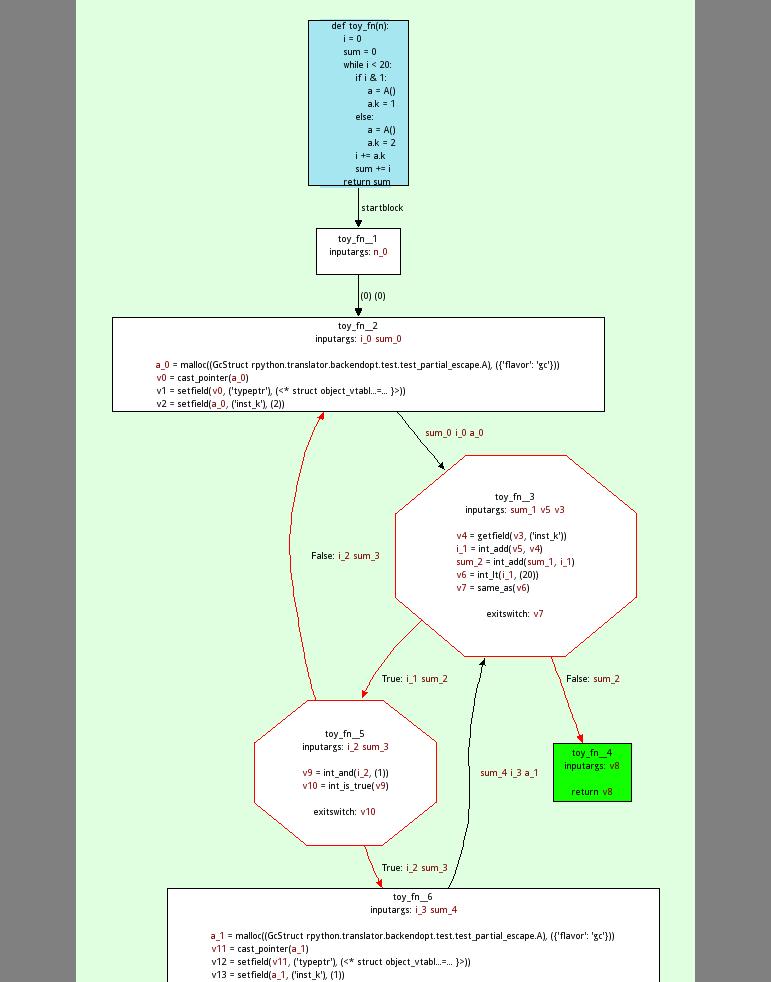
\includegraphics[width=0.7\textwidth]{loop-func.png}
\caption{loop diagram}
\label{figure-5}
\end{figure}

\subsection{Function Calling etc}

Τέλος υπάρχουν επιπλέον επίπεδα πολυπλοκότητας που το σύστημα μπορεί να τα
διαχειριστεί μόνο του ή πολύ απλά η διαχείρισή τους να είναι τετριμμένη. Λ.χ. η
κλήση άλλων συναρτήσεων με την εντολή \texttt{direct\_call()} μπορεί απλά να
μείνει αυτούσια και να μην επηρεάζει την λογική μας. Φυσικά λαμβάνουμε υπόψιν τα
ορίσματα που παίρνει και επιστρέφει, καθώς αυτά μπορούν προφανώς να την
επηρεάσουν λ.χ. με την χρήση ενός αντικειμένου ως όρισμα.

%------------------------------------------------------------------------------

\section{Γενικά για προβλήματα}

Αρχικά να σημειώσουμε ότι δεν αντιμετωπίσαμε πολλά από τα προβλήματα που
αναφέρονταν στο paper\cite{stadler2014partial} που βασιζόμαστε, με βασικότερο
όλων την έλλειψη μηχανισμών κλειδώματος (locking). Αυτό το αποφύγαμε λόγω του
καθολικού κλειδώματος που υπάρχει στην Python και στην πλειοψηφία των
υλοποιήσεών της (Global Interpreter Lock – GIL). Το πρόβλημα με αυτή την
περίπτωση έγκειτο στο να συνειδητοποιήσουμε ότι δεν απαιτούνται επιπλέον
ενέργειες για την κάλυψη του locking.\cite{gil} Τα περισσότερα προβλήματα που
αντιμετωπίσαμε είχαν να κάνουν κυριώς με περιπτώσεις τις οποίες δεν είχαμε
σκεφτεί και δεν είχαμε προβλέψει.

\subsection{Edge cases}

Όπως είπαμε, σε ένα τέτοιο εγχείρημα, ακόμα και με την καλύτερη ανάλυση και τον
καλύτερο σχεδιασμό, θα προκύψουν θέματα που ο προγραμματιστής δεν είχε σκεφτεί.
Αυτά είναι τα λεγόμενα \textit{edge cases} του σχεδιασμού της λογικής του
προγράμματος. Στην προσπάθειά μας για την υλοποίηση του module βρεθήκαμε μπροστά
σε πολλές τέτοιες περιπτώσεις. Το μεγαλύτερο παράδειγμα είναι η παρακάτω
περίπτωση.

\subsubsection{Περίπτωση Αναγκαιότητας Extra Block}

Η περίπτωση αυτή ήταν ίσως η δυσκολότερη στην ανακάλυψή της καθώς δεν οδηγούσε
σε \textit{complilation error} ούτε σε \textit{segmentation fault} αλλά μόνο σε
μη αποδοτικό κώδικα σε κάποιες πολύ συγκερκιμένες καταστάσεις. Θα εξηγήσουμε το
παράδειγμα αυτό και με εικόνες που δείχνουν το πρόβλημα καθώς είναι δύσκολο στην
κατανόησή του. Το πρόβλημα αυτό λάμβανε χώρα διότι σε κάποιες περιπτώσεις με
branch στην ροή του προγράμματος στις οποίες κανονικά τα αντικείμενα θα έπρεπε
να παραμείνουν εικονικά στην μια, αυτά επανατοποθετούνταν στον κώδικα και για τα
δύο branches της ροής. Αυτό όπως ανακαλύψαμε έχει να κάνει με την ανικανότητα
του μεταγλωττιστή να βρει ένα σωστό σημείο για να επανατοποθετήσει τις εντολές
δέσμευσης και αρχικοποίησης του αντικειμένου.

Στο \ref{figure-8:a} φαίνεται ένα διάγραμμα που έχει ακριβώς αυτό το πρόβλημα.
Το σημείο που έβρισκε ήταν το \texttt{Block} που ήταν ο μόνος κοινός "πρόγονος"
του branch, οπότε οι εντολές τοποθετούνταν εκεί, άρα ουσιαστικά το αντικείμενο
δεν ήταν εικονικό πλέον σε κανένα από τα branches. Ανάμεσα στο \textit{if}
\texttt{Block} και στο αριστερό παιδί του απαιτείται ένα επιπλέον \texttt{Block}
για αυτές τις εντολές διότι το αντικείμενο εκεί θα πρέπει να \textit{υπάρχει}
καθώς εκεί καταλήγει και ένα \texttt{Link} με μια σταθερά (βλ. το αριστερότερο
κόκκινο βελάκι στο \ref{figure-8:a}). Από την άλλη όμως, στο δεξιό παιδί το
αντικείμενο δεν χρειάζεται να υπάρχει και μπορεί να παραμείνει εικονικό.

\begin{figure}[h]
\begin{subfigure}{0.6\textwidth}
\centering
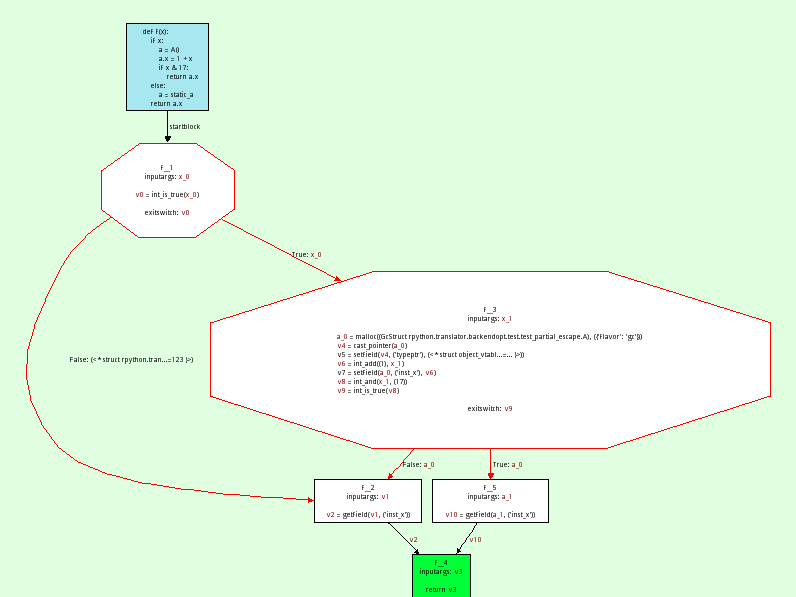
\includegraphics[width=\textwidth]{needs-extra-block-bef.png}
\caption{Extra Block Problem}
\label{figure-8:a}
\end{subfigure}
\begin{subfigure}{0.4\textwidth}
\centering
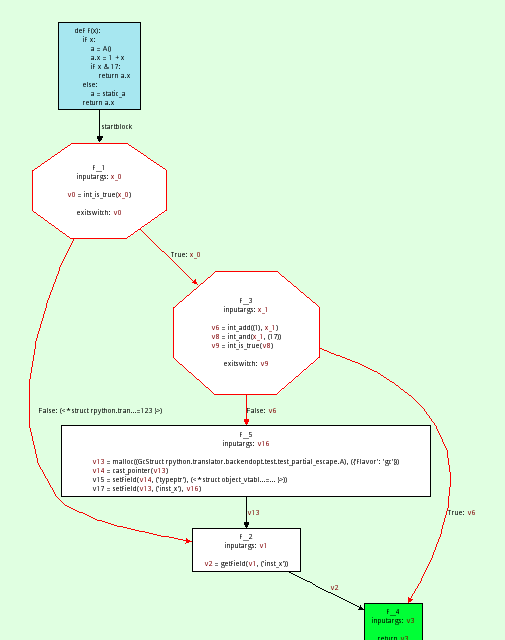
\includegraphics[width=1.05\textwidth]{needs-extra-block-after.png}
\caption{Extra Block Problem Solution}
\label{figure-8:b}
\end{subfigure}
\end{figure}

Στο \ref{figure-8:b} φαίνεται το διάγραμμα μετά την λύση που εφαρμόσαμε. Το
επιπλέον \texttt{Block} έχει τώρα τον κώδικα δέσμευσης, οπότε αυτό οδηγεί στο
\textit{materialization} του αντικειμένου \textit{μόνο} στο branch που θέλουμε.

Όπως είπαμε η λύση αυτού του θέματος ήταν πολύπλοκη. Η ανεύρεση των περιπτώσεων
που απαιτούνται τα επιπλέον \texttt{Block}s πριν την έναρξη του editing του κάθε
\texttt{Block} ήταν εξαιρετικά πολύπλοκη. Από την άλλη εάν αποφασίζαμε να
αποφανθούμε την ανάγκη των επιπλέον \texttt{Blocks}s κατά το editing, τότε
υπήρχε τεράστιο πρόβλημα στην εισαγωγή του \texttt{Block} καθώς αυτό οδηγούσε
στην ανάγκη επιπλέον ενεργειών για την επεξεργασία των (ήδη-επεξεργασμένων)
\texttt{Link}s και \textit{arguments}. Οπότε αποφασίσαμε στην τοποθέτηση ενός
άδειου \texttt{Block} σε κάθε \texttt{Link} του διαγράμματος! Αυτό φαίνεται στο
διάγραμμα \ref {figure-8c}. Μπορεί με την πρώτη ματιά αυτό να ακούγεται
υπερβολικό και καθόλου αποδοτικό, όμως δεν είναι. Όταν η ειδική
συνάρτηση\footnote{\texttt{(insert\_links())}} – η οποία ανατρέχει το πρόγραμμα
πρώτη πριν την έναρξη της ανάλυσης – ανακαλύψει ένα \texttt{Link} τότε τοποθετεί
ένα άδειο \texttt{Block} στο κέντρο και μεταβάλει αναλόγως τα \textit{in \& out}
\texttt{Link}s του, έτσι ώστε να "τρέχει" φυσικά στο ενδιάμεσο. Έπειτα η ανάλυση
ξεκινά – τα περισσότερα από αυτά τα καινούργια \texttt{Block}s θα παραμείνουν
άδεια, και στο τέλος θα τρέξει η συνάρτηση \textit{καθαρισμού}
\texttt{eliminate\_empty\_blocks())}, η οποία θα κάνει αυτό ακριβώς που αναφέρει
το όνομά της – θα αφαιρέσει τα άδεια \texttt{Block}s. Επίσης τρέχουμε την
συνάρτηση \texttt{join\_blocks())} η οποία συγχωνεύει τυχών συνεχόμενα
\texttt{Block}s που δεν έχουν λόγο να είναι χωρισμένα (π.χ. \textit{if case}).

\begin{figure}[h]
\centering
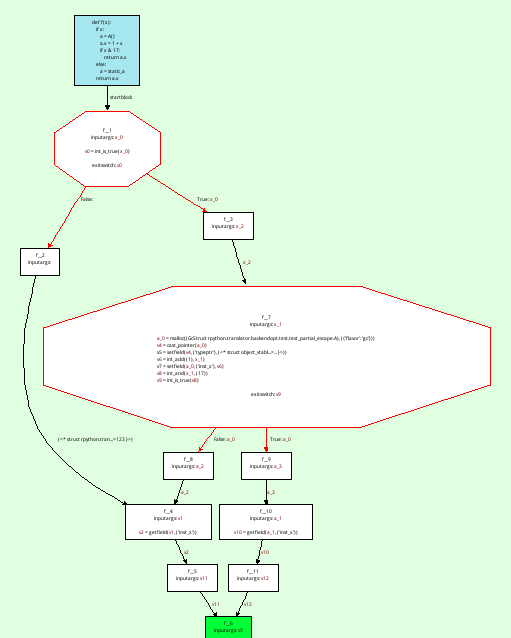
\includegraphics[width=0.8\textwidth]{needs-extra-block-med.png}
\caption{Extra Block Problem Solution (before cleaning up)}
\label{figure-8c}
\end{figure}


%------------------------------------------------------------------------------
%------------------------------------------------------------------------------

\chapter{Αποτελέσματα – Συμπεράσματα}
\label{chapter5}

\section{Γενικά}

Σε αυτό το τελευταίο κεφάλαιο θα δώσουμε τα τελικό αποτελέσματα του εγχειρήματος
και μερικές παρατηρήσεις για τον κώδικα αυτόν. Θα προσπαθήσουμε να δώσουμε στον
αναγνώστη το μέγεθος της βελτίωσης που καταφέραμε να πετύχουμε με αυτόν τον
βελτιστοποιητή. Αξίζει να επαναλάβουμε εδώ ότι ο βελτιστοποιητής μας τρέχει κατά
το compile time του μεταγλωττιστή pypy και εφαρμόζεται πάνω στον κώδικά του ανά
συνάρτηση. Στοχεύουμε φυσικά στο να βελτιώσουμε τον χρόνο (και γενικότερα το
``κόστος") των συναρτήσεων αυτών. Στις μετρήσεις που ακολουθούν επικεντρωνόμαστε
στο χρονικό κόστος.

Να υπογραμμίσουμε εδώ ότι οι μετρήσεις έγιναν μόνο σε ένα machine (με Mac OS X
10.11.4 σε επεξεργαστή 2.3GHz Intel Core i5, 16GB 1333MHz RAM και SSD δίσκο) και
δεν προσπαθήσαμε να βρούμε κάποιο πιθανοτικό μοντέλο ή κατανομή, στην οποία θα
μπορούσαμε να εντάξουμε το data set των συναρτήσεών μας. Τα περισσότερα νούμερα
που παραθέτουμε, όπως θα δούμε, είναι μέσοι όροι, και πολλές φορές μέσοι όροι
από μέσους όρους για λόγους που θα δούμε παρακάτω. Πειραματιστήκαμε με πολλούς
μεθόδους για το πως θα μετρήσουμε την βελτιστοποίηση. Η αρχική σκέψη ήταν η απλή
σύγκριση τιμών χρόνου αλλά οι συναρτήσεις στις οποίες εφαρμόζεται η
βελτιστοποίηση μας είναι περισσότερες από 100000.

\section{Μετρήσεις}

\subsection{Getfield Removal}

Η πρώτη μετρική είναι μια απλή καταμέτρηση των εμφανίσεων της πιο συχνής και
ακριβής εντολής\footnote{Η εντολή \texttt{getfield} δεν είναι στην
πραγματικότητα η πιο ακριβή ως μονάδα, αλλά σίγουρα η πιο συχνή οπότε η πιο
ακριβή ως σύνολο.}, της \texttt{getfield}, που απλά στοχεύουμε να μειώσουμε.
Στην έκδοση του κώδικά μας που παραθέτουμε στο παράρτημα, η καταμέτρηση αυτή
γίνεται σε κάθε iteration μέσα στην κεντρική συνάρτηση και ο αριθμός
επιστρέφεται για ευκολότερη χρήση, και γρήγορα νούμερα. Φυσικά, κατά την
διαδικασία μέτρησης, γράψαμε διάφορα scripts για καλύτερα νούμερα. Αυτά τα
κομμάτια κώδικα θα αφαιρεθούν στην τελική έκδοση.

Η βελτιστοποίησή μας τρέχει πολλές φορές – αν και πάντα τελευταία όπως είπαμε –
κατά το στάδιο των βελτιστοποιήσεων αλλά τα δύο πρώτα runs είναι τα πιο
σημαντικά. Σε αυτά σκανάρονται οι πιο σημαντικές και βασικές συναρτήσεις του
framework. Παρακάτω στον πίνακα \ref{table-getfield} φαίνεται τα μέσα ποσοστά
των αριθμών των \texttt{getfield} εντολών που καταφέραμε να αφαιρέσουμε και ο
αριθμός όσων γραφημάτων αλλάξαμε. Τα ποσοστά δηλαδή περιλαμβάνουν μόνο τα
γραφήματα που άλλαξαν. Όπως μπορούμε να δούμε ένα περίπου 90\% των γραφημάτων
δεν άλλαξαν καθόλου. Αυτό μπορεί να οφείλεται σε πολλούς λόγους, είτε απλότητας
των γραφημάτων (οπότε και η βελτιστοποίηση γίνεται σε προηγούμενα στάδια) είτε
ανικανότητα της μεθόδου μας να ``πιάσουμε" τις πιθανές προς αφαίρεση μεταβλητές
λόγω μεγάλης πολυπλοκότητας του γραφήματος.

\begin{table}[]
\centering
\caption{General median percentage of getfield removal after partial escape application}
\label{table-getfield}
\begin{tabular}{lllll}
–– & \cellcolor[HTML]{C0C0C0}Total graphs/functions &
\cellcolor[HTML]{C0C0C0}Graphs that changed & \cellcolor[HTML]{C0C0C0}Getfield removal &  \\
\cellcolor[HTML]{C0C0C0}1o run & \multicolumn{1}{c}{21320} & \multicolumn{1}{c}{2154} & \multicolumn{1}{c}{18\%} &  \\
\cellcolor[HTML]{C0C0C0}2o run & \multicolumn{1}{c}{59433} & \multicolumn{1}{c}{3281} & \multicolumn{1}{c}{7\%} &  \\
 &  &  &  & 
\end{tabular}
\end{table}

Μπορούμε να βγάλουμε ένα γενικό συμπέρασμα ότι αφαιρούμε περίπου το 5\% των
εντολών από όλο το codebase του PyPy – είτε οποιουδήποτε Python codebase δοθεί.

\subsection{Malloc Removal}

Στη συνέχεια αποφασίσαμε να συλλέξουμε μετρήσεις για την ``ισχυρή" και ``ακριβή"
\texttt{malloc}. Εδώ η διαδικασία μετρήσεων είναι πιο πολύπλοκη καθώς η
βελτιστοποίηση αυτή τείνει να μην αφαιρεί τις εντολές αυτές με την ``συμβατική"
έννοια (δηλαδή να μειώνει τα \textit{counts} στον κώδικα) αλλά να μειώνει την
χρήση τους και πιο συγκεκριμένα την χρήση μνήμης εξωτερικής του \textit{stack}.

Επιπλέον υπάρχει ακόμα και η περίπτωση αύξησης του αριθμού των \texttt{malloc}
καθώς πολλές φορές έχουμε το εξής φαινόμενο: Αρχικά το αντικείμενο κρίνεται μη
απαραίτητο σε αυτό το σημείο του scan και αφαιρείται. Έπειτα, σε μερικά branches
της ροής εκτέλεσης μπορεί να κριθεί ότι απαιτείται και να επανατοποθετηθεί. Αυτό
μπορεί να γίνει σε μερικά branches λόγω του partiality της μεθόδου. Αφού τα
γραφήματα περνούν ήδη πιο πριν από συμβατικό escape analysis, αυτό το use case
θα είναι το πιο συχνό στο οποίο η δικιά μας βελτιστοποίηση θα δουλέψει. Για αυτό
το λόγω απλά θα μετρήσουμε εδώ τα γραφήματα, τα οποία επηρεάστηκαν (βλ. \ref
{table-malloc}).

\begin{table}[h]
\centering
\caption{Malloc changes}
\label{table-malloc}
\begin{tabular}{lllll}
–– & \cellcolor[HTML]{C0C0C0}Total graphs & \cellcolor[HTML]{C0C0C0}Mallocs got removed in... & \cellcolor[HTML]{C0C0C0} Mallocs got moved in... &  \\
\cellcolor[HTML]{C0C0C0}1o run & \multicolumn{1}{c}{21243} & \multicolumn{1}{c}{8} & \multicolumn{1}{c}{231} &  \\
\cellcolor[HTML]{C0C0C0}2o run & \multicolumn{1}{c}{59066} & \multicolumn{1}{c}{22} & \multicolumn{1}{c}{366} &  \\
 &  &  &  & 
\end{tabular}
\end{table}


Για να δείξουμε ότι παρόλα αυτά ο χρόνος φυσικά μειώνεται έχουμε την επόμενη
μετρική, η οποία Θα μετρήσει το μέσο κόστος της κάθε συνάρτησης.

\subsection{Time Cost}

Τέλος, θα δώσουμε μέσα κόστη εκτέλεσης. Καταλήξαμε στους μέσους όρους κόστους
εκτέλεσης (\textit{median executin cost}) καθώς φυσικά μιλάμε για υπολογιστικά
συστήματα οπότε το ένα run από το άλλο, ακόμα και της ίδιας συνάρτησης, μπορεί
να διαφέρει εκπληκτικά χρονικά. Χρησιμοποιούμε την συνάρτηση \\
\texttt{measure\_median\_execution\_cost()} του module \texttt{inline} στο PyPy
η οποία είναι εξαιρετικά βοηθητική και αποτέλεσε βασικό κομμάτι των μετρήσεών
μας. Η συνάρτηση αυτή, δοθείσας μιας συνάρτησης, επιστρέφει πάντα το ίδιο
νούμερο· το μέσο κόστος εκτέλεσης, οπότε ξέρουμε ότι είναι μια καλή μετρική.
Παρακάτω, στον πίνακα \ref{table-time} παραθέτουμε τα χρονικά κέρδη που είχαμε
σε ποσοστά. Τα ποσοστά βγήκαν φυσικά μεταξύ δύο runs της παραπάνω συνάρτησης
μέτρησης. Τρέχουμε πρώτα το αρχικό γράφημα που παίρνουμε από τον μεταγλωττιστή,
και αφού πάρουμε ένα μέσο κόστος για αυτό, περνάμε το γράφημα από τον
βελτιστοποιητή μας. Τέλος παίρνουμε άλλο ένα μέσο κόστος και βγάζουμε το
ποσοστό. Από όλα αυτά τα ποσοστά – για τα γραφήματα που επηρεάστηκαν – βγάζουμε
ένα γενικό ποσοστό. Αυτά δίνονται παρακάτω.

\begin{table}[h]
\centering
\caption{Time gains throughout all graphs}
\label{table-time}
\begin{tabular}{lllll}
–– & \cellcolor[HTML]{C0C0C0}Total graphs/functions & \cellcolor[HTML]{C0C0C0}Graphs that changed & \cellcolor[HTML]{C0C0C0}Time gain &  \\
\cellcolor[HTML]{C0C0C0}1o run & \multicolumn{1}{c}{21320} & \multicolumn{1}{c}{2230} & \multicolumn{1}{c}{4.5\%} &  \\
\cellcolor[HTML]{C0C0C0}2o run & \multicolumn{1}{c}{59433} & \multicolumn{1}{c}{4157} & \multicolumn{1}{c}{5.2\%} &  \\
 &  &  &  & 
\end{tabular}
\end{table}
Μπορούμε να βγάλουμε ένα γενικό συμπέρασμα ότι βελτιώνουμε περίπου κατά 1\% την
ταχύτητα του PyPy!

Όπως βλέπουμε και εδώ, δεν αλλάζουν όλα τα γραφήματα, αλλά σιγουρευτήκαμε, κατά
το tesing phase με πολλούς τρόπους, ότι ο χρόνος δεν αυξάνεται
(\textit{overhead}) σε απολύτως κανένα γράφημα. Βλέπουμε επίσης ότι οι αριθμοί
των γραφημάτων που άλλαξαν είναι περίπου ίδιοι και αυτό είναι λογικό αφού στα
γραφήματα που μπορέσαμε και αφαιρέσαμε εντολές, ο χρόνος αναμένουμε να είναι
σαφώς γρηγορότερος, όπως και είναι.


Να τονίσουμε εδώ ξανά ότι η βελτιστοποίηση αυτή τρέχει τελευταία· μετά από όλες
τις υπόλοιπες που υπάρχουν μέσα στο ώριμο PyPy project και μετά και από το
normal partial escape analysis που υπάρχει. Σε αντίθετη περίπτωση είμαστε
σίγουροι ότι ο βελτιστοποιητής θα ήταν πολύ πιο παραγωγικός.

Σημείωση: Τα πλήρη logs των μετρήσεων βρίσκονται εδώ:
\href{}{github.com/papanikge/thesis}

%------------------------------------------------------------------------------

\section{Μελλοντική εργασία}

Το παρόν εγχείρημα προέκυψε παραγωγικό και σύμφωνα με τα νούμερα που παραγάγαμε
πολύ αποτελεσματικό! Πραγματοποιήσαμε και προσφέραμε στο ευρύ κοινό μια
υλοποίηση της μεθόδου ανάλυσης μερικής διαφυγής και βελτιστοποίησης μέσω
αντικατάστασης βαθμωτών και συμβάλαμε φυσικά με τον δική μας μικρή βοήθεια στην
βελτίωση της ταχύτητας του μεταγλωττιστή του PyPy.

Ο μεγάλος όγκος των \texttt{malloc}s αφαιρούνται κατά την πρώτη \textit{build-
in} βελτιστοποίηση του PyPy (\textit{non-partial escape
analysis}\footnote{escape.py}). Η δικιά μας μέθοδος πυροδοτείται αργότερα και
παρόλα αυτά επιτυγχάνει να αποφύγει περισσότερα \texttt{getfield}s.

Καταλήξαμε ότι δεν μπορεί να γίνει ανάλυση και υλοποίηση της μεθόδου αυτής για
δυναμικές γλώσσες χωρίς να λάβουμε υπόψιν μας το aliasing και τις λεπτομέρειες
που επιφέρει. Φυσικά αυτό το πρόβλημα δεν υπάρχει στις στατικές γλώσσες καθώς ο
προγραμματιστής φροντίζει για τους τύπους, ενώ στην περίπτωση μας είναι
αρμοδιότητα του μεταγλωττιστής μας, οπότε το aliasing των τύπων υπεισέρχεται
σχεδόν σε όλη την έκταση των προγραμμάτων.

Μελλοντικές εργασίες περιλαμβάνουν πλήρης υλοποίηση της λογικής των loops
καθώς τώρα η υλοποίησή μας τα αγνοεί κάνοντάς τα όλα να διαφύγουν.
%------------------------------------------------------------------------------

\chapter{Συμπεράσματα - Μελλοντική Εργασία}
\label{chapter6} 

Το παρόν εγχείρημα προέκυψε παραγωγικό. Πραγματοποιήσαμε και προσφέραμε στο ευρή
κοινό μια υλοποίηση της μεθόδου ανάλυσης μερικής διαφυγής και βελτιστοποίησης
μέσω αντικατάστασης βαθμωτών και συμβάλαμε φυσικά με τον δική μας μικρή βοήθεια
στην βελτίωση της ταχύτητας του μεταγλωττιστή του PyPy.

Βλέπουμε από το προηγούμενο κεφάλαιο τα νούμερα. (todo)

Ο μεγάλος όγκος των \texttt{malloc}s αφαιρούνται κατά την πρώτη \textit{build-
in} βελτιστοποίηση του PyPy (\textit{non-partial escape
analysis}\footnote{escape.py}). Η δικιά μας μέθοδος πυροδοτείται αργότερα και
παρόλα αυτά επιτυγχάνει να αποφείγει περισσότερα \texttt{getfield}s.

Καταλήξαμε ότι δεν μπορεί να γίνει ανάλυση και υλοποίηση της μεθόδου αυτής για
δυναμικές γλώσσες χωρίς να λάβουμε υπόψιν μας το aliasing και τις λεπτομέρεις
που επιφέρει. Φυσικά αυτό το πρόβλημα δεν υπάρχει στις στατικές γλώσσες καθώς ο
προγραμματιστής φροντίζει για τους τύπους, ενώ στην περίπτωση μας είναι
αρμοδιότητα του μεταγλωττιστής μας, οπότε το aliasing των τύπων υπεισερχεται
σχεδόν σε όλη την έκταση των προγραμμάτων.

%------------------------------------------------------------------------------

%-----------------------------------------------------------

\appendix 
\chapter{Κώδικας - Code listing}
\lstinputlisting[language=Python]{partial_escape.py}

%-----------------------------------------------------------
% BIBLIOGRAPHY
\printbibliography
%%%%%%%%%%%%%%%%%%%%%%%%%%%%%%%%%%%%%%%%%%%%%%%%%%%%%%%%%%%%
%	THE END
%%%%%%%%%%%%%%%%%%%%%%%%%%%%%%%%%%%%%%%%%%%%%%%%%%%%%%%%%%%%

\end{document}  